% ========================================= TEMPLATE INFO ========================================
%
% Author:       P4ntomime
% Version:      1.0.0
% Last updated: 2024-02-18
% Brief:        A LaTeX template for summaries. See README.md for more information.
% 
% ================================================================================================
\documentclass[8pt, a4paper, twoside]{extarticle}
% Font size:    8pt
% Paper size:   A4
% style:        twoside (needed, so odd and even pages have different margins)
% orientation:  portrait. (use 'landscape' for landscape orientation)


% ========================================= DOCUMENT INFO =========================================
\def\title{Elektronik 1}           						% title
\def\shorttitle{Elo1} 									% short title (displayed as PDF title)
\def\dozent{Prof. Guido Keel}         					% lecturer
\def\semester{HS 2023}     								% semester
\def\author{Simone Stitz}        						% author(s)
\def\repo{https://gitlab.com/sstitz/elektronik-1}       % repository link
\def\version{2.0.\today}    							% version
\def\pagelimit{10}          			 				% page limit -> causes pages after limit to be red
\def\titleoption{compact}   							% options: compact, normal
\def\enableToC{false}

% ================================= PACKAGES, SETUP AND COMMANDS ==================================
\input{preamble.tex}

% =========================================== DOCUMENT ============================================
\begin{document}
    \begin{layout}
        \section{Quellen}

\begin{tabular}{ll}
    Thévenin    & Spannungsquelle mit Seriewiderstand \\
    Norton      & Stromquelle mit Parallelwiderstand
\end{tabular}

\vspace{0.1cm}

\crd{\textbf{ \textrightarrow\ DC- und AC-Signale werden separat betrachtet!} }


\subsection{Superpositionsprinzip}

Eingangssignale eines \textbf{linearen Netzwerks} dürfen separat betrachtet werden. \\
(nur eine Quelle aktiv, die anderen Quellen werden ausgeschaltet)

\vspace{0.1cm}

\textbf{ \textrightarrow\ Superpositionsprinzip funktioniert nicht in der Sättigung!}


\section{Grundlagen}

\subsection{Kleinsignal-Ersatzschaltung (!)}
\label{kleinsignal-ersatzschlatung}

\textbf{Ziel:} Berechnung der \textbf{AC-Spannungen} an den verschiedenen Knoten der Schaltung sowie der Wechselströme in allen 
Zweigen der Schaltung.

\vspace{0.1cm}

\begin{itemize}
    \item DC-Spannungsquellen durch Kurzschlüsse ersetzen
    \item DC-Stromquellen entfernen (Unterbrüche)
    \item Nichtlineare Bauteile mit Kleinsignal-Ersatzschlatung ersetzen
    \item Koppel- und Bypass-Kondensatoren kurzschliessen
    \item Spulen entfernen
\end{itemize}


\subsection{Schaltungsanalyse - Vorgehen (!)}

\textbf{DC-Arbeitspunkte und Verstärkungsfaktor bestimmen}

\vspace{0.1cm}

\begin{itemize}
    \item Arbeitspunkte bestimmen (DC-Spannung in jedem Knoten)
    \item Kleinsignalersatzschaltung gemäss Kapitel \ref{kleinsignal-ersatzschlatung} bilden
    \item Schaltung ggf. umzeichnen und vereinfachen
    \item Verstärkung $\frac{V_{\rm out}}{V_{\rm in}}$ berechnen 
\end{itemize}


\subsection{Dezibel}

\vspace{-0.2cm}

\begin{center}
    \renewcommand{\arraystretch}{2}
    \begin{tabular}{c c c}
        \myul{\textbf{Dezibel}}                                                                                             &               & \myul{\textbf{Faktor}}                                \\
        $A_{\deci \bel}  = 20 \log \Biggl( \Bigl|\underbrace{\frac{V_{\rm out}}{V_{\rm in}}}_{\substack{A}} \Bigr| \Biggr)$ & \textlrarrow\ & $A  = 10^{\frac{A_{\deci \bel}}{20 \, \deci \bel}}$   \\
        $A_{\rm total} = A_{\deci \bel 1} + A_{\deci \bel 2}$                                                               &               & $A_{\rm total} = A_1 \cdot A_2$                       
    \end{tabular}
    \renewcommand{\arraystretch}{1}
\end{center}


\section{Verstärker}

\subsection[Übertragungsfaktor (reale Verstärker)]{Übertragungsfaktor $\bm{k}$ (reale Verstärker)}

\begin{center}
    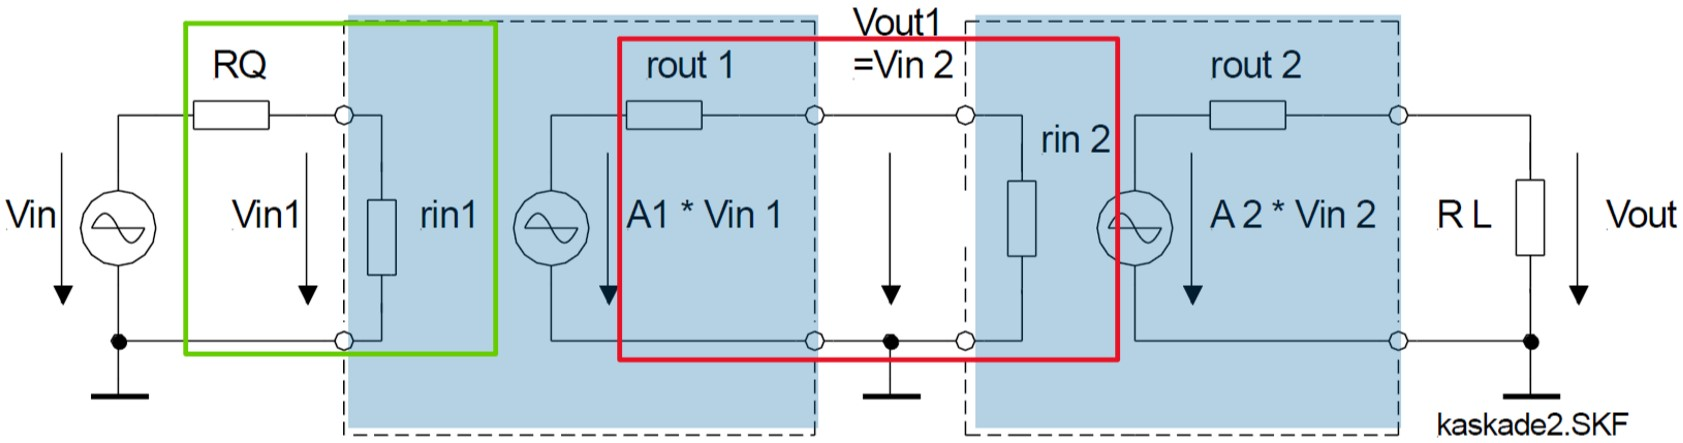
\includegraphics[width=0.75\columnwidth]{images/kopplungsfaktor.jpg}
\end{center}

\begin{tabular}{lll}
    $ V_{\rm in1} = V_{\rm in} \cdot \cgn{ \underbrace{ \frac{R_{\rm in1}}{R_{\rm in1} + R_Q} }_{\substack{k_1}} } $            &
    $ V_{\rm in2} = \crd{\underbrace{ \frac{R_{\rm in2}}{R_{\rm in2} + R_{\rm out1}} }_{\substack{k_2}} } \cdot V_{\rm out1} $  &
    $ V_{\rm out} = V_{\rm in} \cdot k_1 \cdot A_1 \cdot k_2 \cdot A_2 \cdot k_L $
\end{tabular}


		\section{Operationsverstaerker}

\subsection{Eigenschaften eines OpAmps}

\begin{minipage}{0.6\columnwidth}
	\begin{center}
		% LTeX: enabled=false
\resizebox{0.6\columnwidth}{!}{
    \begin{circuitikz}
        \tikzstyle{every node}=[font=\Huge]
        \draw [line width=1pt, short] (0,0) -- (7.75,4.5);
        \draw [line width=1pt, short] (0,0) -- (0,9);
        \draw (4.25,4.5) to[american voltage source] (2.75,3);
        \draw [line width=1pt, short] (7.75,4.5) -- (0,9);
        \node at (1,2.5) {\textbf{+}};
        \node at (1,6.5) {\textbf{-}};
        \draw (0.5,2.5) to[european resistor] (0.5,6.5);
        \draw (0.5,2.5) to[short, -o] (-1.75,2.5) ;
        \draw (0.5,6.5) to[short, -o] (-1.75,6.5) ;
        \draw [<->, >=Stealth] (-0.5,2.5) -- (-0.5,6.5)node[pos=0.5, fill=white]{$V_{in}$};
        \node at (1.75,4.5) {$Z_i = \infty$};
        \draw (2.75,3) to (2.75,2.75) node[ground]{};
        \node at (4.5,3.25) {$a = \infty$};
        \draw (4.25,4.5) to[european resistor] (6,4.5);
        \draw (6,4.5) to[short, -o] (9,4.5) ;
        \draw [->, >=Stealth] (-2,2) -- (-0.25,2)node[pos=0.5, fill=white]{$I_{in}=0$};
        \node at (8.5,5) {$V_{out}$};
        \draw [->, >=Stealth] (-1.75,7) -- (-0.25,7)node[pos=0.5, fill=white]{$I_{in}=0$};
        \node at (5,5) {$Z_{out} = 0$};
    \end{circuitikz}
}%
%Tikzmaker code:
%[[],[{"x":0,"y":850},{"x":387.5,"y":625},"Line",1,"\\draw [line width=1pt, short] (0,0) -- (7.75,4.5);","",[0,0,0],[255,255,255],0,false,[0,0,0,0],1,{"fontSize":32,"textPlacement":0.5,"isBold":false,"isItalic":false,"hasUnderline":false,"alignmentText":"center"}],[{"x":0,"y":850},{"x":0,"y":400},"Line",3,"\\draw [line width=1pt, short] (0,0) -- (0,9);","",[0,0,0],[255,255,255],0,false,[0,0,0,0],1,{"fontSize":32,"textPlacement":0.5,"isBold":false,"isItalic":false,"hasUnderline":false,"alignmentText":"center"}],[{"x":212.5,"y":625},{"x":137.5,"y":700},"Voltage Source (American)",5,"\\draw (4.25,4.5) to[american voltage source] (2.75,3);","",[0,0,0],[255,255,255],0,false,32,0.4,{"isBold":false,"isItalic":false,"hasUnderline":false,"rotation":0,"frequency":1,"amplitude":1,"phase":0,"multiwire":0,"alignmentText":"center","endNodeType":"circ"}],[{"x":387.5,"y":625},{"x":0,"y":400},"Line",7,"\\draw [line width=1pt, short] (7.75,4.5) -- (0,9);","",[0,0,0],[255,255,255],0,false,[0,0,0,0],1,{"fontSize":32,"textPlacement":0.5,"isBold":false,"isItalic":false,"hasUnderline":false,"alignmentText":"center"}],[{"x":50,"y":725},{"x":50,"y":725},"Text",8,"\\node [font=\\LARGE] at (1,2.5) {\\textbf{+}};","+",[0,0,0],[255,255,255],0,false,32,0.4,{"isBold":true,"isItalic":false,"hasUnderline":false,"rotation":0,"frequency":1,"amplitude":1,"phase":0,"multiwire":0,"alignmentText":"center","endNodeType":"circ","isMathMode":false}],[{"x":50,"y":525},{"x":50,"y":525},"Text",9,"\\node [font=\\LARGE] at (1,6.5) {\\textbf{-}};","-",[0,0,0],[255,255,255],0,false,32,0.4,{"isBold":true,"isItalic":false,"hasUnderline":false,"rotation":0,"frequency":1,"amplitude":1,"phase":0,"multiwire":0,"alignmentText":"center","endNodeType":"circ","isMathMode":false}],[{"x":25,"y":725},{"x":25,"y":525},"Resistor (IEC)",10,"\\draw (0.5,2.5) to[european resistor] (0.5,6.5);","",[0,0,0],[255,255,255],0,false,32,0.4,{"isBold":false,"isItalic":false,"hasUnderline":false,"rotation":0,"frequency":1,"amplitude":1,"phase":0,"multiwire":0,"alignmentText":"center","endNodeType":"circ","isMathMode":true}],[{"x":25,"y":725},{"x":-87.5,"y":725},"End node",12,"\\draw [](0.5,2.5) to[short, -o] (-1.75,2.5) ;","",[0,0,0],[255,255,255],0,false,32,0.4,{"isBold":false,"isItalic":false,"hasUnderline":false,"rotation":0,"frequency":1,"amplitude":1,"phase":0,"multiwire":0,"alignmentText":"center","endNodeType":"circ"}],[{"x":25,"y":525},{"x":-87.5,"y":525},"End node",13,"\\draw [](0.5,6.5) to[short, -o] (-1.75,6.5) ;","",[0,0,0],[255,255,255],0,false,32,0.4,{"isBold":false,"isItalic":false,"hasUnderline":false,"rotation":0,"frequency":1,"amplitude":1,"phase":0,"multiwire":0,"alignmentText":"center","endNodeType":"circ"}],[{"x":-25,"y":725},{"x":-25,"y":525},"Double-headed arrow",14,"\\draw [<->, >=Stealth] (-0.5,2.5) -- (-0.5,6.5)node[pos=0.5,undefined, fill=white]{$V_{in}$};","V_{in}",[0,0,0],[255,255,255],0,false,[0,0,0,0],0.4,{"fontSize":32,"textPlacement":0.5,"isBold":false,"isItalic":false,"hasUnderline":false,"isMathMode":true}],[{"x":87.5,"y":625},{"x":87.5,"y":625},"Text",15,"\\node [font=\\Large] at (1.75,4.5) {$Z_i = \\infty$};","Z_i = \\infty",[0,0,0],[255,255,255],0,true,27,0.4,{"isBold":false,"isItalic":false,"hasUnderline":false,"isMathMode":true,"rotation":0}],[{"x":137.5,"y":700},{"x":137.5,"y":712.5},"Ground",16,"\\draw (2.75,3) to (2.75,2.75) node[ground]{};","",[0,0,0],[255,255,255],0,false,22,0.4,{"isBold":false,"isItalic":false,"hasUnderline":false,"isMathMode":true,"rotation":0,"frequency":1,"amplitude":1,"phase":0,"multiwire":0,"endNodeType":"circ"}],[{"x":212.5,"y":687.5},{"x":212.5,"y":687.5},"Text",19,"\\node [font=\\Large] at (4.25,3.25) {$a = \\infty$};","a = \\infty",[0,0,0],[255,255,255],0,false,27,0.4,{"isBold":false,"isItalic":false,"hasUnderline":false,"isMathMode":true,"rotation":0}],[{"x":212.5,"y":625},{"x":300,"y":625},"Resistor (IEC)",20,"\\draw (4.25,4.5) to[european resistor] (6,4.5);","",[0,0,0],[255,255,255],0,false,22,0.4,{"isBold":false,"isItalic":false,"hasUnderline":false,"isMathMode":true,"rotation":0,"frequency":1,"amplitude":1,"phase":0,"multiwire":0,"endNodeType":"circ"}],[{"x":300,"y":625},{"x":450,"y":625},"End node",23,"\\draw [](6,4.5) to[short, -o] (9,4.5) ;","",[0,0,0],[255,255,255],0,false,22,0.4,{"isBold":false,"isItalic":false,"hasUnderline":false,"isMathMode":true,"rotation":0,"frequency":1,"amplitude":1,"phase":0,"multiwire":0,"endNodeType":"circ"}],[{"x":-100,"y":750},{"x":-12.5,"y":750},"Arrow",24,"\\draw [->, >=Stealth] (-2,2) -- (-0.25,2)node[pos=0.5,undefined, fill=white]{$I_{in}=0$};","I_{in}=0",[0,0,0],[255,255,255],0,false,[0,0,0,0],0.4,{"fontSize":22,"textPlacement":0.5,"isBold":false,"isItalic":false,"hasUnderline":false,"isMathMode":true}],[{"x":425,"y":600},{"x":425,"y":600},"Text",26,"\\node [font=\\Large] at (8.5,5) {$V_{out}$};","V_{out}",[0,0,0],[255,255,255],0,false,27,0.4,{"isBold":false,"isItalic":false,"hasUnderline":false,"isMathMode":true,"rotation":0}],[{"x":-87.5,"y":500},{"x":-12.5,"y":500},"Arrow",27,"\\draw [->, >=Stealth] (-1.75,7) -- (-0.25,7)node[pos=0.5,undefined, fill=white]{$I_{in}=0$};","I_{in}=0",[0,0,0],[255,255,255],0,false,[0,0,0,0],0.4,{"fontSize":27,"textPlacement":0.5,"isBold":false,"isItalic":false,"hasUnderline":false,"isMathMode":true}],[{"x":250,"y":600},{"x":250,"y":600},"Text",28,"\\node [font=\\Large] at (5,5) {$Z_{out} = 0$};","Z_{out} = 0",[0,0,0],[255,255,255],0,false,27,0.4,{"isBold":false,"isItalic":false,"hasUnderline":false,"isMathMode":true,"rotation":0}]]
		% 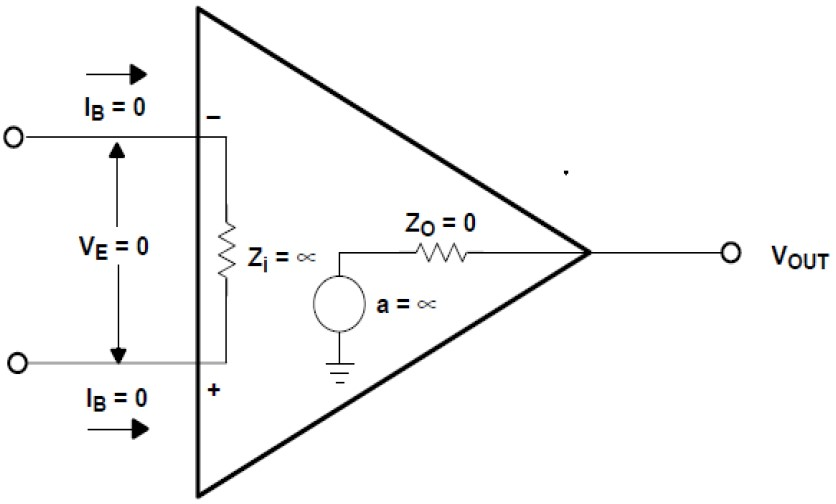
\includegraphics[width=0.7\columnwidth]{images/OPV_1.jpg} 		
	\end{center}
\end{minipage}
\hfill
\begin{minipage}{0.38\columnwidth}
	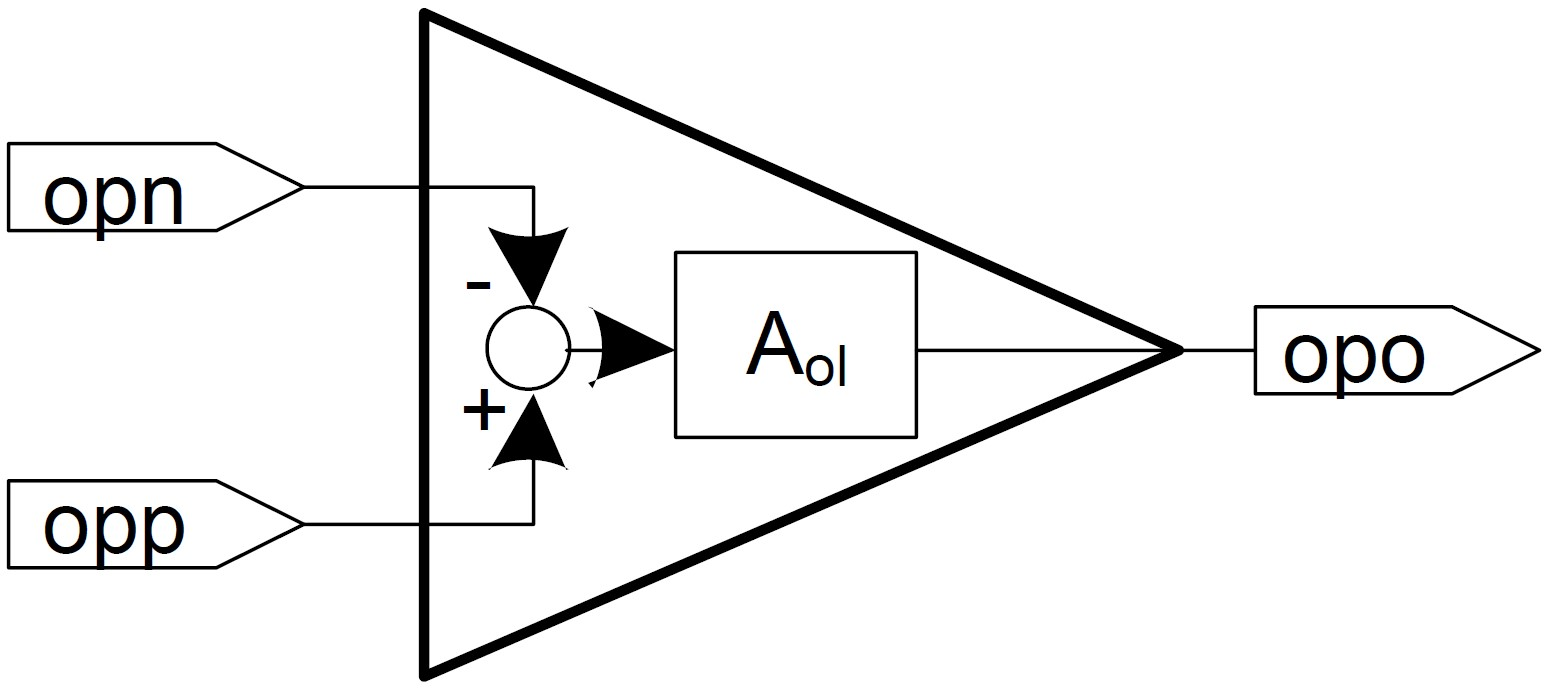
\includegraphics[width=0.8\columnwidth]{images/OPV_2.jpg} 
\end{minipage}


\subsection{OpAmp als Verstärker}

\begin{itemize}
	\item \textbf{Rückkopplung auf negativen Eingang}
	\item OpAmp stellt $V_{\rm out}$ so ein, dass beide Eingänge die gleiche Spannung aufweisen\\
		\textrightarrow\ $V_{\rm opn} = V_{\rm opp}$
	\item \textbf{opn ist virtueller Massepunkt}
	\item Lineare Schaltung (solange nicht am Anschlag) \textrightarrow\ Superposition
	\item \cbl{für $A_{\rm ol} \neq \infty$} $V_{\rm opn}$ als Spannungsteiler von $V_{\rm out}$ zu ausgeschaltetem $V_{in_i}$ durch \\
		Superposition  ausdrücken
\end{itemize}


\begin{minipage}[c]{0.48\columnwidth}
	$$ V_{\rm out} = A_{\rm ol} \cdot (V_{\rm opp} - V_{\rm opn}) $$
\end{minipage}
\hfill
\begin{minipage}[c]{0.48\columnwidth}
	$$ V_{\rm out} = A_{\rm ol} \cdot (V_{\rm in} + V_{\rm os} - V_{\rm opn} ) $$ 
\end{minipage}


\subsection{Grundschaltungen OpAmp}

\subsubsection{Nicht-Invertierender Verstärker}

\begin{minipage}[c]{0.4\columnwidth}
	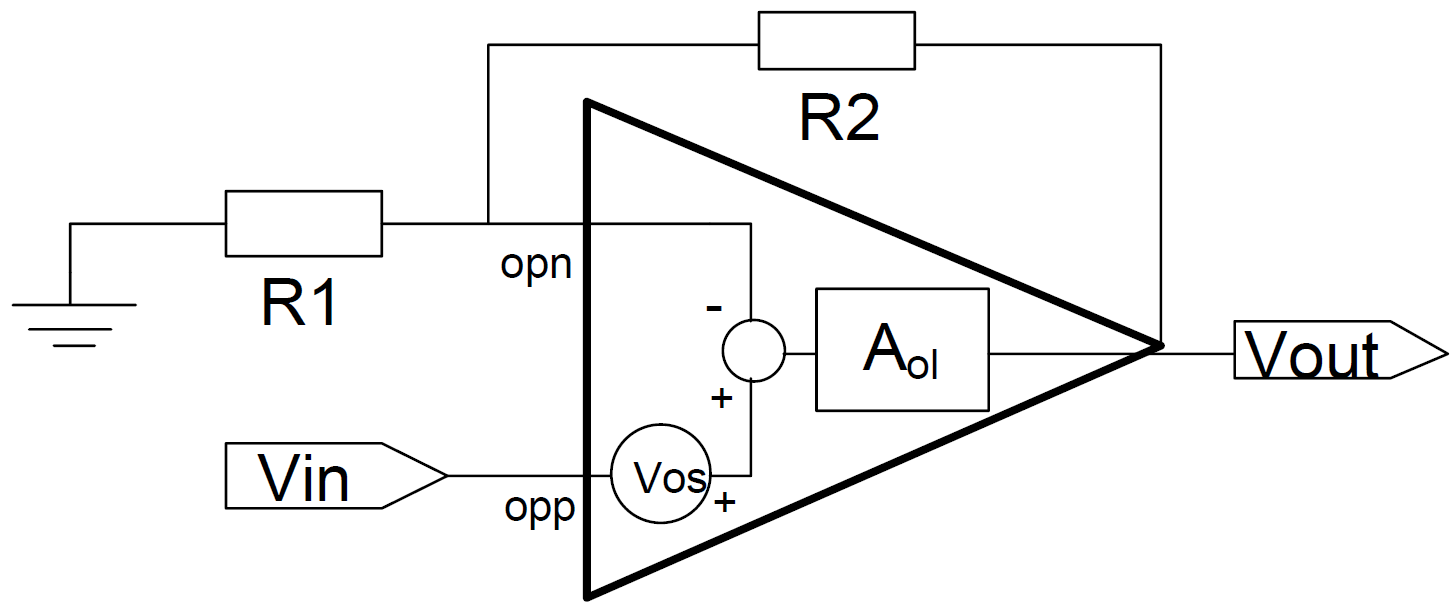
\includegraphics[width=\columnwidth]{images/nicht-invertierender_verstaerker_offset.png}
\end{minipage}
\hfill
\begin{minipage}[c]{0.58\columnwidth}
	$$ V_{\rm opn} = (V_{\rm GND} + V_{\rm os}) \cdot \frac{R_2}{R_1 + R_2} + \frac{R_1}{R_1 + R_2} \cdot V_{\rm out} $$ 
\end{minipage}


\begin{minipage}[t]{0.48\columnwidth}
	\textbf{Real}

	\vspace{0.1cm}

	\scalebox{0.8}{
	$ \boxed {\quad  V_{\rm out} = \frac{A_{\rm ol}}{1 + A_{\rm ol} \cdot \frac{R_1}{R_1 + R_2}} \cdot (V_{\rm in} + V_{\rm os}) - \frac{R_2}{R_1} \cdot A_{\rm GND} } $}
\end{minipage}
\hfill
\begin{minipage}[t]{0.5\columnwidth}
	\textbf{Ideal}

	\vspace{0.1cm}

	\scalebox{0.9}{
	$ \boxed { \quad V_{\rm out} = ( V_{\rm in} + V_{\rm os}) \cdot \frac{R_1 + R_2}{R_1} - \frac{R_2}{R_1} \cdot A_{\rm GND} } $}
\end{minipage}


\subsubsection{Invertierender Verstärker}

\begin{minipage}[c]{0.4\columnwidth}
	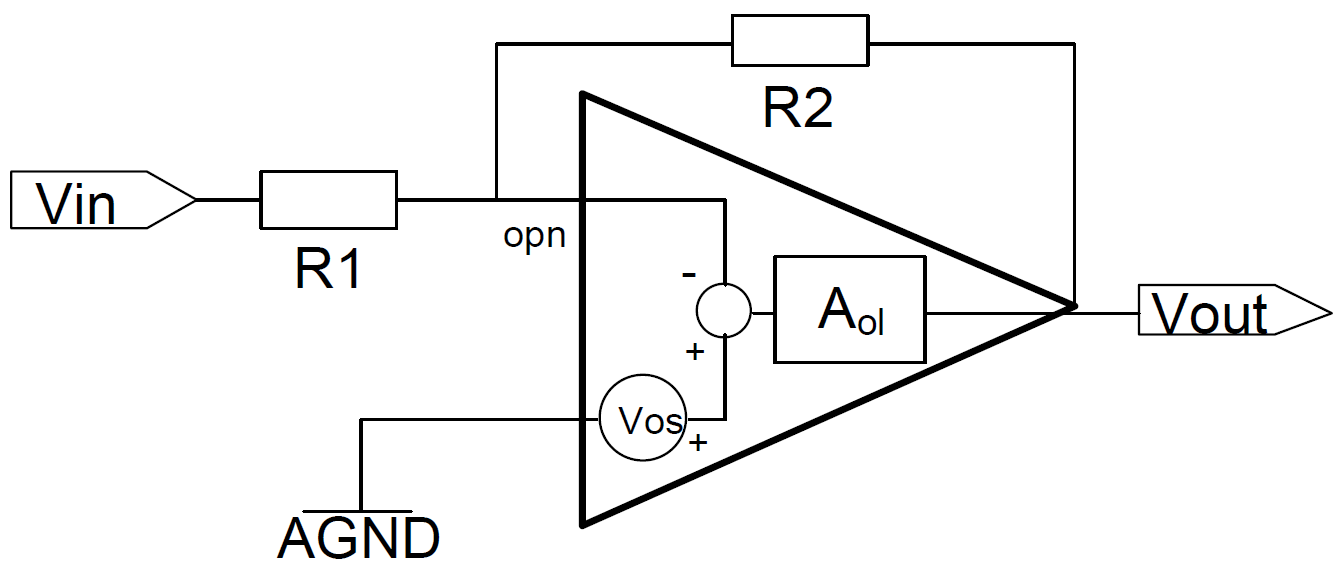
\includegraphics[width=0.9\columnwidth]{images/invertierender_verstaerker_offset.png}
\end{minipage}
\hfill
\begin{minipage}[c]{0.58\columnwidth}
	Knoten: $I_2 - I_1 - I_{\rm opn} = 0$ mit $I_{\rm opn} = 0$: \quad  $I_2 = I_1$ 
	$$ I_1 = - \frac{V_{\rm in}}{R_1} \qquad V_{\rm out} = V_{R_2} = I_2 \cdot R_2 = I_1 \cdot R_2 $$
	$$ \boxed{ V_{\rm opn} = V_{\rm in} \cdot \frac{R_2}{R_1 + R_2} + V_{\rm out} \frac{R_1}{R_1 + R_2}} $$
\end{minipage}

\vspace{0.2cm}

\begin{minipage}[t]{0.54\columnwidth}
	\textbf{Real}

	\vspace{0.1cm}

	\scalebox{0.8}{
	% $ \boxed{ V_{\rm out} = \frac{A_{\rm ol}}{1+A_{\rm ol} \cdot \frac{R_1}{R_1 + R_2}} \cdot \Big( A_{\rm GND} + V_{\rm os} \Big) - V_{\rm in} \cdot \frac{R_2}{R_1}  } $
	$ \boxed{ V_{\rm out} = \frac{(R_1 + R_2) \cdot A_{\rm ol} \cdot (V_{\rm pos} + V_{\rm os}) - R_2 \cdot A_{\rm ol} \cdot V_{\rm neg} }{R_1 + R_2 +  R_1 \cdot A_{\rm ol}} }$
	}
\end{minipage}
\hfill
\begin{minipage}[t]{0.44\columnwidth}
	\textbf{Ideal}

	\vspace{0.1cm}

	\scalebox{0.8}{
	$ \boxed{ V_{\rm out} = \frac{R_1 + R_2}{R_1} \cdot \Big(  A_{\rm GND} + V_{\rm os} \Big) - V_{\rm in} \cdot \frac{R_2}{R_1} } $ }
\end{minipage}


\subsubsection{Invertierender Summierender Verstärker (Addierer)}

\begin{minipage}[c]{0.38\columnwidth}
	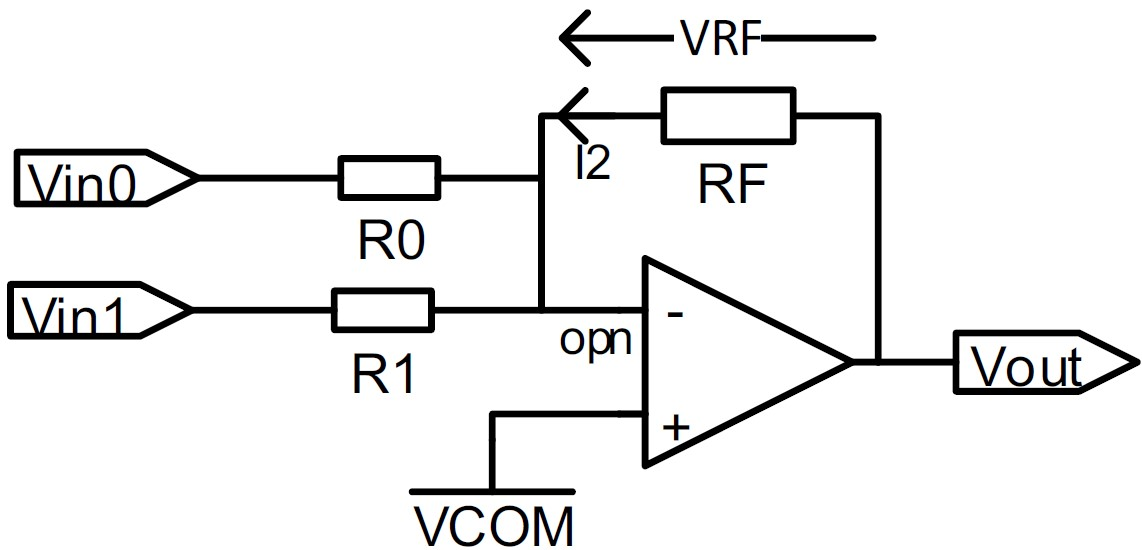
\includegraphics[width=\columnwidth]{images/invertierender_summierender_verstaerker.jpg}
\end{minipage}
\hfill
\begin{minipage}[c]{0.58\columnwidth}
	$$ I_2 - I_1 - I_0 = 0 \text{ \textrightarrow\ } I_2 = -I_1 - I_0 $$
	$$ I_0 = \frac{V_{\rm in0} - V_{\rm COM} - V_{\rm os}}{R_0} \quad I_1 = \frac{V_{in1} - V_{COM}- V_{\rm os}}{R_1} $$
\end{minipage}

\vspace{0.2cm}

$$ \boxed{ V_{\rm out} = (V_{\rm COM} + V_{\rm os}) \cdot \Bigg( \frac{R_f + R_0 || R_1}{R_0 || R_1} \Bigg)  - R_F \cdot \Bigg( \frac{V_{\rm in0}}{R_0} + \frac{V_{\rm in1}}{R_1} \Bigg) } $$


\subsubsection{Buffer}

\begin{minipage}[c]{0.48\columnwidth}
	\begin{center}
		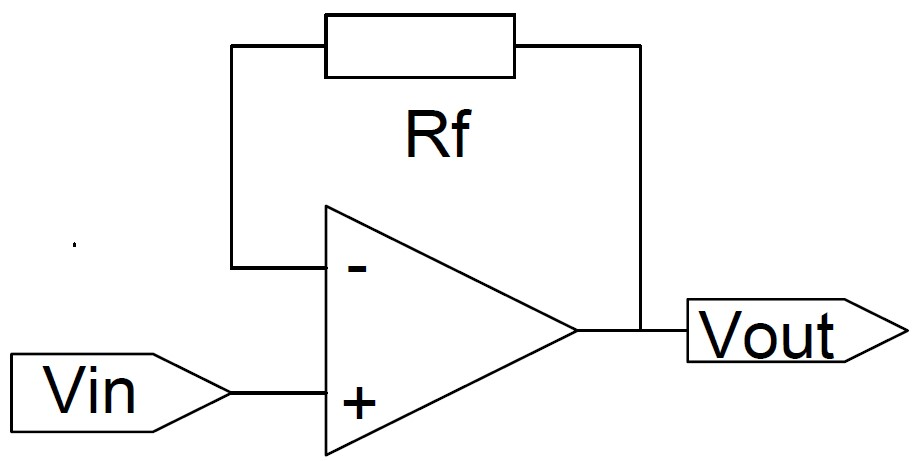
\includegraphics[width=0.65\columnwidth]{images/buffer_1.jpg}

		\begin{itemize}
			\item $V_{\rm out} = V_{\rm in} + V_{\rm os}$
			\item Keine Belastung an $V_{\rm in}$
		\end{itemize}
	\end{center}
\end{minipage}
\hfill
\begin{minipage}[c]{0.48\columnwidth}
	\begin{center}
		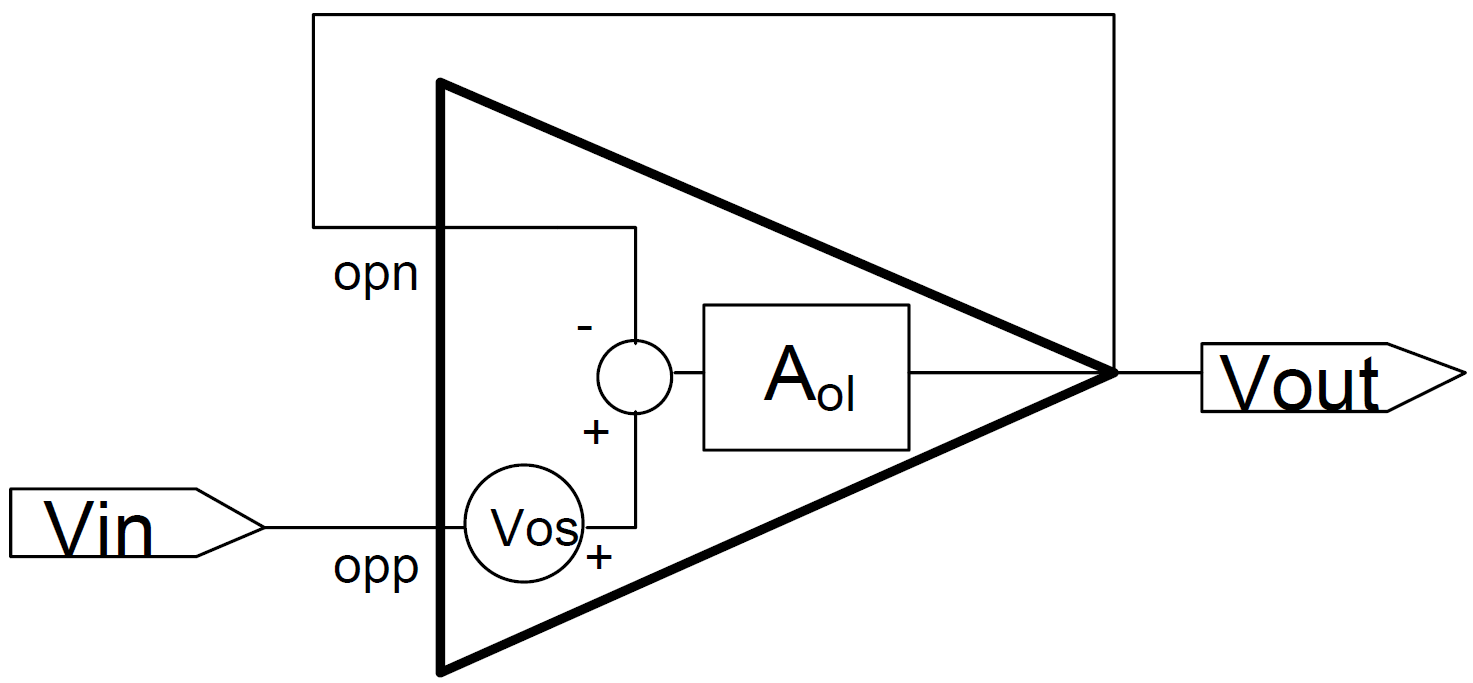
\includegraphics[width=0.7\columnwidth]{images/buffer_offset.png}

		\begin{itemize}
			\item Kopplungsfaktoren $= 1$
			\item Tiefer Ausgangswiderstand
		\end{itemize}
	\end{center}
\end{minipage}


\subsection{Analoge Rechenschaltungen mit OpAmps}

\subsubsection{Differenzverstärker (Gewichteter Subtrahierer)}

\begin{minipage}[c]{0.4\columnwidth}
	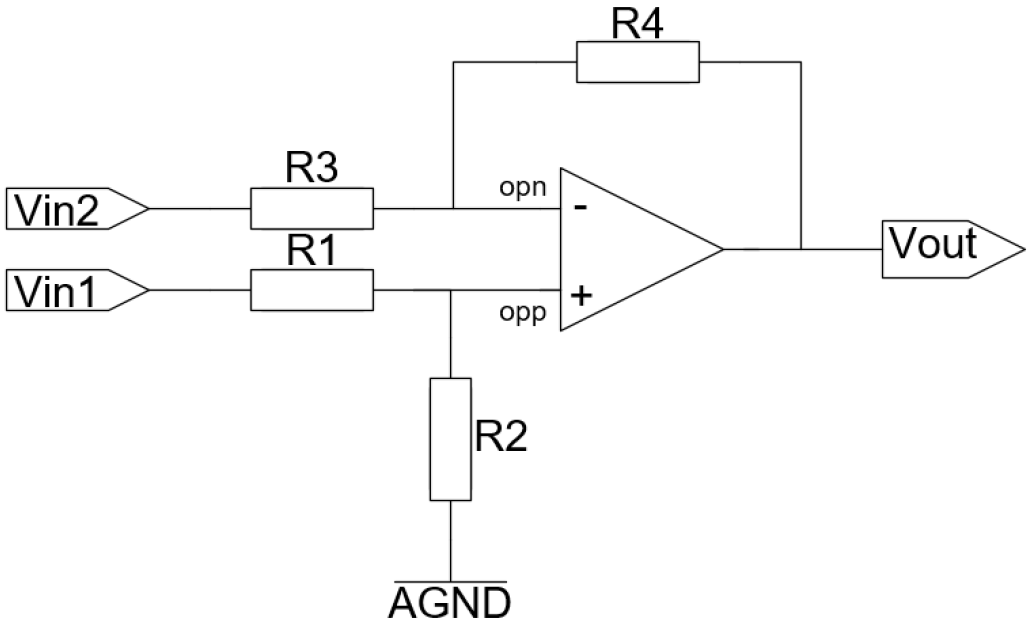
\includegraphics[width=\columnwidth]{images/differenzverstärker.png}
\end{minipage}
\hfill
\begin{minipage}[c]{0.58\columnwidth}
	\begin{tabular}{ll}
		oben:	& invertierender Verstärker			\\
		unten: 	& nicht-invertierender Verstärker 	\\
				& mit Spannungsteiler
	\end{tabular}
\end{minipage}

$$ \boxed{  V_{\rm out} = \frac{R_3 + R_4}{R_3} \cdot \Bigg( \frac{R_1}{R_1 + R_2} \cdot A_{\rm GND} + \frac{R_2}{R_1 + R_2} \cdot V_{\rm in1} \Bigg) - \frac{R_4}{R_3} \cdot V_{\rm in2} } $$
$$ \boxed{ \text{Für } R_1 = R_3, \, R_2 = R_4: \quad  V_{\rm out} =  A_{\rm GND} + \frac{R_4}{R_3} \cdot ( V_{\rm in1} - V_{\rm in2}) } $$


\subsubsection{Instrumentenverstärker}

OP1 und OP2 sind nicht-invertierende Verstärker mit gemeinsamem Widerstand $R_g$

\begin{minipage}[c]{0.5\columnwidth}
	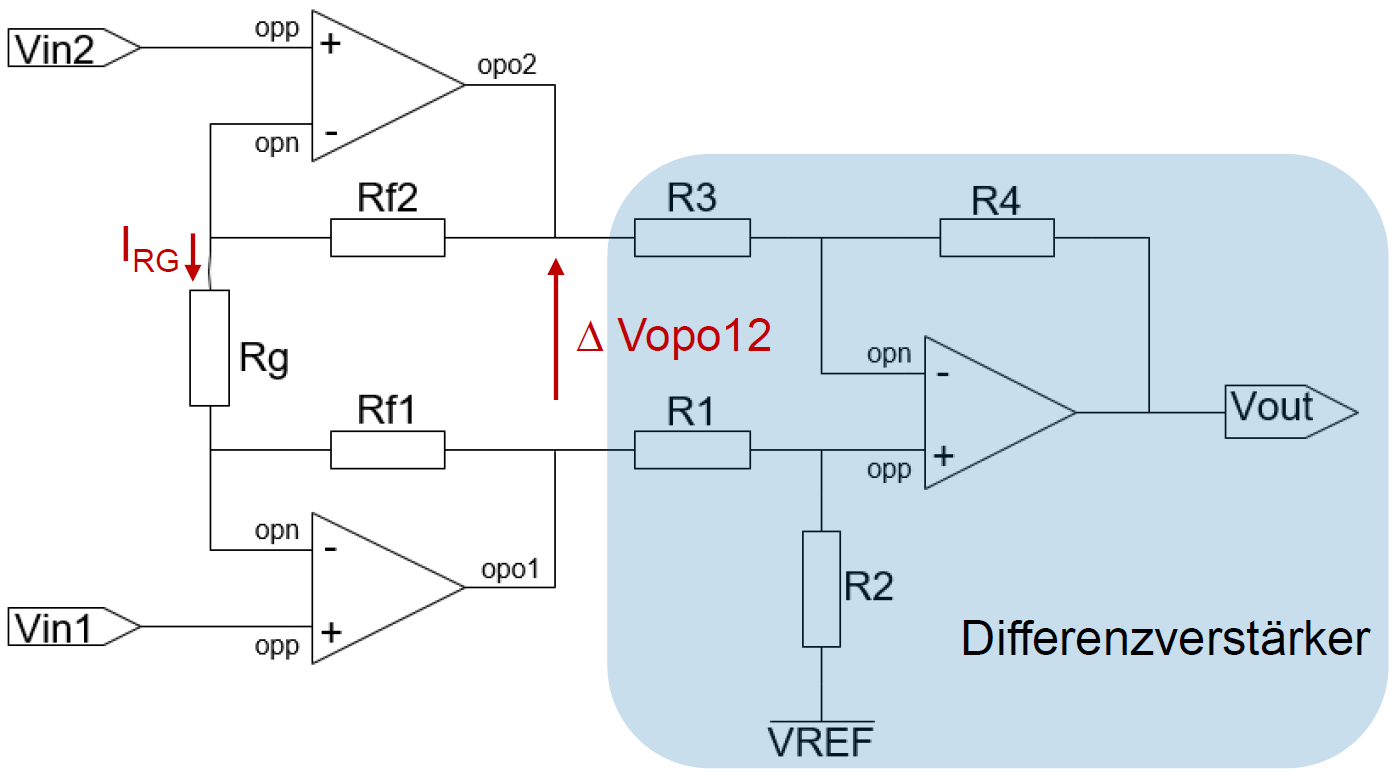
\includegraphics[width=\columnwidth]{images/instrumentenverstaerker.png}
\end{minipage}
\hfill
\begin{minipage}[c]{0.48\columnwidth}
	$$ I_{\rm Rg} = \frac{V_{\rm in2} - V_{\rm in1}}{R_g} $$
	$$ V_{\rm opo2} = V_{\rm in2} + \frac{R_{f2}}{R_g} \cdot(V_{\rm in2} - V_{\rm in1}) $$
	$$ V_{\rm opo1} = V_{\rm in1} + \frac{R_{f1}}{R_g} \cdot(V_{\rm in1} - V_{\rm in2}) $$
\end{minipage}

$$ \boxed{ \Delta V_{\rm opo12} = V_{\rm opo2} - V_{\rm opo1} = \Bigg( 1 + \frac{R_{f1} + R_{f2}}{R_g} \Bigg) \cdot(V_{\rm in1} - V_{\rm in2}) } $$
$$ \boxed{ \text{Für } R_1 = R_3, \, R_2 = R_4: \quad  V_{\rm out} =  V_{\rm REF} + \frac{R_4}{R_3} \cdot \Bigg( 1 + \frac{R_{f1} + R_{f2}}{R_g} \Bigg) \cdot(V_{\rm in1} - V_{\rm in2}) } $$


\columnbreak


\subsection{Mehrstufige Verstärker}

Für $\mathrm{AGND} \neq 0 \, \volt$ muss Superposition angewendet werden. \\
\textrightarrow\ $\mathrm{AGND}$ als Quelle annehmen und anderen Eingang 'ausschalten'

\begin{center}
	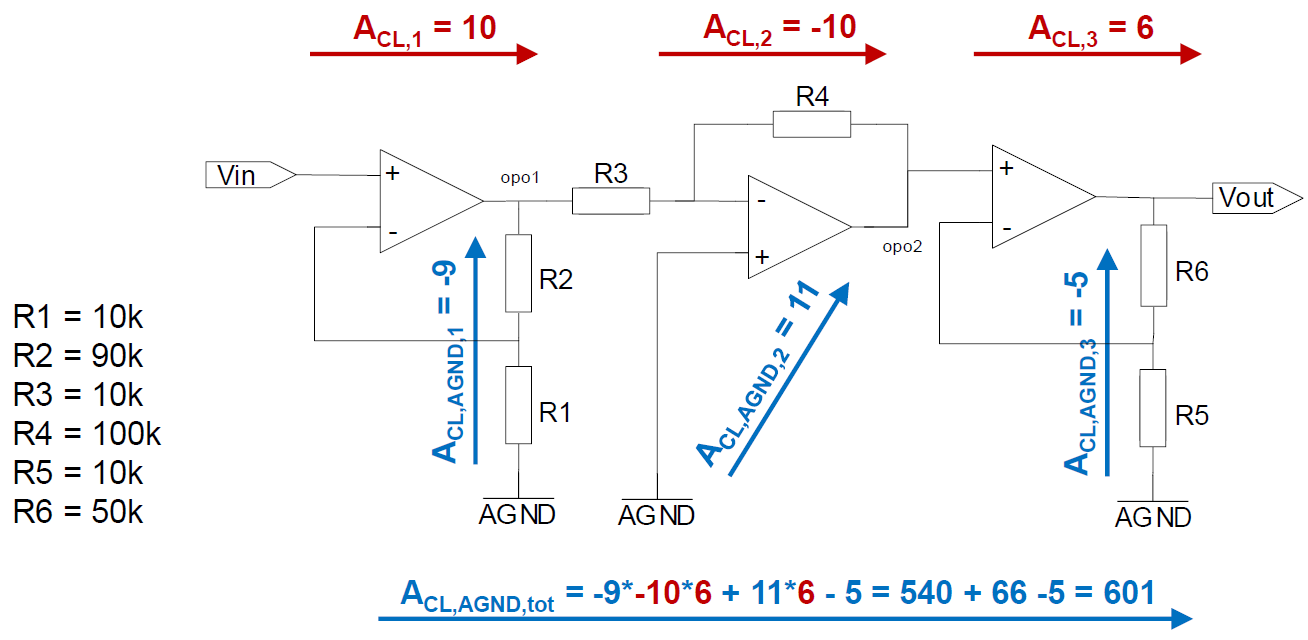
\includegraphics[width=0.85\columnwidth]{images/mehrstufige_verstaerker.png}
\end{center}


\subsection{Gesteuerte Quellen}

\subsubsection{Stromgesteuerte Stromquellen}

\begin{minipage}[c]{0.4\columnwidth}
	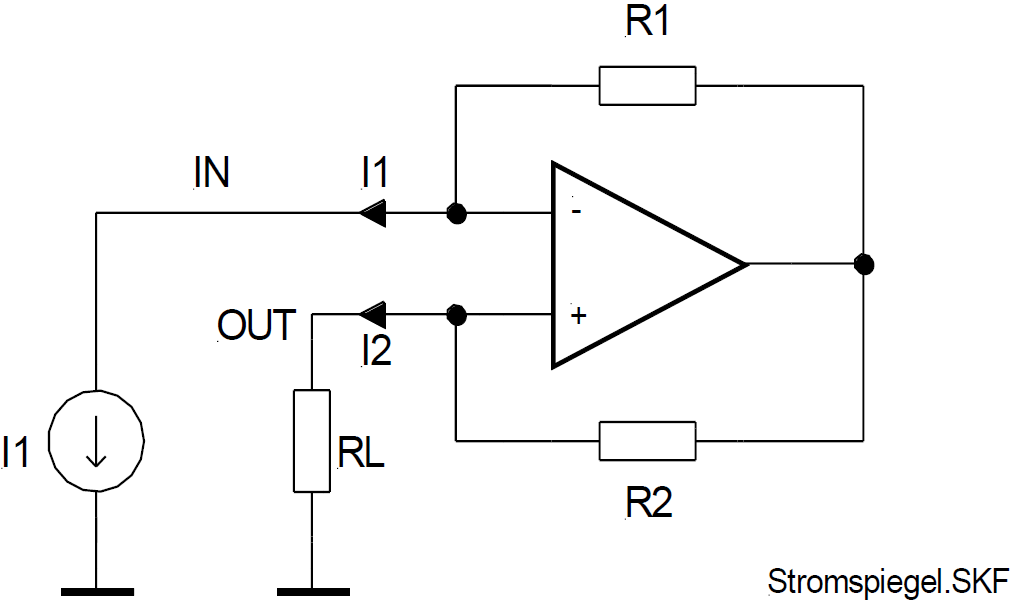
\includegraphics[width=\columnwidth]{images/stromspiegel_OPV.png}
\end{minipage}
\hfill
\begin{minipage}[c]{0.48\columnwidth}
	$$ V_{R1} = V_{R2} \qquad R_1 \, I_1 = R_2 \, I_2 $$
	$$ \boxed{ A_i = \frac{I_2}{I_1} = \frac{R_1}{R_2} }$$
\end{minipage}


\subsubsection{Spannungsgesteuerte Stromquellen}

\begin{minipage}[c]{0.4\columnwidth}
	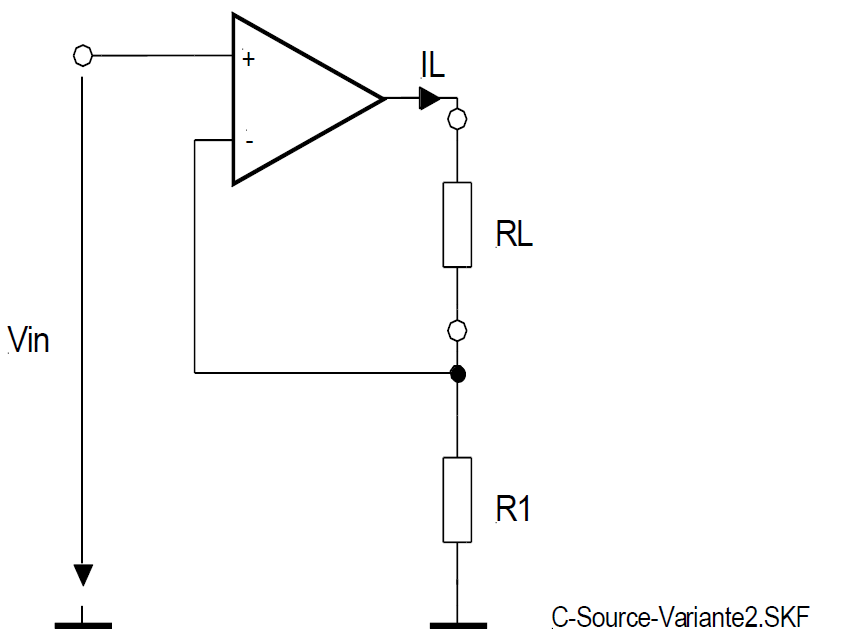
\includegraphics[width=\columnwidth]{images/spannungsgesteuerte_stromquelle_V1.png}
	$$ I_L = \frac{V_{\rm in}}{R_1}$$
	Nachteil: Last muss 'floating' sein
\end{minipage}
\hfill
\begin{minipage}[c]{0.48\columnwidth}
	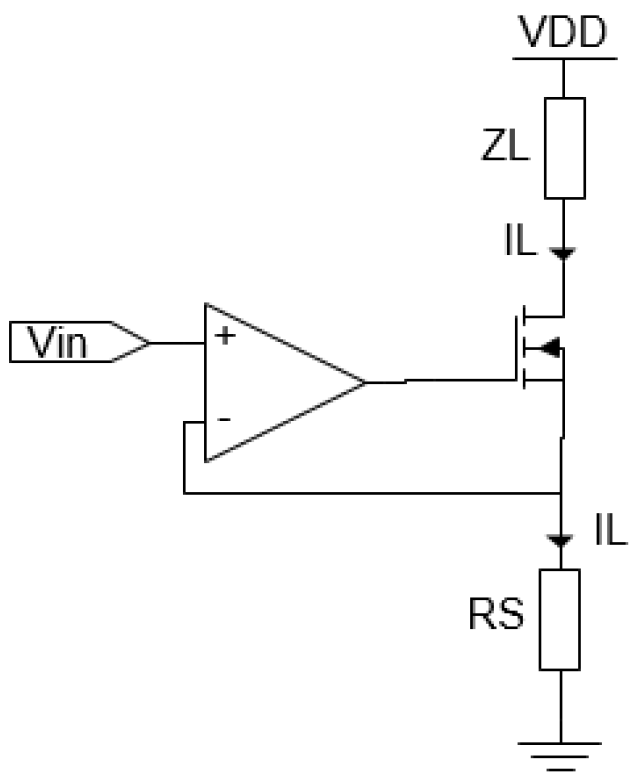
\includegraphics[width=0.6\columnwidth]{images/spannungsgesteuerte_stromquelle_V2.png}
	$$ I_L = \frac{V_{\rm in}}{R_s}$$
\end{minipage}


\subsection{Einfache Filterschaltungen mit OpAmps}

\subsubsection{Integratoren}

\begin{tabular}{ll}
	RL-Integrator:	& Spulen sind nichtideal und teuer 		\\
					& Spulen erzeugen oft Oszillationen 	\\
	RC-Integrator: 	& fast immer für aktive Filter verwendet
\end{tabular}

\vspace{0.2cm}

\begin{minipage}[c]{0.4\columnwidth}
	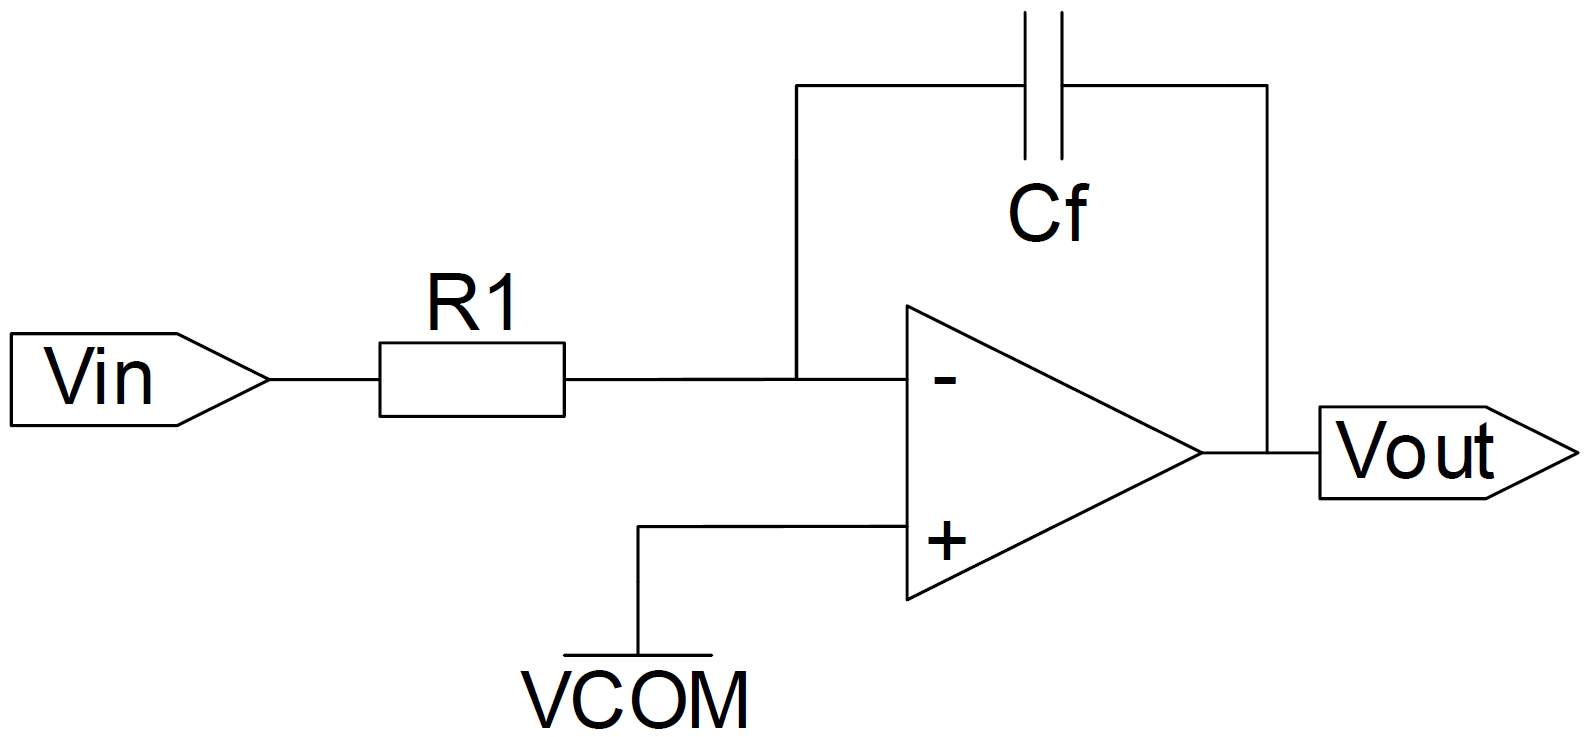
\includegraphics[width=\columnwidth]{images/integrator.png} 
\end{minipage}
\hfill
\begin{minipage}[c]{0.58\columnwidth}
	$$ \boxed{ V_{\rm out}(t) = - \frac{1}{R_1 \cdot C_f} \int\limits_0^t V_{\rm in}(\tau) \, \diff \tau + V_{C_f}(0) } $$
	$$ \boxed{ V_{\rm out}(t) = - \frac{1}{C_f} \int\limits_0^t I_{C_f}(\tau) \, \diff \tau + V_{C_f}(0) } $$
\end{minipage}


\subsubsection{Differenzierer}

\begin{minipage}[c]{0.4\columnwidth}
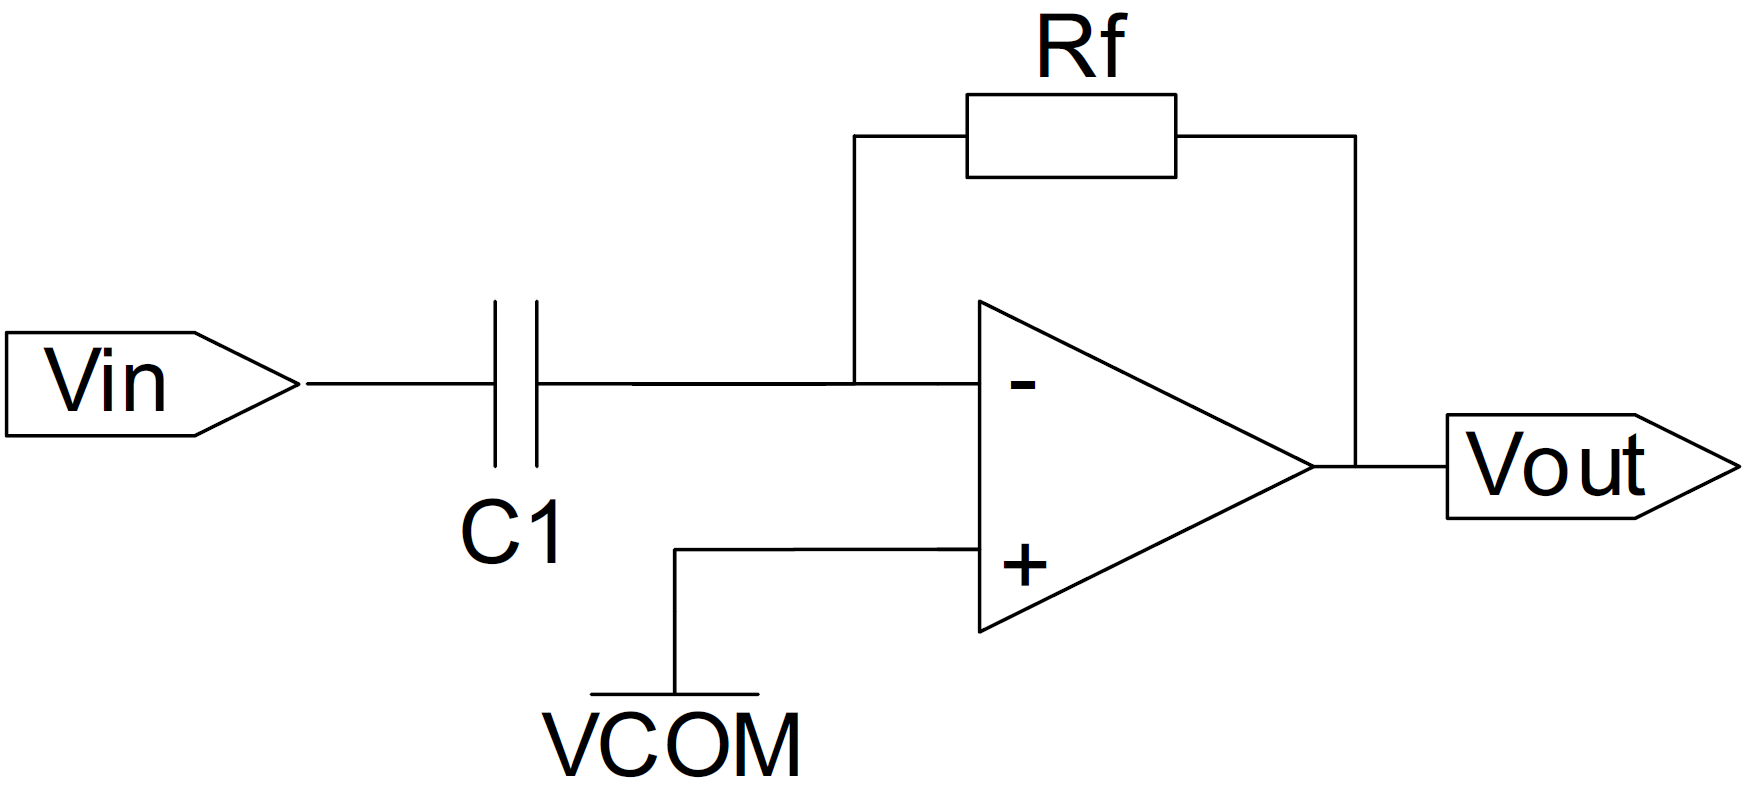
\includegraphics[width=\columnwidth]{images/differenzierer.png}
\end{minipage}
\hfill
\begin{minipage}[c]{0.58\columnwidth}
	$$ \boxed{ V_{\rm out} = - R_f \cdot C_1 \frac{\diff V_{\rm in}}{\diff t} } $$
	$$ \boxed{ i_{c} = C_1 \frac{\diff v_c}{\diff t} = C_1 \frac{\diff V_{\rm in}}{\diff t} } $$
\end{minipage}

\vspace{0.2cm}

\myul{\textbf{Differenzierer im Frequenzbereich}}

\vspace{0.1cm}

\begin{itemize}
	\item Hohe Freqeunzen werden mehr verstärkt
	\item Rückkopplungsfunktion ist Tiefpass
	\item Realer OpAmp bildet auch Tiefpass
	\item Beide Tiefpasse erzeugen zusammen $180 \, \degree$ Phasenschiebung \\
		\textrightarrow\ Mitkopplung \textrightarrow\ Schwingung 
	\item Kleines $C$ parallel zu $R_f$ unterdrückt Schwingungen
\end{itemize}


\subsubsection{Tiefpass}

\begin{minipage}[c]{0.4\columnwidth}
	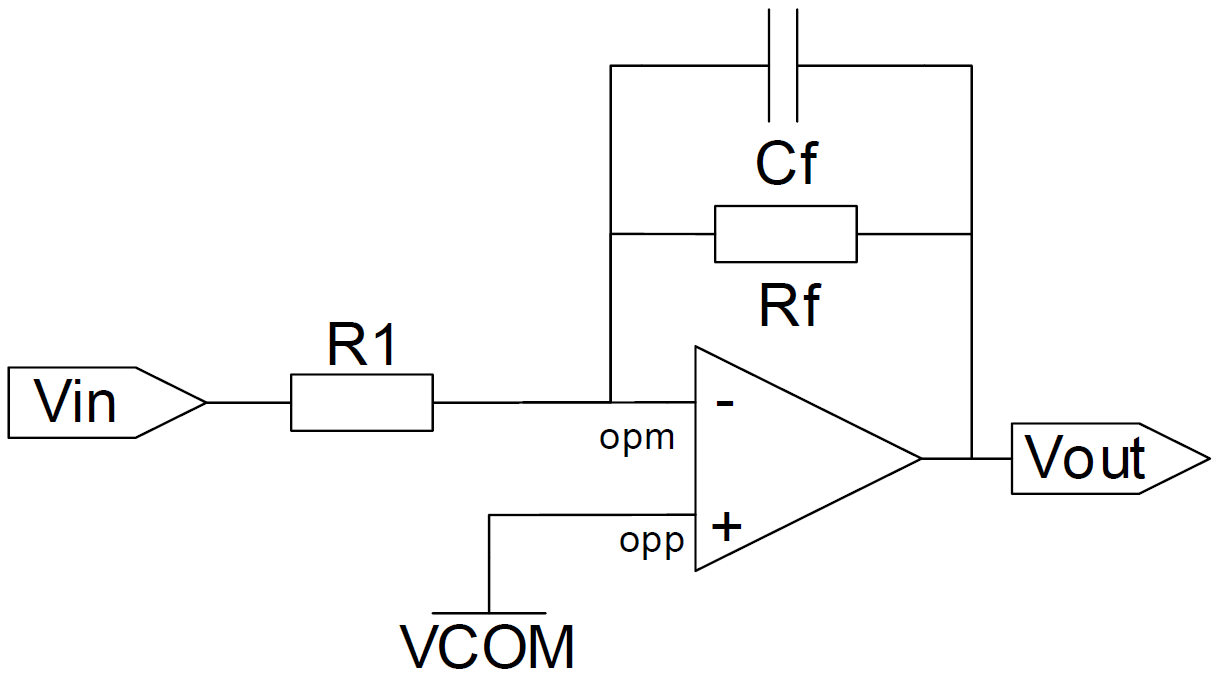
\includegraphics[width=\columnwidth]{images/tiefpass.png}
\end{minipage}
\hfill
\begin{minipage}[c]{0.58\columnwidth}
	\begin{tabular}{ll}
		\cbl{Tiefe $f$}:  	& $R_f$ limitiert Verstärkung 	\\
							& $I_{C_f} = 0$ (Unterbruch) 	\\
		\cgn{Hohe $f$}:		& $-20 \, \deci \bel$ / Dek
	\end{tabular}

	$$ \cbl{ \boxed{ V_{\rm out} = - \frac{R_f}{R_1} \cdot V_{\rm in} } } \qquad \cgn{ \boxed{ f_g = \frac{1}{2 \, \pi \cdot R_f \cdot C_1} } } $$
\end{minipage}


\subsubsection{Bandpass}

\begin{minipage}[c]{0.48\columnwidth}
	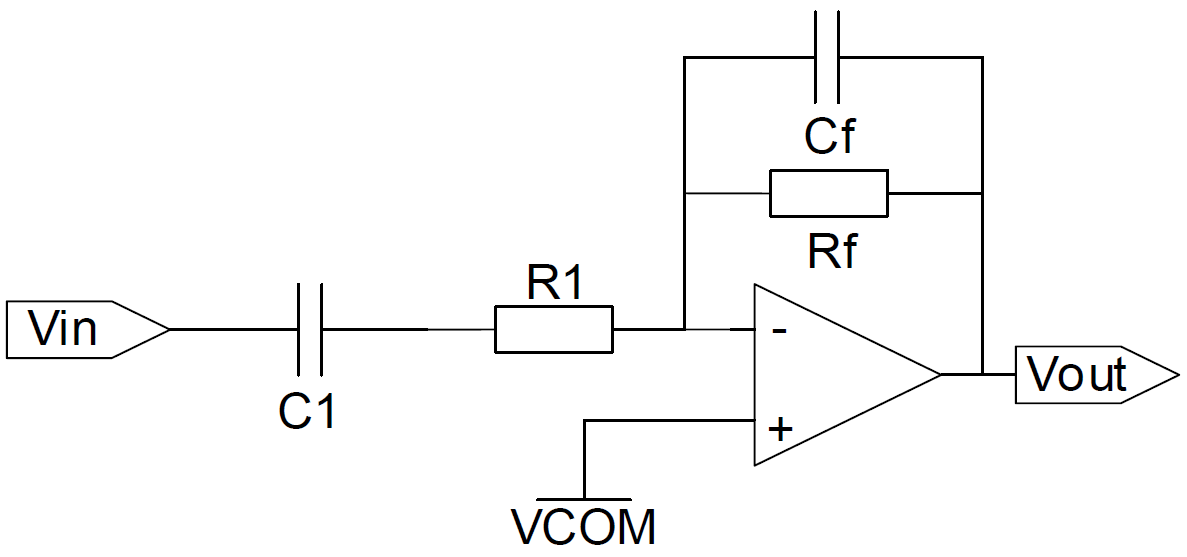
\includegraphics[width=\columnwidth]{images/bandpass.png} 
\end{minipage}
\hfill
\begin{minipage} [c]{0.48\columnwidth}
	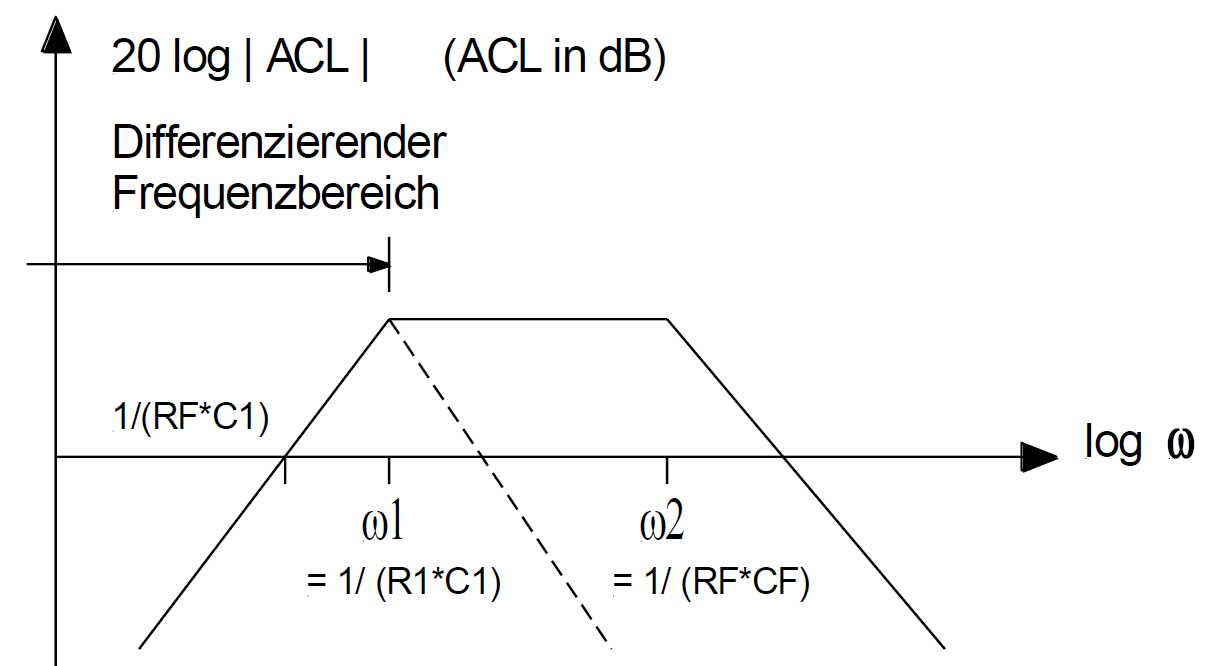
\includegraphics[width=\columnwidth]{images/bandpass_amplitudengang.png}
\end{minipage}

\vspace{0.2cm}

\begin{tabular}{ll}
	$R_1$ & limitiert Eingangsstrom 						\\
	$C_f$ & limitiert $V_{\rm out}$ bei hohen Frequenzen 
\end{tabular}


\subsubsection{Allpass}

\begin{itemize}
	\item Betrag der Verstärkung $= 1$ ($-1$ @ $180 \, \degree$ \textrightarrow\ $1$ @ $0 \, \degree$)
	\item Phase ändert mit der Frequenz von $180 \, \degree$ auf $0 \, \degree $
\end{itemize}

\vspace{0.2cm}

\begin{minipage}[c]{0.4\columnwidth}
	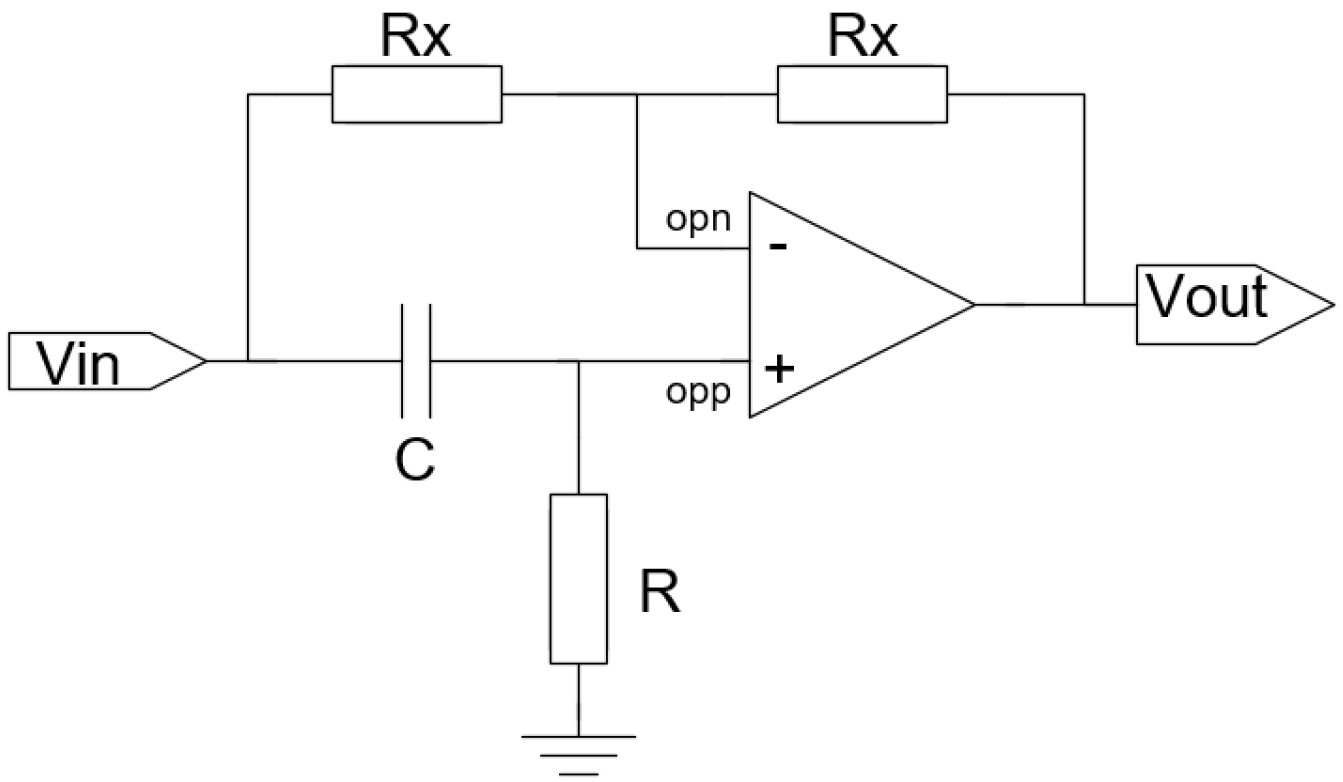
\includegraphics[width=\columnwidth]{images/allpass.png}
\end{minipage}
\hfill
\begin{minipage}[c]{0.58\columnwidth}
	\begin{tabular}{ll}
		\cbl{tiefe $f$}:	& $C$ sperrt (Unterbruch) 										\\
							& \textrightarrow\ $I_{C_f} = 0$  								\\
		\cgn{hohe $f$}: 	& $C$ ist Kurzschluss 											\\
							& $V_{\rm opn} = V_{\rm opp}$ \textrightarrow\ $I_{R_x} = 0$ 
	\end{tabular}

	$$ \cbl{ \boxed{ V_{\rm out} = - \frac{R_x}{R_x} \cdot V_{\rm in} = - V_{\rm in} } } \qquad 
	   \cgn{ \boxed{ V_{\rm out} = V_{\rm in} } } $$
\end{minipage}


\subsection{Nichtidealitäten von OpAmps}

\begin{tabular}{ll}
	\tabitem Endliche Verstärkung:	& $V_d = V_{\rm opp} - V_{\rm opn} = \frac{V_{\rm out}}{A_{\rm ol}}$	\\
	\tabitem Offset-Spannung:		& $V_{\rm os}$: Gleich verstärkt wie $V_{\rm opp}$
\end{tabular}


\subsubsection{Eingangsstromfehler - Bias-Strom $\rm{I_B}$}

\begin{minipage}[c]{0.48\columnwidth}
	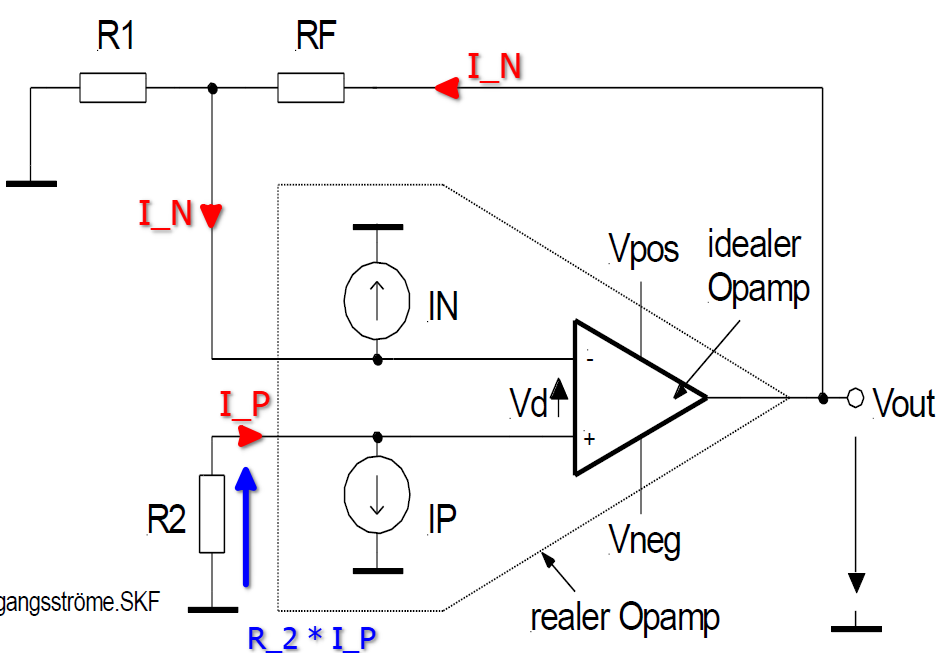
\includegraphics[width=\columnwidth]{images/bias-strom_grafik.png} 
\end{minipage}
\hfill
\begin{minipage}[c]{0.48\columnwidth}
	Modellierung durch Stromquellen \\
	$I_P$, $I_N$  

	\vspace{0.2cm}

	$V_{\rm outE} =$ Fehlerspannung aufgrund von $I_B, \, I_N$

	$$ I_B = \frac{I_P + I_N}{2} $$
\end{minipage}

\vspace{0.2cm}
$$ \boxed{ V_{\rm outE} = V_{\rm outE(N)} +  V_{\rm outE(P)} = I_N \, R_F - R_2 \, I_P \Bigg( \frac{R_F + R_1}{R_1}  \Bigg) } $$

$$ \text{Kompensation:} \quad I_B = \frac{I_P + I_N}{2}: \quad  V_{\rm outE} \overset{!}{=} 0 $$ 
$$ I_N = I_P: \quad R_F = R_2 \, \Bigg( \frac{R_F + R_1}{R_1} \Bigg) \quad \boxed{ R_2 = \frac{R_F \cdot R_1}{R_F + R_1} = R_F || R_1 } $$

\vspace{0.1cm}

\myul{\textbf{Bias-Strom-Kompensation mittels $\bm{R_2}$}}

\vspace{0.1cm}

\begin{minipage}[b]{0.3\columnwidth}
	\begin{center}
		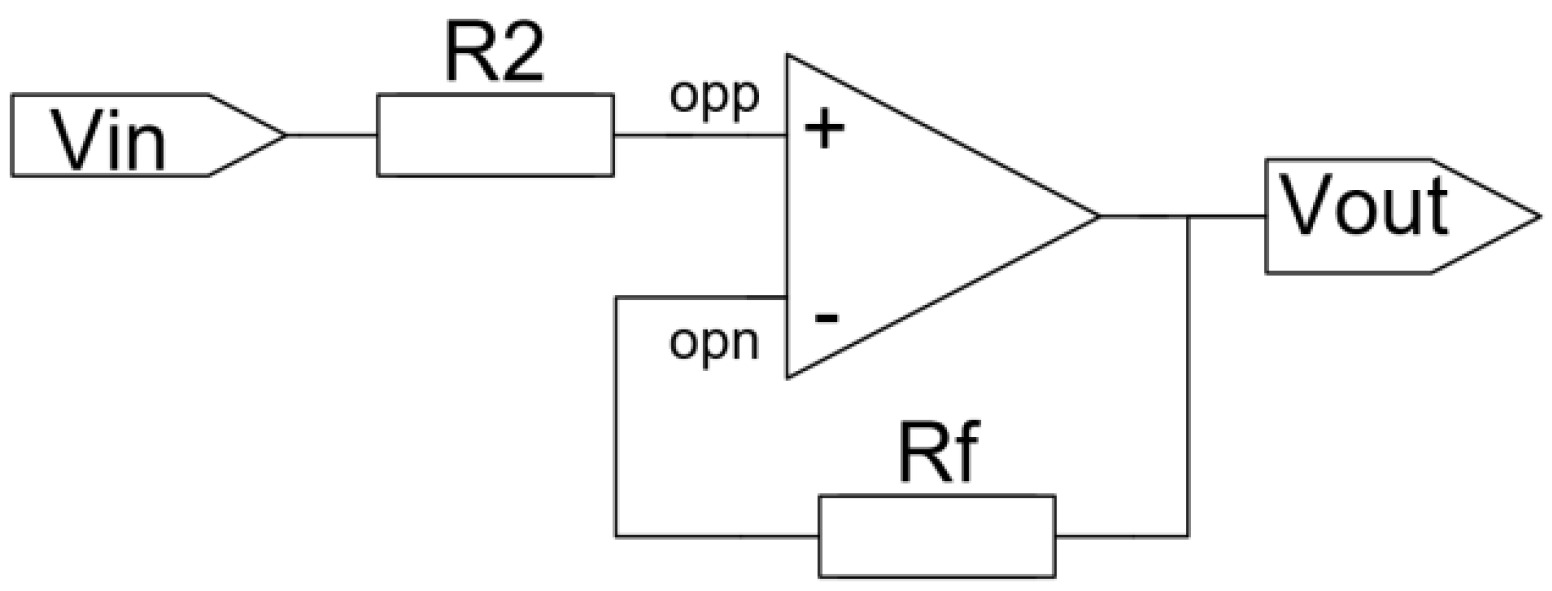
\includegraphics[width=\columnwidth]{images/kompensation_bias-strom_1.png}
		$$ R_2 = R_F $$
	\end{center}
\end{minipage}
\hfill
\begin{minipage}[b]{0.3\columnwidth}
	\begin{center}
		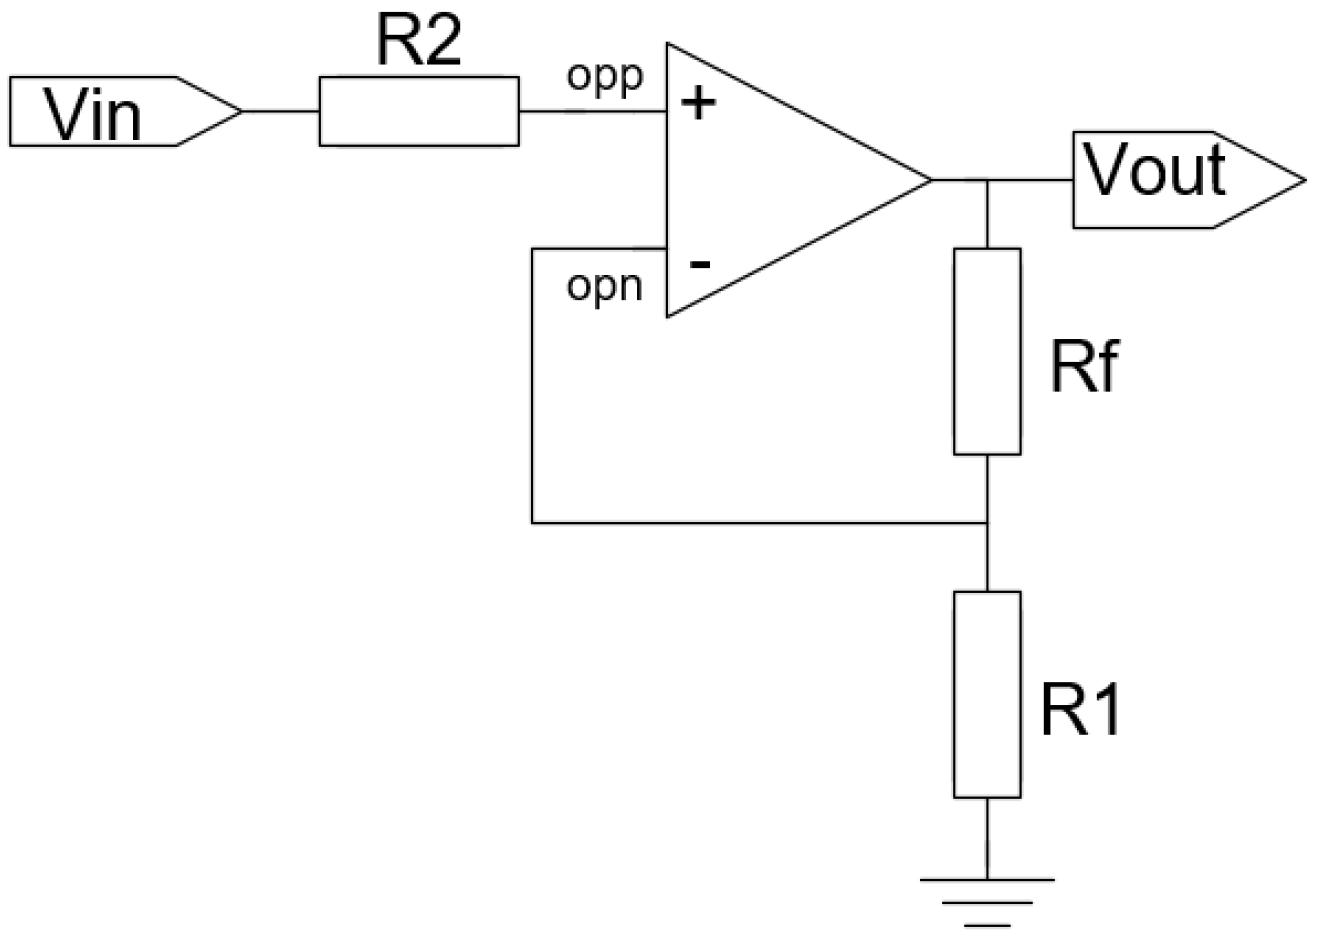
\includegraphics[width=\columnwidth]{images/kompensation_bias-strom_2.png}
		$$ R_2 = R_F || R_1 $$
	\end{center}
\end{minipage}
\hfill
\begin{minipage}[b]{0.3\columnwidth}
	\begin{center}
		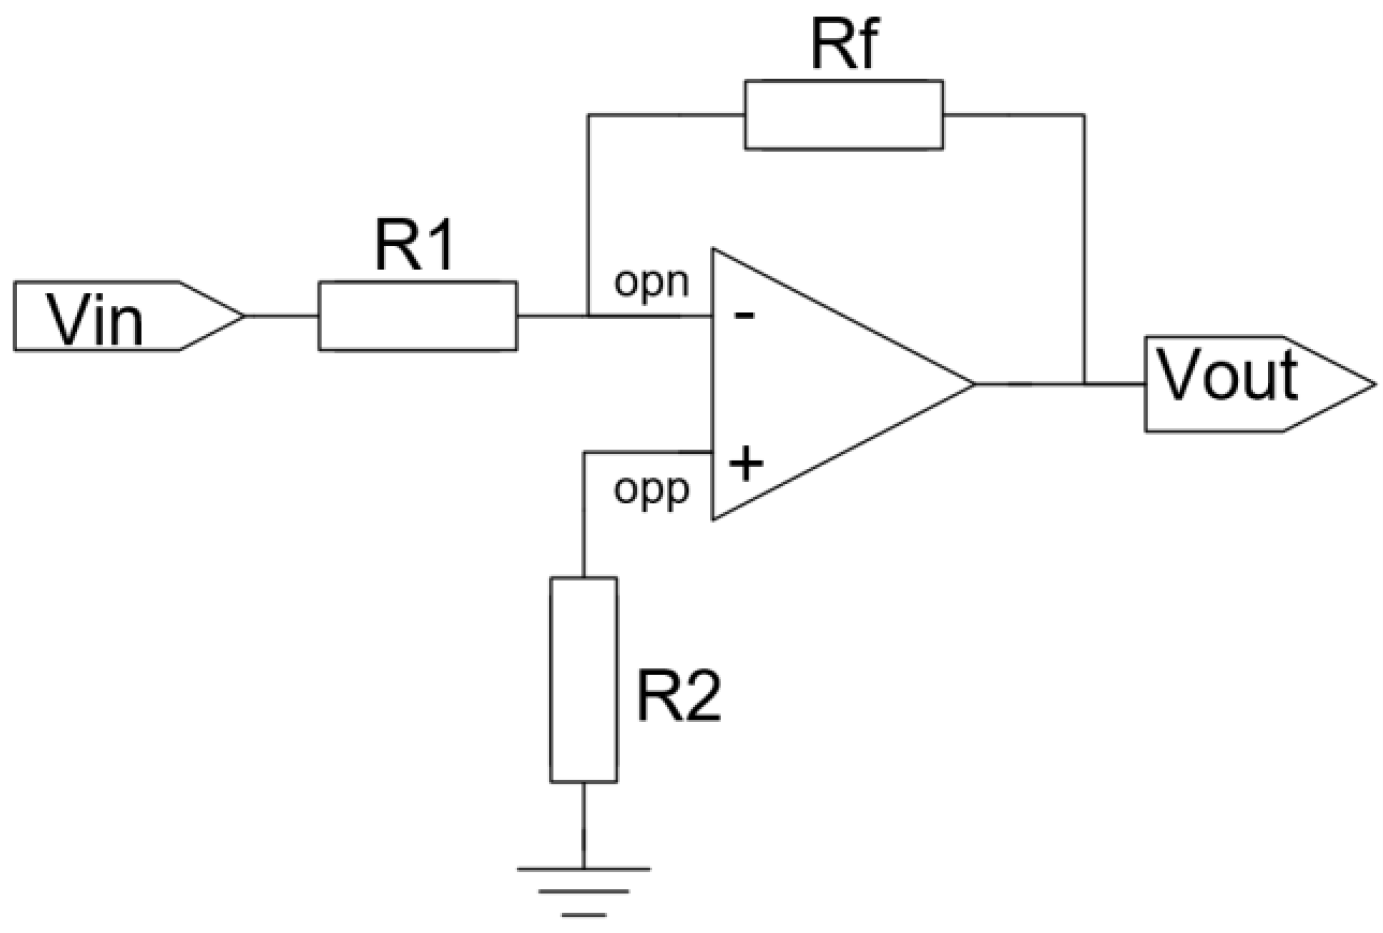
\includegraphics[width=\columnwidth]{images/kompensation_bias-strom_3.png}
		$$ R_2 = R_F || R_1 $$
	\end{center}
\end{minipage}


\subsubsection{Eingangsstromfehler - Offset-Strom $\bm{I_{\rm OS}}$}

Der Offset-Strom entsteht aufgrund von \textbf{Herstellungstoleranzen} und ist \textbf{nicht kompensierbar} 
$$ \text{Offset-Strom:} \quad I_{\rm OS} = I_P - I_N  $$

Wenn der Bias-Strom $I_B$ mittels $R_2$ kompensiert ist gilt: 

$$ \boxed{  V_{\rm outE} = R_F \cdot (I_N - I_P) = R_F \cdot I_{\rm OS} } $$

\textbf{ \textrightarrow\ Je kleiner $ \bm{R_F}$, desto kleiner die Fehlerspannung!}


\subsection{Dynamisches Verhalten von OpAmps}

\subsubsection{Verstärkungs-Bandbreite-Produkt (GB(W)P)}

\begin{minipage}[c]{0.45\columnwidth}
	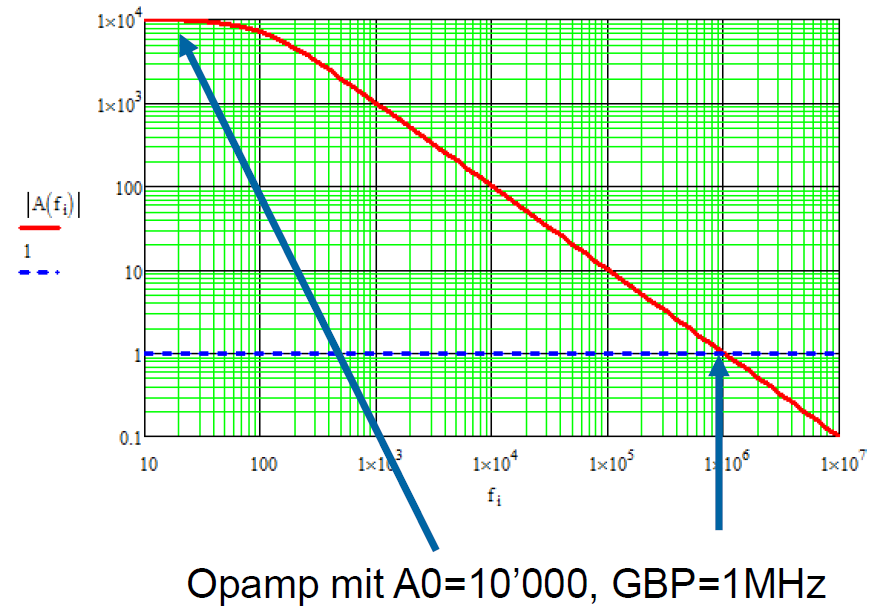
\includegraphics[width=\columnwidth]{images/verstaerkungs-bandbreite-produkt.png} 
\end{minipage}
\hfill
\begin{minipage}[c]{0.48\columnwidth}
	Verstärkung des OpAmps sinkt mit höherer Frequenz \\
	Datenblatt anstelle von $A_{\rm ol}$ (da Frequnzabhängig)

	$$ \boxed{ A_{\rm cl} \cdot f_{3 \deci \bel} = \mathrm{GBWP} = \const } $$
\end{minipage}


\subsubsection{Common Mode Rejection Ratio (CMRR)}

\begin{minipage}[c]{0.48\columnwidth}
	$$ \boxed{ \mathrm{CMRR} = \frac{\diff V_{\rm CM}}{\diff V_{\rm os}} }$$
\end{minipage}
\hfill
\begin{minipage}[c]{0.48\columnwidth}
	$$ \boxed{ V_{\rm CM} = \frac{V_{\rm opp} + V_{\rm opn}}{2} } $$
\end{minipage}


\subsubsection{Power Supply Noise Rejection Ratio (PSNRR)}

$$ \boxed{ \mathrm{PSNRR} = \frac{\diff V_{\rm supply}}{\diff V_{\rm os}} } $$


\subsection{Anstiegszeit (Slew-Rate)}

\begin{minipage}[c]{0.48\columnwidth}
	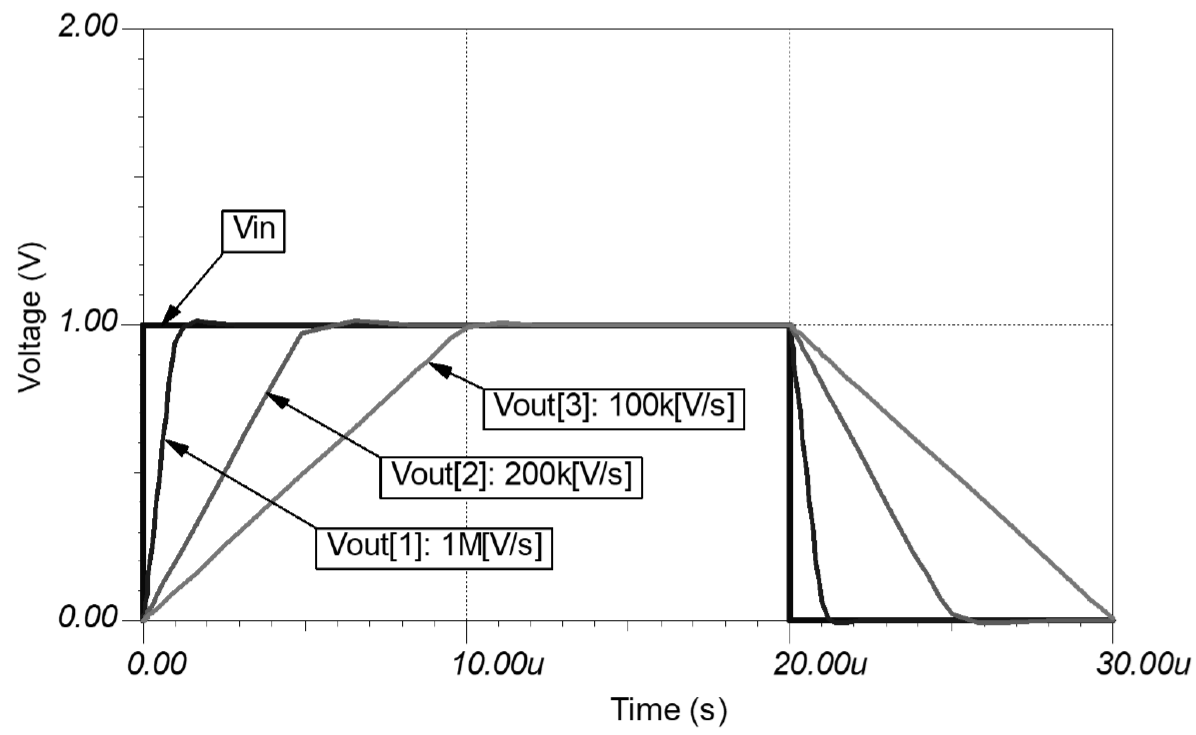
\includegraphics[width=\columnwidth]{images/slew_rate.png} 
\end{minipage}
\hfill
\begin{minipage}[c]{0.48\columnwidth}
	\raggedright
	Maximal mögliche Änderungsgeschwindigkeit der Ausgangsspannung des OpAmps

	$$ \boxed{ \mathrm{SR} = \Bigl| \frac{\diff V_{\rm out}}{\diff t} \Bigr|_{\rm max} } $$
\end{minipage}

Wenn der Ausgang schneller ändern soll als die Slew-Rate 'erlaubt', so wird das Ausgangssignal \textbf{begrenzt bzw. verformt} \\
\textrightarrow\ Signal verformt / Amplitude reduziert \textrightarrow\ Dreieck statt Sinus 
		\section{Komparatoren / Schmitt-Trigger}

\begin{itemize}
    \item OpAmp-Ausgang meistens am Anschlag $V_{\rm out_{max}}$ bzw. $V_{\rm out_{min}}$
    \item Rückkopplungsfrei oder Rückkopplung auf \textbf{positiven} Eingang
\end{itemize}

\vspace{0.2cm}

Schmitt-Trigger werden verwendet, wenn Signale \textbf{verrauscht} sind oder zur \textbf{Störungsunterdrückung} auf CLK-Signalen.


\subsection{OPV als Komparator}

\begin{minipage}[c]{0.4\columnwidth}
    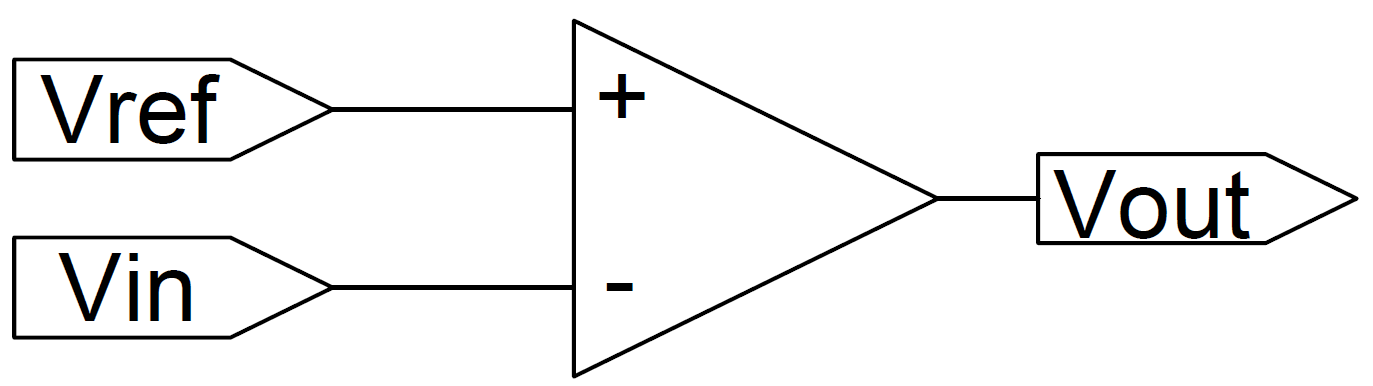
\includegraphics[width=\columnwidth]{images/komparator.png}
\end{minipage}
\hfill
\begin{minipage}[c]{0.48\columnwidth}
    Vergleicht $V_{\rm opp}$ mit $V_{\rm opn}$ bzw.$ V_{\rm ref}$ mit $V_{\rm in}$
\end{minipage}

\vspace{0.2cm}

\begin{itemize}
    \item Nur in sehr kleinem Bereich ist OpAmp in linearem Bereich
    \item Jeder OpAmp kann als Komparator eingesetzt werden
    \item Es gibt Komparatoren als spezialisierte Bausteile
    \item Komparatoren dürfen \textbf{nicht} als OpAmps eingesetzt werden
\end{itemize}


\subsection{Vergleich OpAmp - Komparator}

\begin{center}
    \scalebox{0.9}{
    \begin{tabular}{@{}lll@{}}
        \toprule
        \textbf{Parameter / Eigenschaft}        & \textbf{Operationsverstärker}     & \textbf{Komparator}                       \\
        \midrule
        \textbf{Anstiegs- und Abfallzeit}       & mittel                            & klein                                     \\
        \midrule
        \textbf{Schaltverzögerung}              & mittel                            & klein                                     \\
        \midrule
        \textbf{Amplitudengang}                 & mittlere Bandbreite und Abfall    & hohe Bandbreite und Abfall                \\
                                                & mit $- 20 \deci \bel$ / Dekade    &  steiler as $- 20 \deci \bel$ / Dekade    \\

        \midrule
        \textbf{Slew Rate}                      & mittel                            & sehr gross                    \\
        \bottomrule
    \end{tabular}}
\end{center}

\vspace{0.1cm}

\begin{minipage}{0.48\columnwidth}
    
    \begin{center}
        \myul{\textbf{Komparator}}
        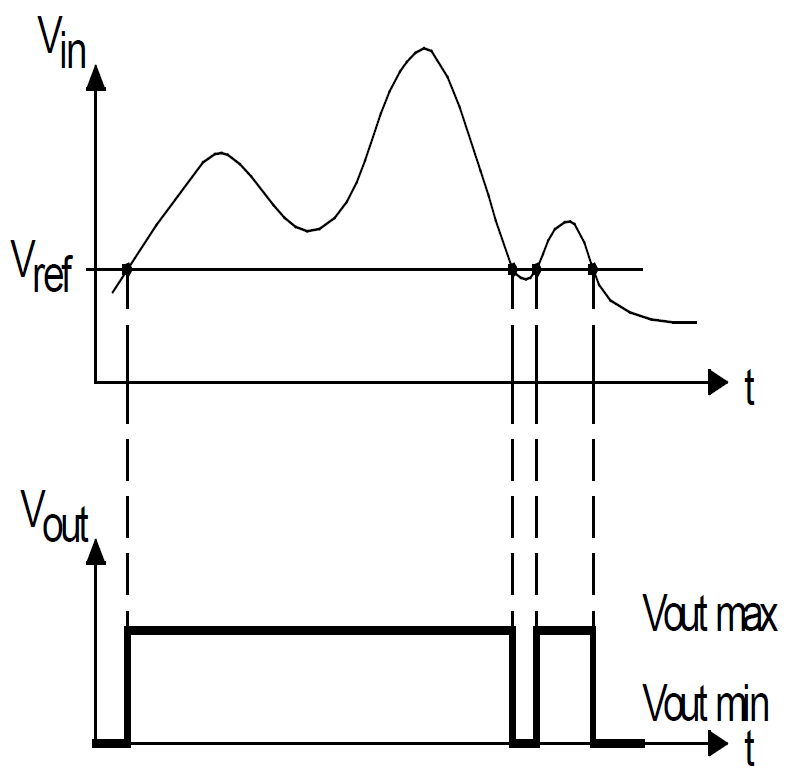
\includegraphics[width=0.75\columnwidth]{images/signalverlauf_komparator.png}
    \end{center}

    \begin{itemize}
        \item 1 Schaltschwelle
        \item Glitches möglich
    \end{itemize}
\end{minipage}
\hfill
\begin{minipage}{0.48\columnwidth}
    \begin{center}
        \myul{\textbf{Schmitt-Trigger}}
        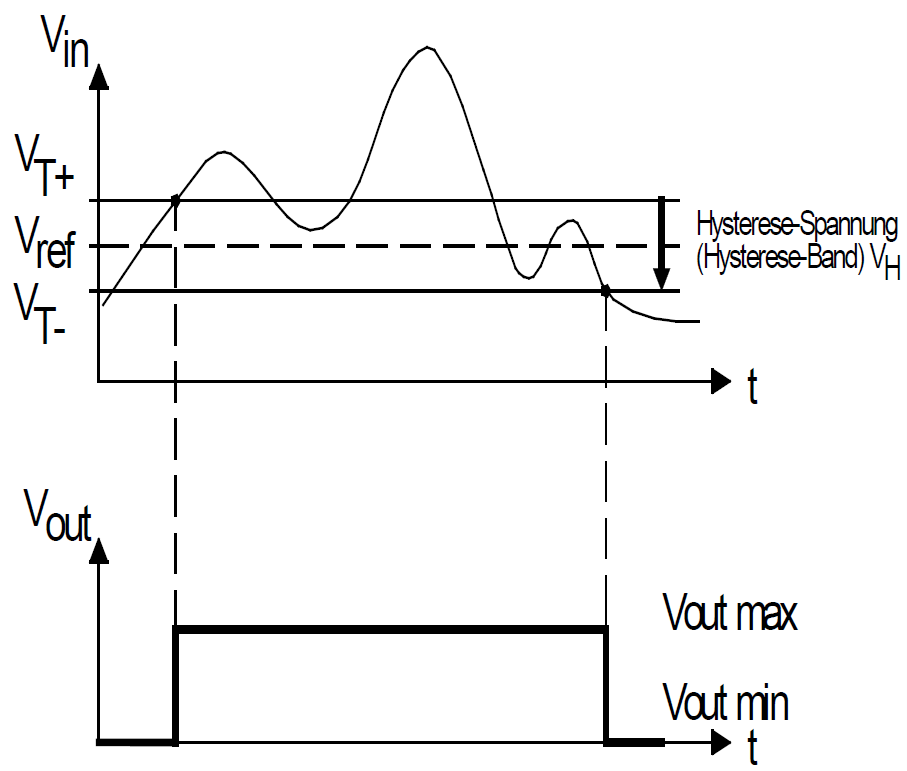
\includegraphics[width=0.8\columnwidth]{images/signalverlauf_schmitt-trigger.png}
    \end{center}

    \begin{itemize}
        \item 2 Schaltschwelle
        \item Glitches unterdrückt
        \item Hystere-Spannung $V_H$
    \end{itemize}
\end{minipage}


\subsection{Invertierender Schmitt-Trigger}

\begin{minipage}[c]{0.45\columnwidth}
    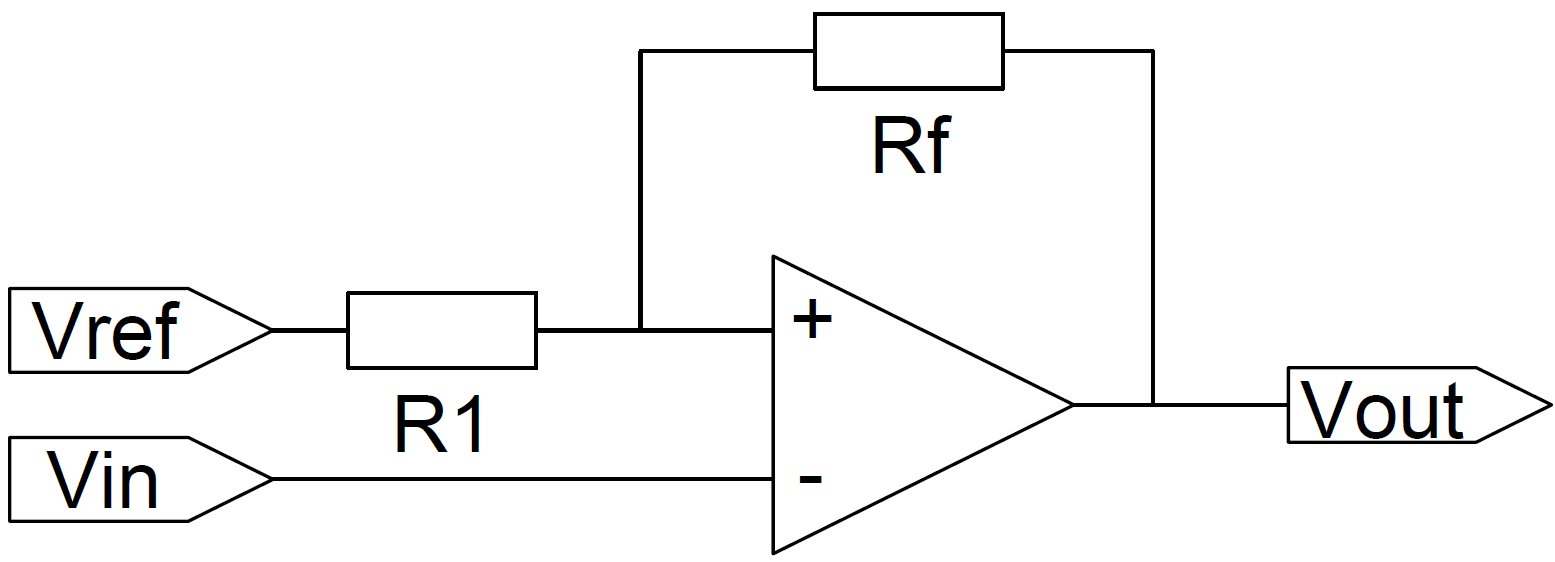
\includegraphics[width=\columnwidth]{images/invertierender_schmitt-trigger.png} 

    \vspace{0.1cm}

    Schaltet, wenn $V_{\rm in} = V_{\rm opp}$
\end{minipage}
\hfill
\begin{minipage}[c]{0.51\columnwidth}
    \begin{center}
        \myul{\textbf{Hysterese}}
        $$ \boxed{ V_H = V_{T-} - V_{T+} } $$
        $$ \boxed{ V_H = (V_{\rm out_{max}} - V_{\rm out_{min}} ) \frac{R_1}{R_1 + R_f} } $$
    \end{center}
\end{minipage}

\vspace{0.2cm}

$$ \boxed{ V_{\rm in} \text{-tief:} \quad V_{T+} = V_{\rm opp} = \frac{V_{\rm ref} \cdot R_f + V_{\rm out_{max}} \cdot R_1 }{R_1 + R_f} }  $$
$$ \boxed{ V_{\rm in} \text{-hoch:} \quad V_{T-} = V_{\rm opp} =  \frac{V_{\rm ref} \cdot R_f + V_{\rm out_{min}} \cdot R_1 }{R_1 + R_f} } $$


\subsection{Nicht-Invertierender Schmitt-Trigger}

\begin{minipage}[c]{0.45\columnwidth}
    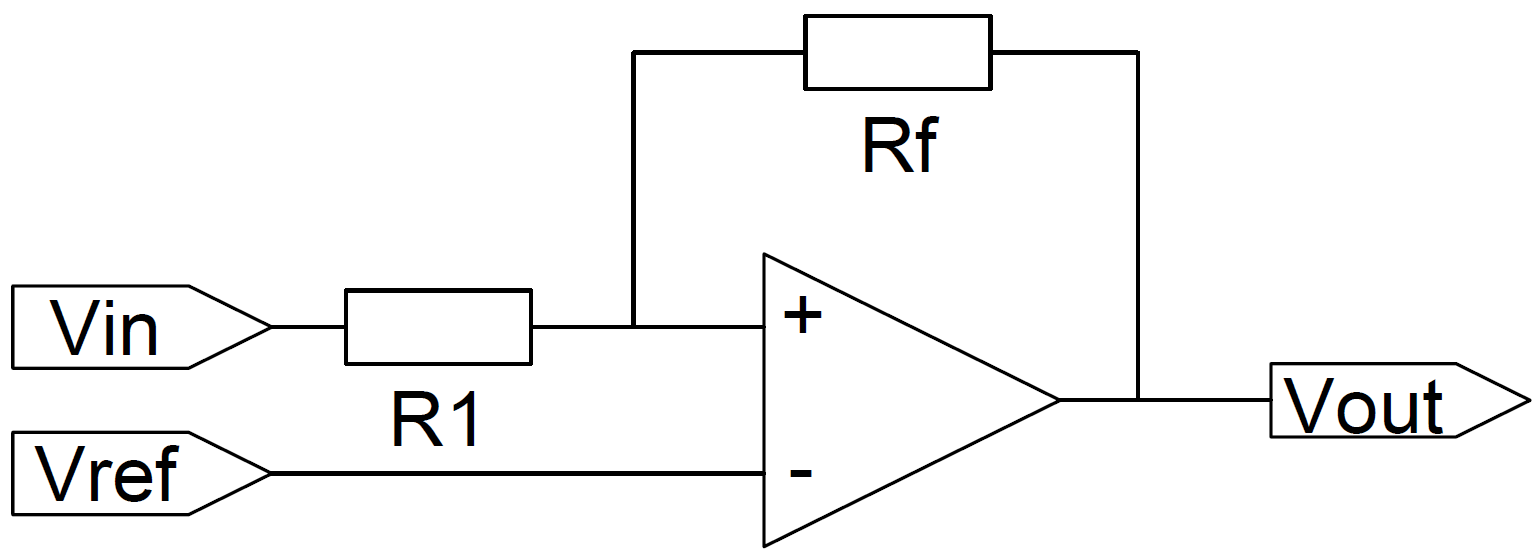
\includegraphics[width=\columnwidth]{images/nichtinvertierender_schmitt-trigger.png}

    \vspace{0.1cm}

    Schaltet, wenn $V_{\rm opp} = V_{\rm ref}$
\end{minipage}
\hfill
\begin{minipage}[c]{0.51\columnwidth}
    \begin{center}
        \myul{\textbf{Hysterese}}
        $$ \boxed{ V_H = V_{T+} - V_{T-} } $$
        $$ \boxed{ V_H = (V_{\rm out_{max}} - V_{\rm out_{min}} ) \frac{R_1}{R_f} } $$
    \end{center}
\end{minipage}


\begin{minipage}[t]{0.6\columnwidth}
    $$ \boxed{ V_{\rm in} \text{-hoch: } \quad V_{T-} = V_{\rm ref} \frac{R_1 + R_f}{R_f} - V_{\rm out_{max}} \frac{R_1}{R_f} }  $$
    $$ \boxed{ V_{\rm in} \text{-tief: } \quad V_{T+} = V_{\rm ref} \frac{R_1 + R_f}{R_f} - V_{\rm out_{min}} \frac{R_1}{R_f} } $$
\end{minipage}
\hfill
\begin{minipage}[t]{0.35\columnwidth}
    $$ \boxed{ V_{\rm opp} = \frac{  V_{\rm in} \cdot R_f + V_{\rm out} \cdot R_1}{R_1 + R_f} } $$
\end{minipage}

\vspace{0.2cm}

\textbf{Nachteil invertierender Schmitt-Trigger:} \\
'Kick-Back' auf Eingang wenn Ausgang schaltet

\vspace{0.2cm}

\textbf{Nachteil nicht-invertierender und invertierender Schmitt-Trigger:} \\
Hysterese und Schaltschwellen nicht unabhängig einstellbar


\subsection{Schmitt-Trigger mit frei wählbaren Schaltschwellen}

\begin{minipage}{0.38\columnwidth}
    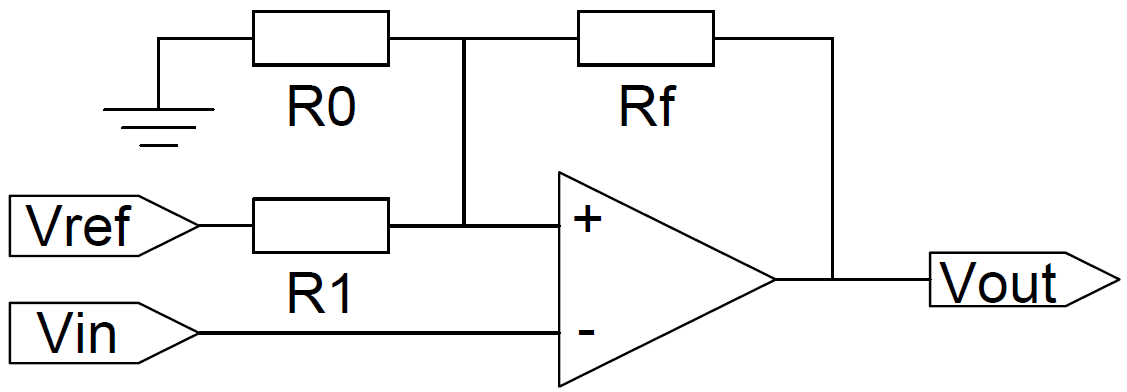
\includegraphics[width=\columnwidth]{images/inv_schmitt-trigger_schaltschwellen.png}
\end{minipage}
\hfill
\begin{minipage}{0.55\columnwidth}
    $$ \boxed{ V_{\rm opp} = V_{\rm ref} \, \frac{R_f || R_0}{R_1 + R_f || R_0} + V_{\rm out} \, \frac{R_1 || R_0}{R_1 || R_0 + R_f} } $$
\end{minipage}

\vspace{0.2cm}

2 Gleichungen, 3 Variablen ($R_0$, $R_1$, $R_f$) \\
\textrightarrow\ 1 Widerstand wird gewählt (z.B. $R_f = 100 \, \mathrm{k \Omega}$)


		\section{Digital-Analog-Wandler (DAC)}

\begin{minipage}[c]{0.42\columnwidth}
    \begin{tabular}{ll}
        $n$ & Anzahl Bits               \\
        $D$ & Digitaler Wert $D < 2^n$  \\
        $q$ & Quantisierungsschritt
  \end{tabular}
\end{minipage}
\hfill
\begin{minipage}[c]{0.54\columnwidth}
    $$ \boxed{ q = \frac{V_{\rm refp} - V_{\rm refn}}{2^n} } $$
    $$ \boxed{ V_{\rm out} =  \frac{D}{2^n} \, (V_{\rm refp} - V_{\rm refn}) + V_{\rm refn} } $$
\end{minipage}


\subsection{Parallelverfahren}

\subsubsection{Voltage Scaling - String DAC (3 Bit)}


\begin{minipage}[c]{0.15\columnwidth}
    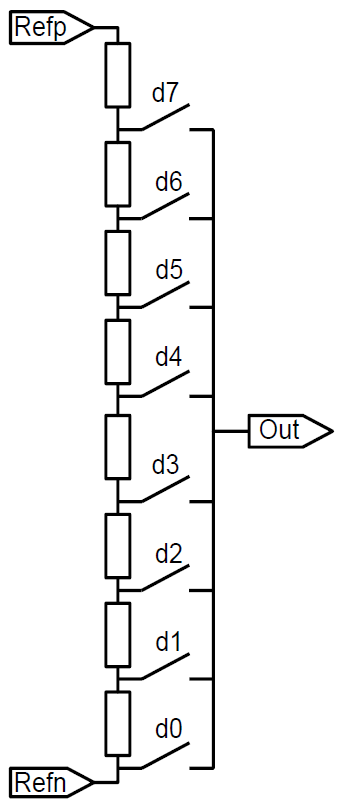
\includegraphics[height=3cm]{images/string_DAC.png}	% naja...
\end{minipage}
\hfill
\begin{minipage}[c]{0.8\columnwidth}
    Jeweils nur \textbf{ein Schalter} geschlossen

    \vspace{0.1cm}

    \begin{minipage}[c]{0.48\columnwidth}
        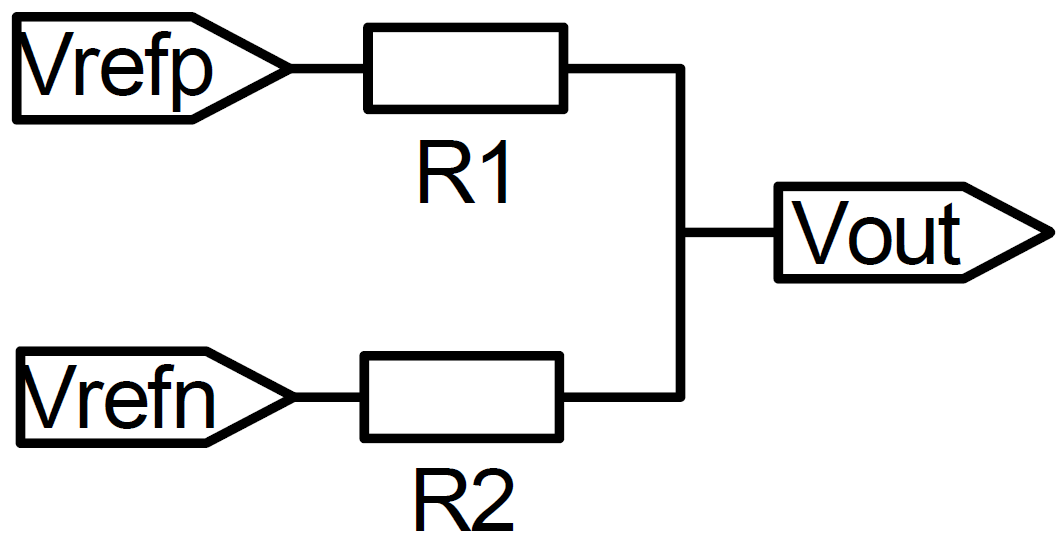
\includegraphics[width=0.95\columnwidth]{images/string_DAC_ersatzschaltung.png}
    \end{minipage}
    \hfill
    \begin{minipage}[c]{0.48\columnwidth}
        $R_1$: 1R \ldots 8R                                 \\
        $R_2$: 0R \ldots 7R                                 \\
        $V_{\rm out_{min}} = V_{\rm refn}$                  \\
        $V_{\rm out_{max}} = V_{\rm refp} - 1 \text{ LSB}$ 
    \end{minipage}

    \vspace{0.1cm}

    \begin{itemize}
        \item[+] Garantiert Stetigkeit
        \item $2^n$ Widerstände, $2^n$ Schalter \textrightarrow\ $n-\mathrm{to}-2^n$ Decoder
    \end{itemize}
\end{minipage}


\subsubsection{Voltage Scaling - String DAC (3 Bit)}

\begin{minipage}[c]{0.22\columnwidth}
    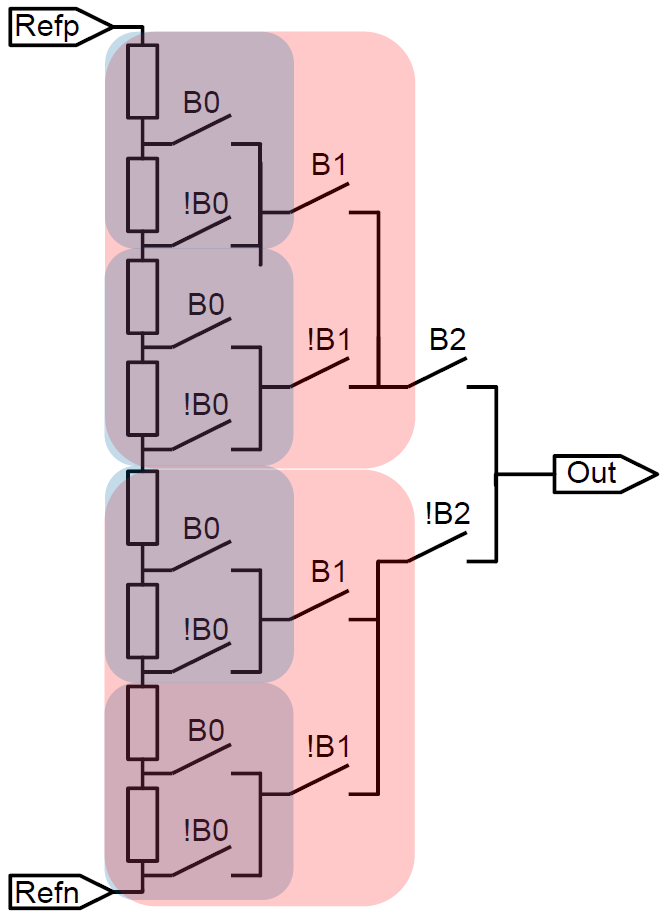
\includegraphics[width=\columnwidth]{images/string_DAC_advanced.png}
\end{minipage}
\hfill
\begin{minipage}[c]{0.76\columnwidth}
    Benötigt keinen Decoder aber zusätzliche Schalter

    \vspace{0.2cm}

    3-Bit DAC besteht aus: 

    \vspace{0.1cm}

    \begin{itemize}
        \item \cvt{4 mal 1-Bit DAC in Serie} 
        \item \crd{2 mal 2-Bit DAC in Serie}
    \end{itemize}

    \vspace{0.1cm}

    \textrightarrow\ Mit 2 mal 3-Bit DAC und Umschalter wird 4-Bit DAC gebaut
\end{minipage}


\subsubsection{Strom-DAC nach Parallelverfahren}

\begin{minipage}[c]{0.48\columnwidth}
    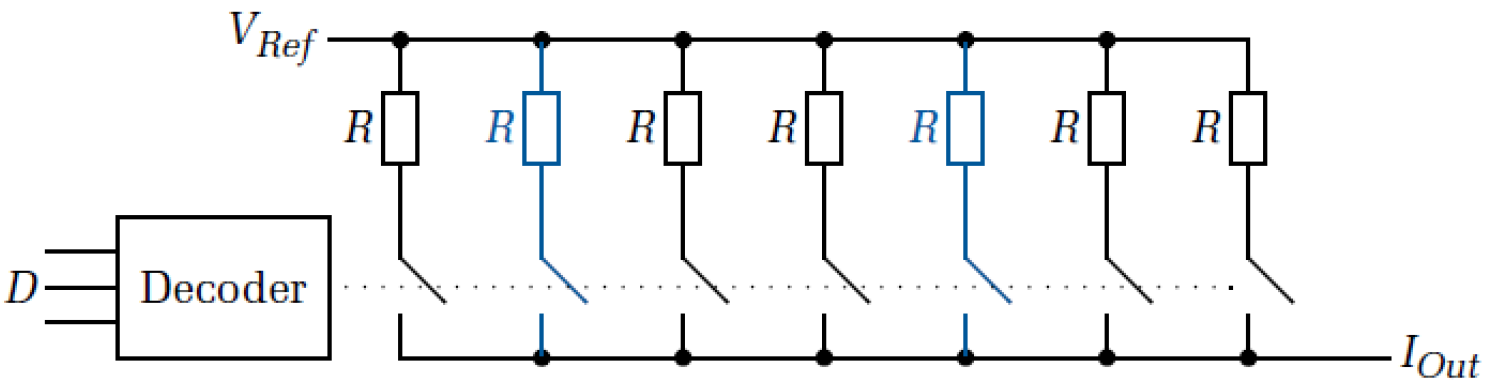
\includegraphics[width=\columnwidth]{images/strom_DAC_widerstaende.png} 
    $$ \boxed{ I_{\rm out} = D \frac{V_{\rm ref}}{R} } $$
\end{minipage}
\hfill
\begin{minipage}[c]{0.48\columnwidth}
    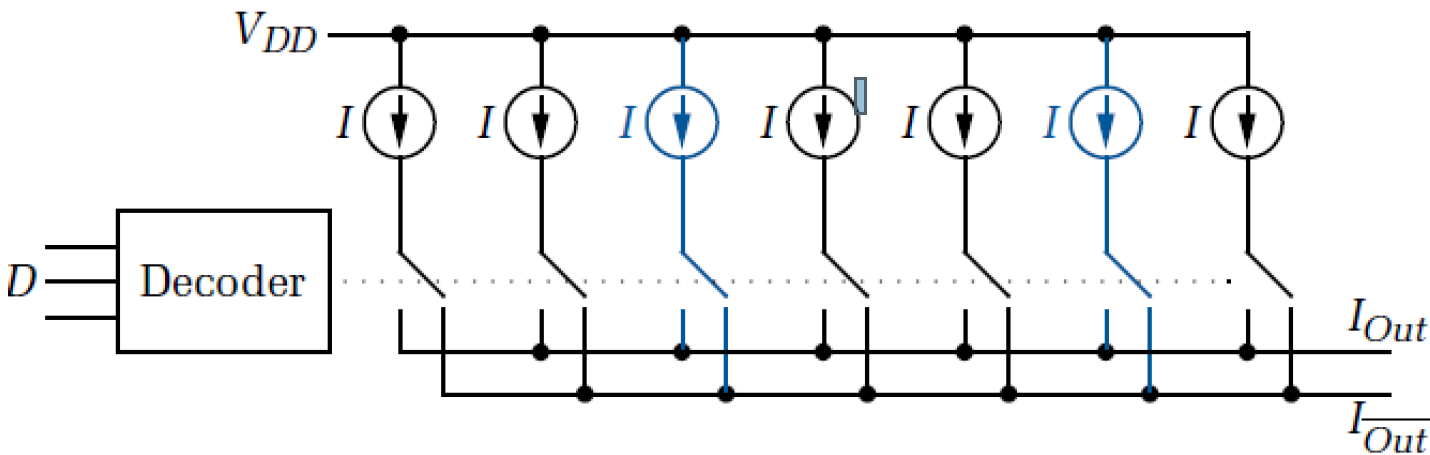
\includegraphics[width=\columnwidth]{images/strom_DAC_stromquellen.png}
    $$ \boxed{ I_{\rm out} = D \cdot I } $$
\end{minipage}

\vspace{0.2cm}

Um eine Ausgangsspannung $V_{\rm out}$ zu erhalten, wird ein OPV nachgeschaltet gemäss Kapitel \ref{R2R}

\columnbreak


\subsection{Wägeverfahren}

\subsubsection{Wägeverfahren -- resistiv}

\begin{minipage}[c]{0.4\columnwidth}
    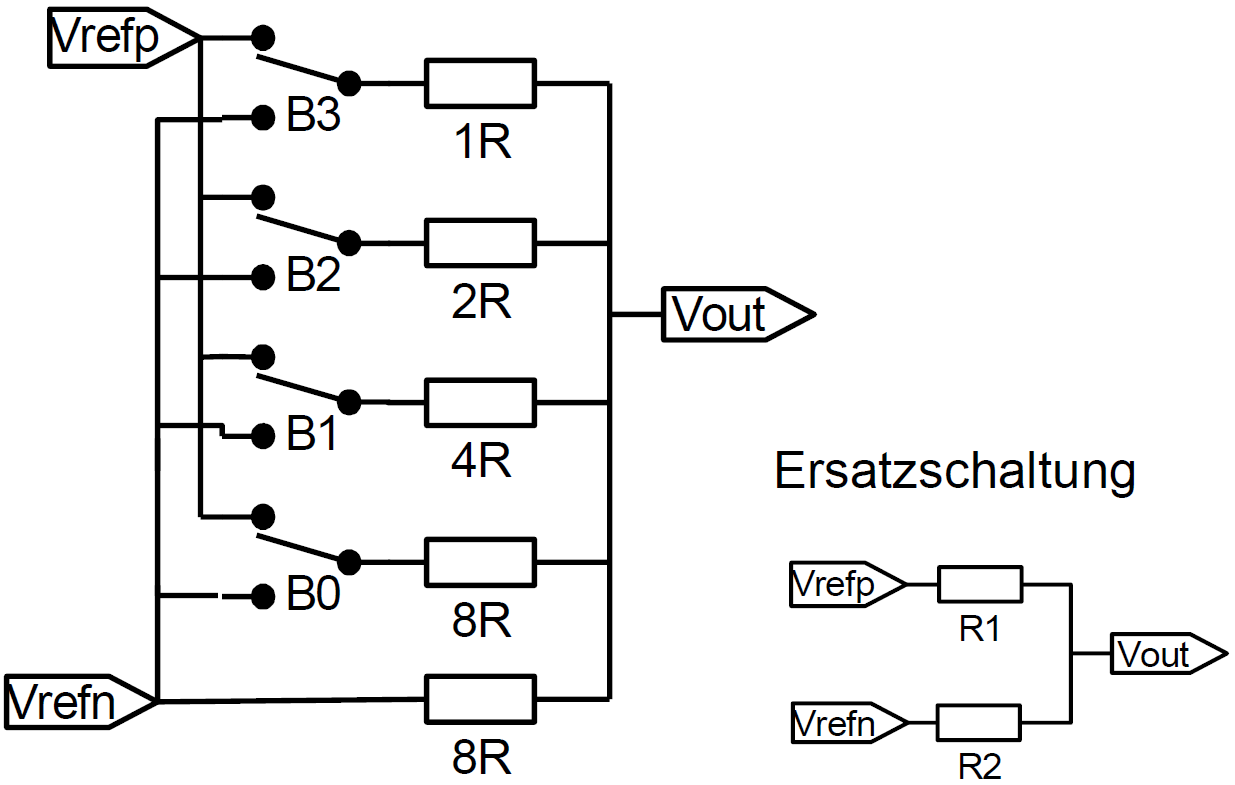
\includegraphics[width=\columnwidth]{images/waegeverfahren.png}
\end{minipage}
\hfill
\begin{minipage}[c]{0.53\columnwidth}
    \begin{itemize}
        \item[+] $N$ Widerstände, $N$ Schalter 
        \item[-] Nicht garantiert stetig
        \item[-] Grosser Wertebereich der Widerstände nötig 
    \end{itemize}

    $$ \textbf{Leitwerte!} \qquad \bm{G_0 = \frac{1}{8R} } $$
\end{minipage}

$$ \boxed{ V_{\rm out} = \frac{B_0 \cdot 2^0 \cdot G_0 + B_1 \cdot 2^1 \cdot G_0 + B_2 \cdot 2^2 \cdot G_0+ B_3 \cdot 2^3 \cdot G_0}{2^4 \cdot G_0} (V_{\rm refp}- V_{\rm refn}) + V_{\rm refn} } $$


\subsubsection{Kapazitiver DAC ohne Ausgangsbuffer (4 Bit)}

\begin{center}
    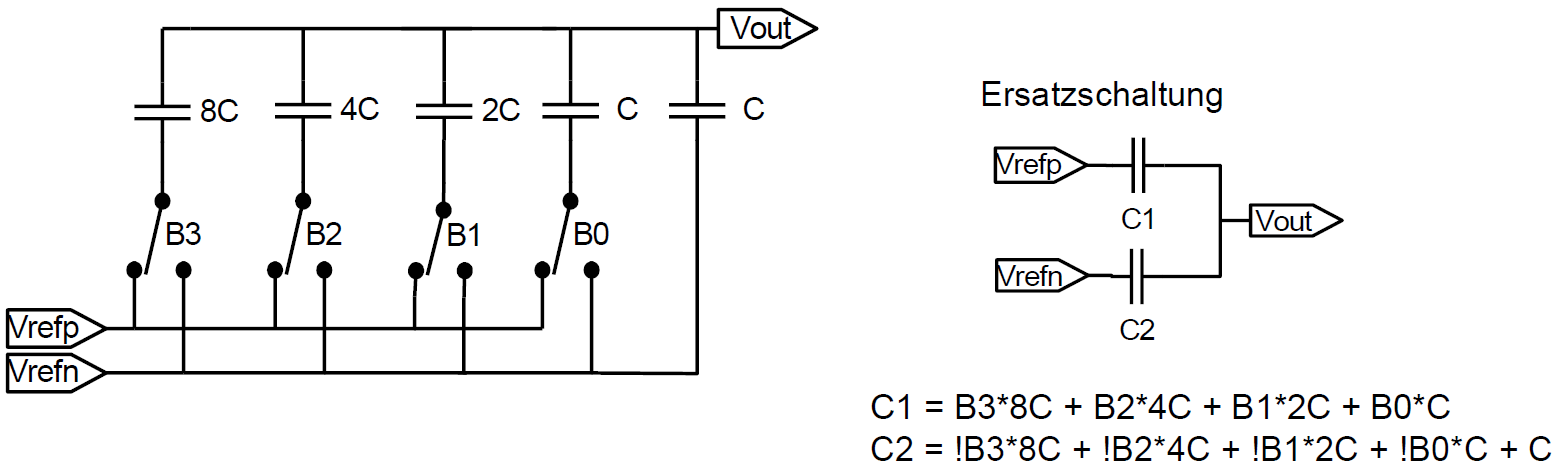
\includegraphics[width=0.85\columnwidth]{images/kapazitiver_DAC_2.png}
\end{center}

Wenn Kapazitäten entladen sind, bevor geschaltet wird: 
$$ \boxed{ V_{\rm out} = \frac{C_1}{C_1 + C_2} (V_{\rm refp} - V_{\rm refn}) + V_{\rm refn}  \quad  \text{mit } C_1 + C_2 = 2^n \cdot C } $$

\textbf{Problem:} Lastkapazitäten an $V_{\rm out}$ \textrightarrow\ Schaltung so schlecht brauchbar  


\subsubsection{Kapazitiver DAC mit Ausgangsbuffer}

\begin{minipage}[c]{0.4\columnwidth}
    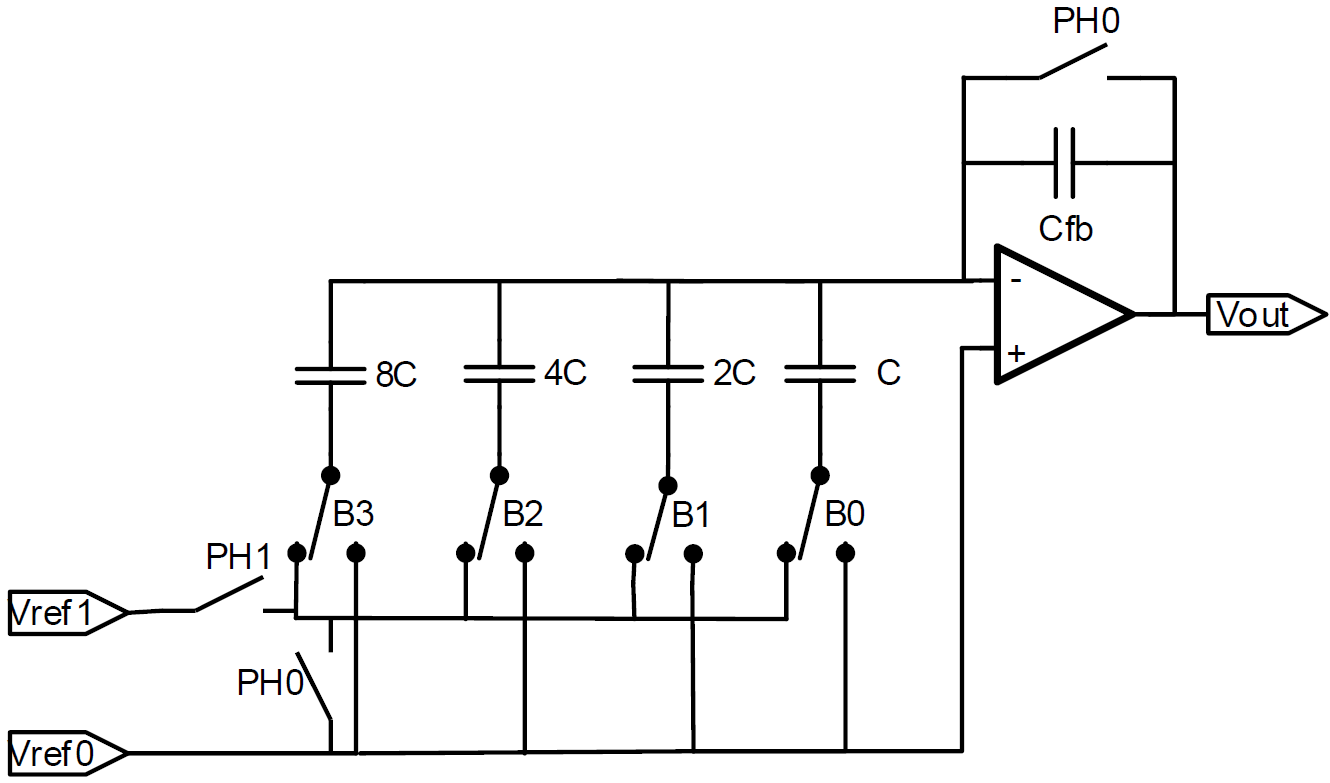
\includegraphics[width=\columnwidth]{images/kapazitiver_DAC_ausgangsbuffer.png}
\end{minipage}
\hfill
\begin{minipage}[c]{0.53\columnwidth}
    \raggedright
    Immer nur ein Schalter geschlossen! \\
    2 Phasen: PH0 und PH1 

    \vspace{0.2cm}
    PH0: $V_{\rm out} = V_{\rm ref0}$ \\
    PH1: Ausgang gültig (nach Einschwingen)

    $$ \boxed{ V_{\rm out} = -(V_{\rm ref1} - V_{\rm ref0}) \cdot \Bigg( \frac{n \cdot C}{C_{fb}}  \Bigg) + V_{\rm ref0} } $$
\end{minipage}

\vspace{0.2cm}

\textbf{Nachteil:} Sample-Hold nötig für Ausgangsspannung in Phase PH0 (wenn Schalterstellung gewechselt wird)


\subsubsection{Wägeverfahren mit Widerständen und Ausgangsverstärker}

\begin{minipage}[c]{0.45\columnwidth}
    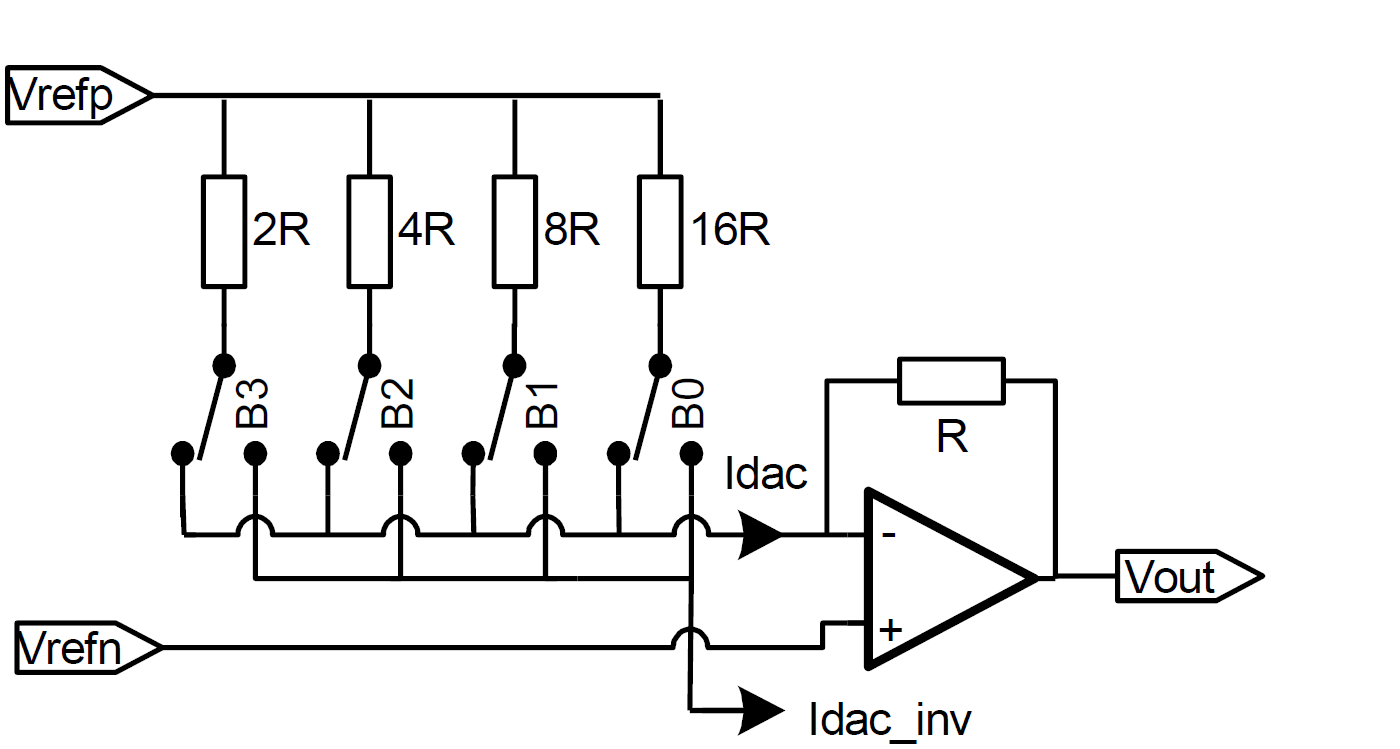
\includegraphics[width=\columnwidth]{images/DAC_ausgangsverstaerker.png}
\end{minipage}
\hfill
\begin{minipage}[c]{0.53\columnwidth}
    $$ \boxed{ I_{\rm dac_{max}} = \frac{V_{\rm refp} - V_{\rm refn}}{R} \frac{2^n -1}{2^n} } $$
    $$ \boxed{ I_{\rm dac} = \frac{V_{\rm refp} - V_{\rm refn}}{R} \frac{D}{2^n}  } $$
    $$ \boxed{ V_{\rm out} = V_{\rm refn} - R \cdot I_{\rm dac} } $$

    \vspace{0.2cm}
    \begin{itemize}
        \item[+] differentiell ($I_{\rm dac_{inv}}$)
        \item[-] Ausgang darf belastet werden
    \end{itemize}
\end{minipage}


\subsubsection{DAC mit R2R-Netzwerk}
\label{R2R}

\begin{minipage}[c]{0.4\columnwidth}
    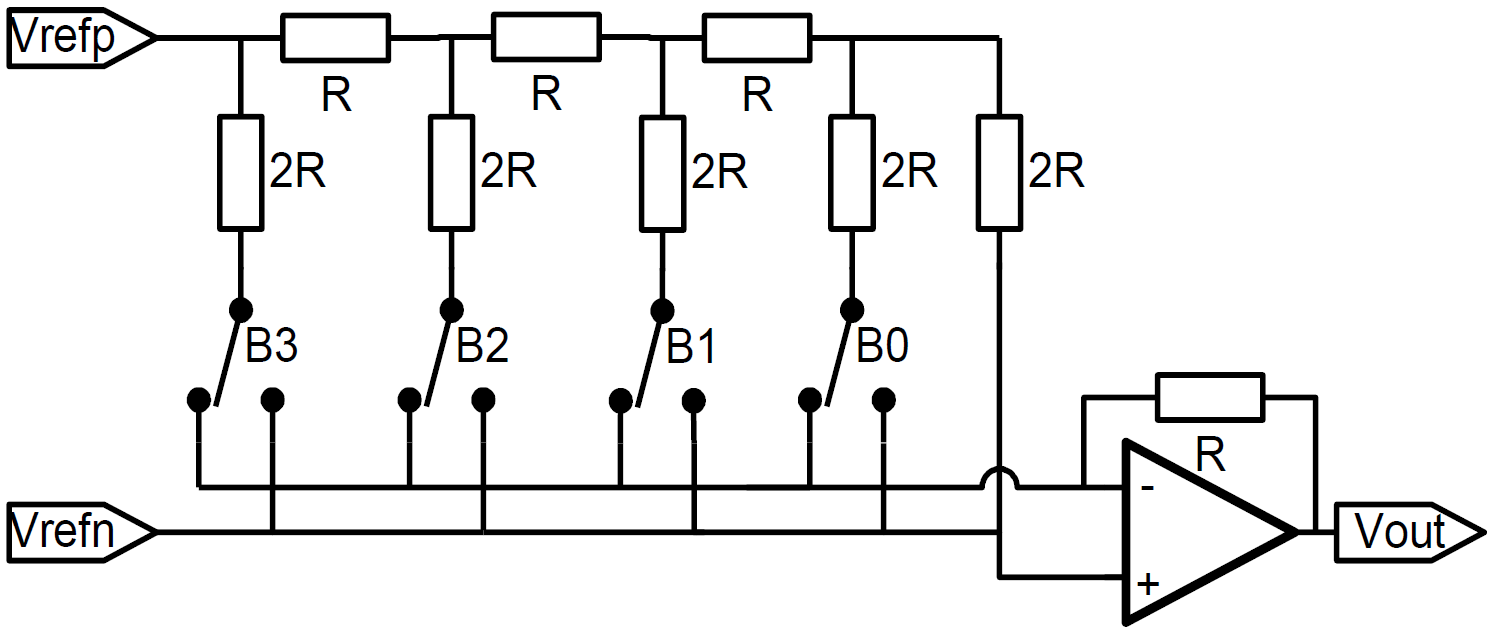
\includegraphics[width=\columnwidth]{images/R2R_netzwerk}
\end{minipage}
\hfill
\begin{minipage}[c]{0.56\columnwidth}
    Für Ersatzwiderstand \textbf{von rechts} her 'schauen'

    \vspace{0.2cm}
    
    \begin{itemize}
        \item[+] Nur 2 Widerstandswerte: R, 2R
        \item[+] Gute Alternative zu gewichteten R's bzw. C's
        \item[+] Stromgewichtung über Spannungsteiler von $V_{\rm refp}$ zu $V_{\rm refn}$
    \end{itemize}
\end{minipage}

\vspace{0.2cm}
Variiert $V_{\rm refp}$, dann variiert auch $V_{\rm out}$

\textbf{Jeder geschlossene Schalter trägt gewichtet zur Ausgangsspannung bei! \\
Achtung: Invertierung!}

$$ \boxed{V_{\rm out} = V_{\rm refn} - (V_{\rm refp} - V_{\rm refn}) \cdot \frac{D}{2^n}}  $$


\cbl{\myul{\textbf{Beispiel:}}

\renewcommand{\arraystretch}{1.8}
\begin{tabular}{lll}
    $B_3 \text{ geschlossen: } V_{\rm out} = V_{\rm refn} - \frac{\Delta V_{\rm ref}}{2}$    & & 
    $B_2 \text{ geschlossen: } V_{\rm out} = V_{\rm refn} - \frac{\Delta V_{\rm ref}}{4}$    \\
    $B_1 \text{ geschlossen: } V_{\rm out} = V_{\rm refn} - \frac{\Delta V_{\rm ref}}{8}$    & & 
    $B_0 \text{ geschlossen: } V_{\rm out} = V_{\rm refn} - \frac{\Delta V_{\rm ref}}{16}$
\end{tabular}
}
\renewcommand{\arraystretch}{1}


\subsection{Einschub: Kapazitiver Spannungsteiler}

\begin{minipage}[c]{0.4\columnwidth}
    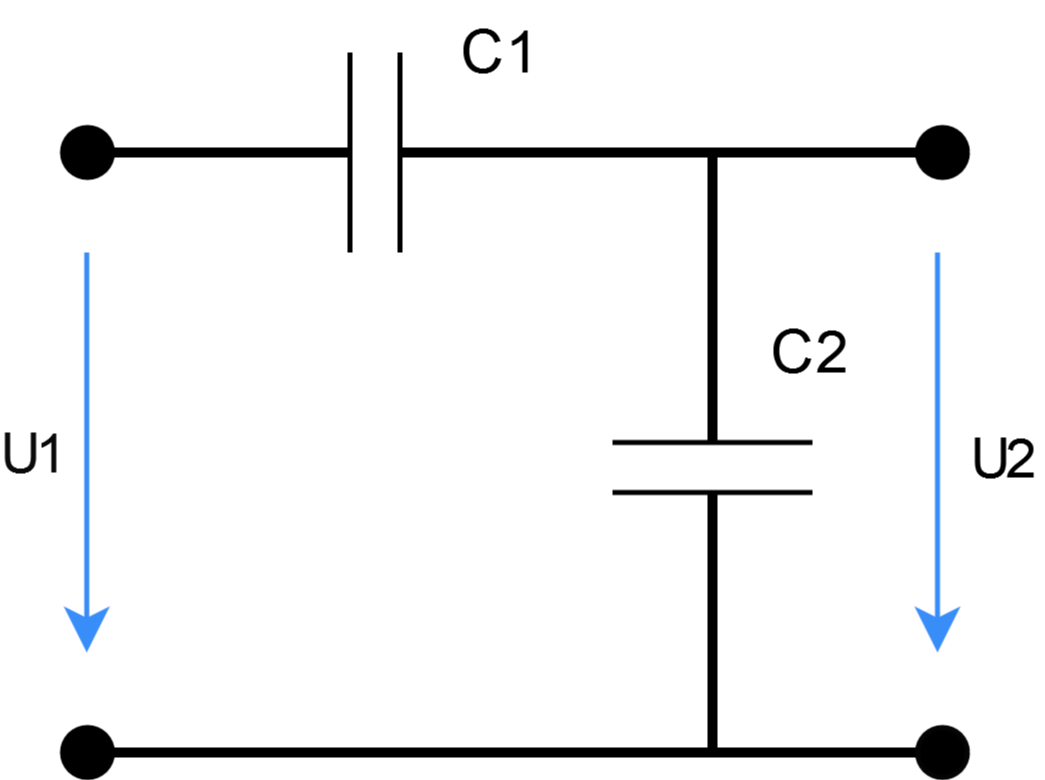
\includegraphics[width=0.7\columnwidth]{images/CapSpannungsteiler.png} 
\end{minipage}
\hfill
\begin{minipage}[c]{0.58\columnwidth}
    $$ \boxed{ U_2 = U_1 \cdot \frac{X_2}{X_1 + X_2} = U_1 \cdot \frac{C_1}{C_1 + C_2} } $$
\end{minipage}


\subsection{Zählverfahren (PWM)}

\subsubsection{PWM: Pulse Width Modulation}

\begin{minipage}[c]{0.45\columnwidth}
    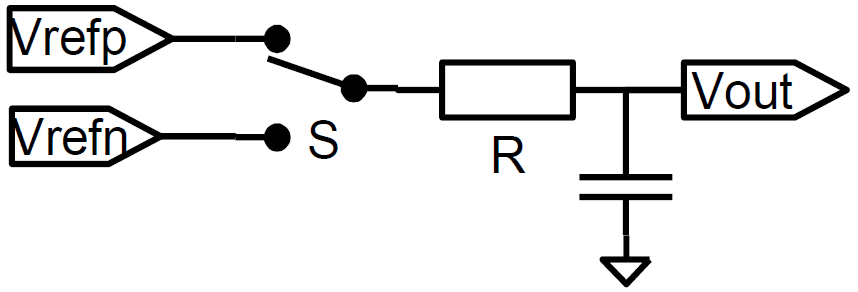
\includegraphics[width=\columnwidth]{images/PWM_DAC}
\end{minipage}
\hfill
\begin{minipage}[c]{0.52\columnwidth}
    \raggedright
    $S$ schaltet zwischen $V_{\rm refp}$ und $V_{\rm refn}$ (\textrightarrow\ PWM) \\
    (\textrightarrow\ meistens $V_{\rm ref}$ und $GND$ )

    \vspace{0.2cm}

    \textbf{RC glättet und erzeugt 'DC'}
\end{minipage}

\vspace{0.2cm}

\begin{minipage}[c]{0.48\columnwidth}
    \begin{itemize}
        \item[+] Sehr einfache Schaltung
        \item[+] Ermöglicht hohe Auflösung 
        \item[+] Funktioniert onchip digital (z.B. FPGA, $\mu$C) \textrightarrow\ analoge Schaltung extern
    \end{itemize}
\end{minipage}
\hfill
\begin{minipage}[c]{0.48\columnwidth}
    \raggedright
    \begin{itemize}
        \item[-] Sehr langsam
        \item[-] Benötigt grosses $\tau$ für kleine Spannungsrippel (oder Tiefpass höherer Ordnung)
    \end{itemize}
\end{minipage}

\vspace{0.2cm}

\myul{\textbf{PWM-Ansteuerung für Schalter $\bm{S}$}}

\vspace{0.1cm}

\begin{minipage}[c]{0.4\columnwidth}
    $$ \boxed{ \overline{V_{\rm out}} = V_{\rm ref} \cdot \frac{n}{N} }  $$
\end{minipage}
\hfill
\begin{minipage}[c]{0.58\columnwidth}
    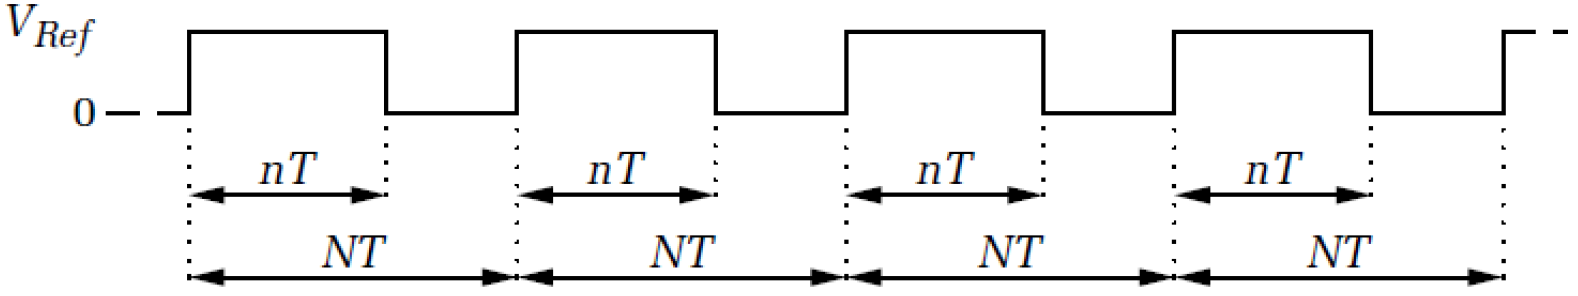
\includegraphics[width=\columnwidth]{images/PWM_ansteuerung_2.png} 
\end{minipage}


\subsection{Kaskadierte Wandler und Mischformen}

\subsubsection{Kaskadierte DACs}

\begin{minipage}[c]{0.6\columnwidth}
    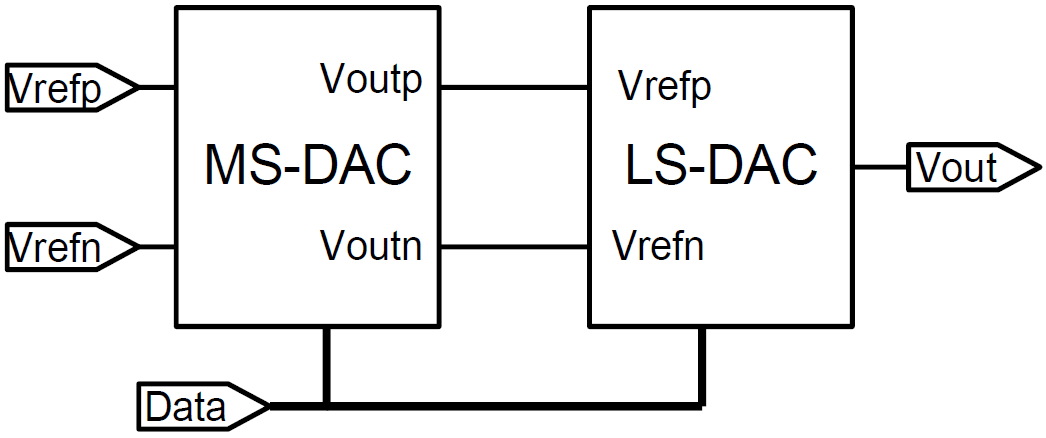
\includegraphics[width=0.75\columnwidth]{images/kaskadierte_DAC_1.png}
\end{minipage}
\hfill
\begin{minipage}[c]{0.38\columnwidth}
    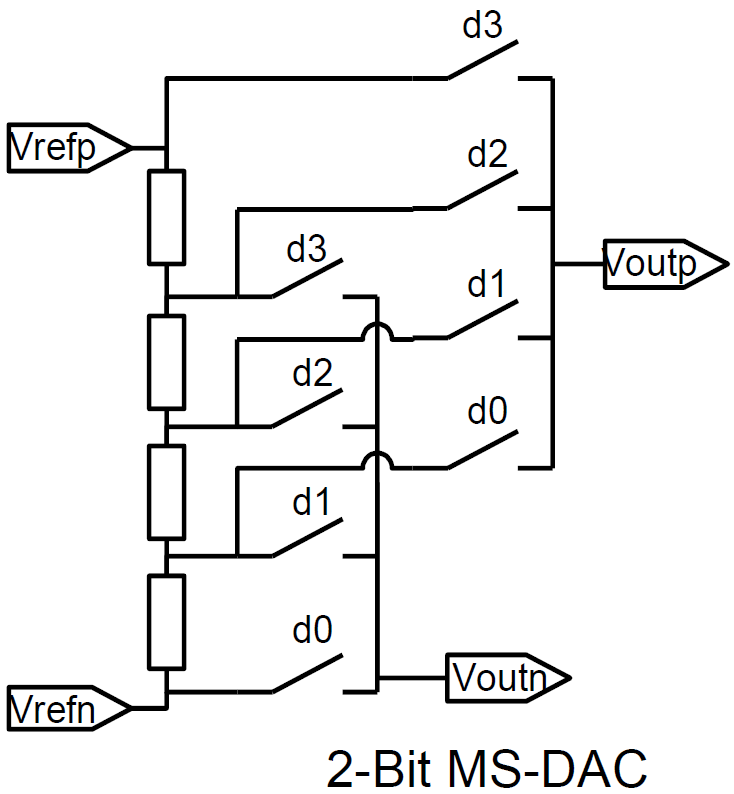
\includegraphics[width=0.7\columnwidth]{images/kaskadierte_DAC_2.png}
\end{minipage}

\vspace{0.2cm}

\begin{itemize}
    \item MS-DAC: 2 Ausgangsspannungen (über / unter gewünschtem $V_{\rm out}$)
    \item LS-DAC: folglich kleinere Eingangsspannungsdifferenz \\
        \textrightarrow\ Kleinerer Quantisierungsschritt $q$ \\
        \textrightarrow\ Höhere absolute Spannungsauflösung
\end{itemize}


\subsubsection{Segmentierter String DAC}

\begin{minipage}[c]{0.3\columnwidth}
    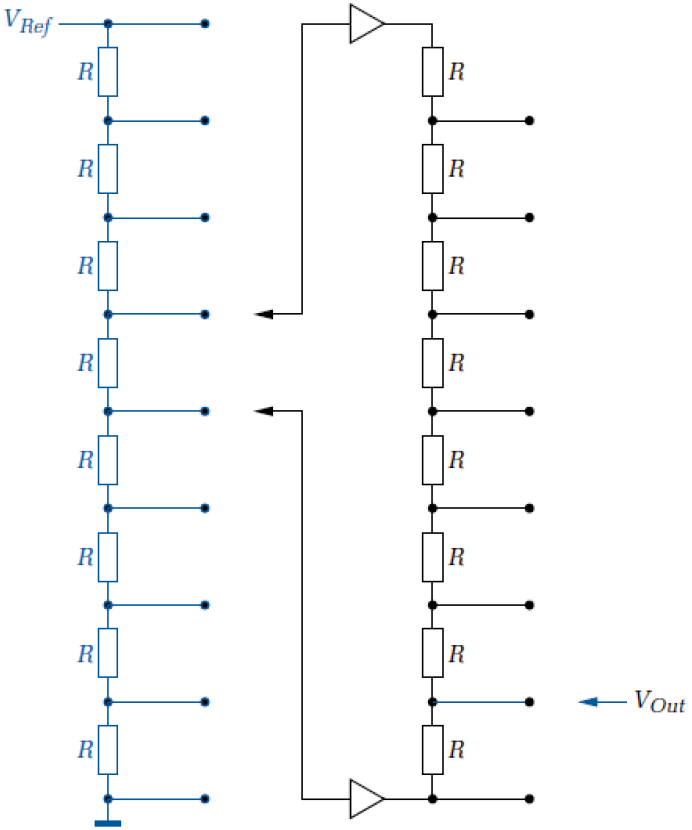
\includegraphics[width=\columnwidth]{images/segmented_string.png} 
\end{minipage}
\hfill
\begin{minipage}[c]{0.68\columnwidth}
    \begin{itemize}
        \item 2 'Strings' mit tiefer Auflösung ergeben doppelte\\
            Auflösung \textrightarrow\ $2 \cdot 8$R \textrightarrow\ $2 \cdot 3$ Bit
        
        \vspace{0.2cm}

        \item[+] Viel weniger Elemente
        \item[-] Benötigt 2 Buffer (damit keine Belastung des linkes 'Strings')
        \item[-] Buffer müsste offset-frei sein
    \end{itemize}

    \vspace{0.2cm}

    Alternative: Viel grössere R in rechtem 'String' \\
    \textrightarrow\ kleine Belastung links
\end{minipage}


\subsection{Zusammenfassung DACs}

    \begin{tabular}{ll}
    Parllelverfahren    & ... garantiert monotone Wandler           \\
    Wägeverfahren       & ... Anzahl Elemente nicht allzu hoch      \\
    Zählverfahren       & ... Wenn Zeit untergrodnete Rolle spielt
\end{tabular}

\vspace{0.2cm}

\textrightarrow\ \textbf{Oft werden Parallel- und Wägeverfahren kombiniert!}

\vspace{0.1cm}

Schnelle DACs haben oft einen Stromausgang und benötigen daher einen Ausgangsverstärker
\textrightarrow\ Ströme können schneller geschaltet werden als Spannungen!

\vspace{0.2cm}

Es gilt: Für optimale Resultate müssen \textbf{Kompromisse} eingegangen werden! 

		\section{Analog-Digital-Wandler (ADC)}

\begin{minipage}[c]{0.48\columnwidth}
    \begin{tabular}{ll}
        $n$         & Anzahl Bits                       \\
        $D$         & Digitaler Wert \quad $D < 2^n$    \\
        $q$         & Quantisierungsschritt             \\
        $B_0$       & Bitwert 0 (LSB)                   \\
        $B_{n-1}$   & Bitwert $n-1$ (MSB)
    \end{tabular}
\end{minipage}
\hfill
\begin{minipage}[c]{0.48\columnwidth}
    $$ \boxed{ q = \frac{V_{\rm refp} - V_{\rm refn}}{2^n} } $$
    $$ \boxed{ D = \frac{V_{\rm in} - V_{\rm refn}}{V_{\rm refp} - V_{\rm refn}} \, 2^n } $$
\end{minipage}


\subsection{Einführung}

\begin{itemize}
    \item Ein AD-Wandler ordnet einer analogen Spannung einen digitalen Wert zu
    \item Der einfachste AD-Wandler ist ein Komparator (1 Bit)
    \item \textbf{Absoluter Fehler} $E_q < \pm \frac{1}{2}$ LSB 
\end{itemize}


\subsubsection{Settling Time}

\begin{minipage}[c]{0.35\columnwidth}
    $$ \boxed{ N_{TC} = \ln(2^N)} $$
\end{minipage}
\hfill
\begin{minipage}[c]{0.62\columnwidth}
    \begin{tabular}{ll}
        $N_{TC}$    & \# $T$ für $N$ Bits Settling      \\
        $T$         & Zeitkonstante $T = RC$            \\
        $N$         & \# Bits Auflösung (Genauigkeit)
    \end{tabular}
\end{minipage}

\columnbreak

\subsubsection{Sample and Hold}

Vor einer Wandlung muss Spannung gespeichert werden (meistens)

\begin{center}
    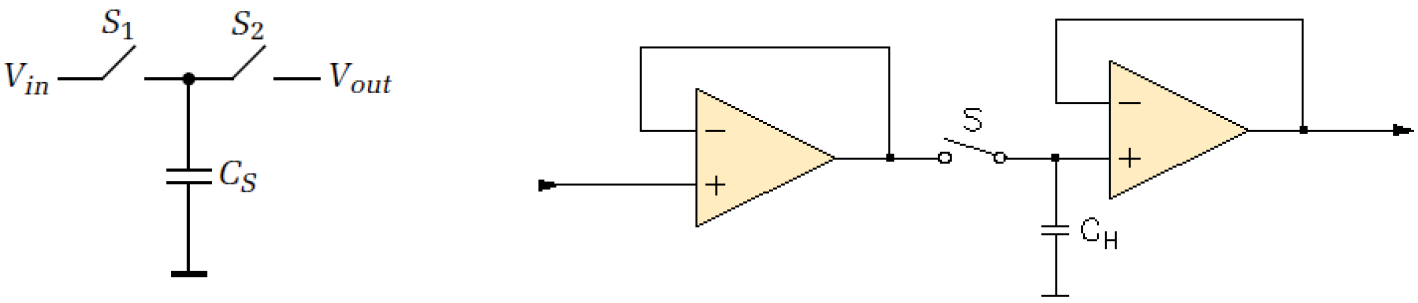
\includegraphics[width=0.8\columnwidth]{images/sample_hold.png}
\end{center}

\begin{tabular}{ll}
    links: & Belastung von Quelle und Senke \textrightarrow\ unbrauchbar! \\
    rechts & Ohne Belastung von Quelle und Senke (Buffer)  
\end{tabular}


\subsection{Parallelverfahren (Flash-Wandler)}

\subsubsection{3-Bit ADC nach Parallel-Verfahren (Flash-Wandler)}

\begin{minipage}[c]{0.38\columnwidth}
    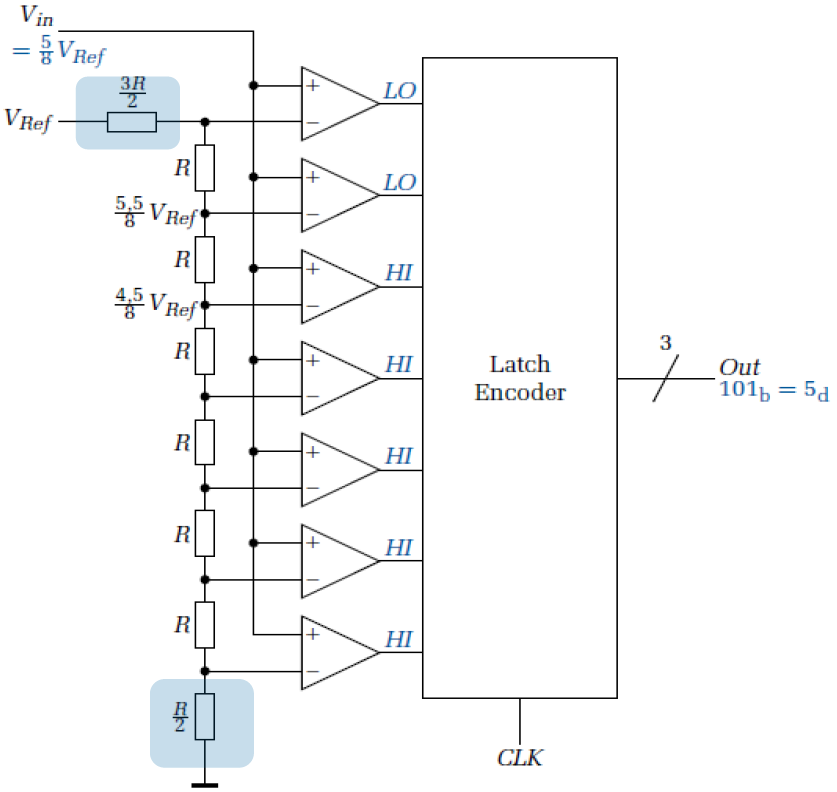
\includegraphics[width=\columnwidth]{images/ADC_parallelverfahren.png}
\end{minipage}
\hfill
\begin{minipage}[c]{0.6\columnwidth}
    \begin{itemize}
        \item[+] ADC ist \textbf{sehr schnell}
        \item[+] Nur 1 Takt
        \item[-] $2^n$ Widerstände
        \item[-] $2^n -1$ Komparatoren
    \end{itemize}
    
    \vspace{0.2cm}

    'Runden' ist möglich mit unterschiedlichen Widerständen ganz unten und ganz oben \cbl{(blau hinterlegt)} \\
    \cbl{ \textrightarrow\ 'Sprung' ist hier bei $\frac{q}{2}$ statt bei $q$}
\end{minipage}


\subsubsection{Pipeline- (Kaskaden-, Subranging-) ADC}

Kaskadierung von \textbf{Flash-ADCs}
\vspace{0.2cm} 

\begin{minipage}[c]{0.46\columnwidth}
    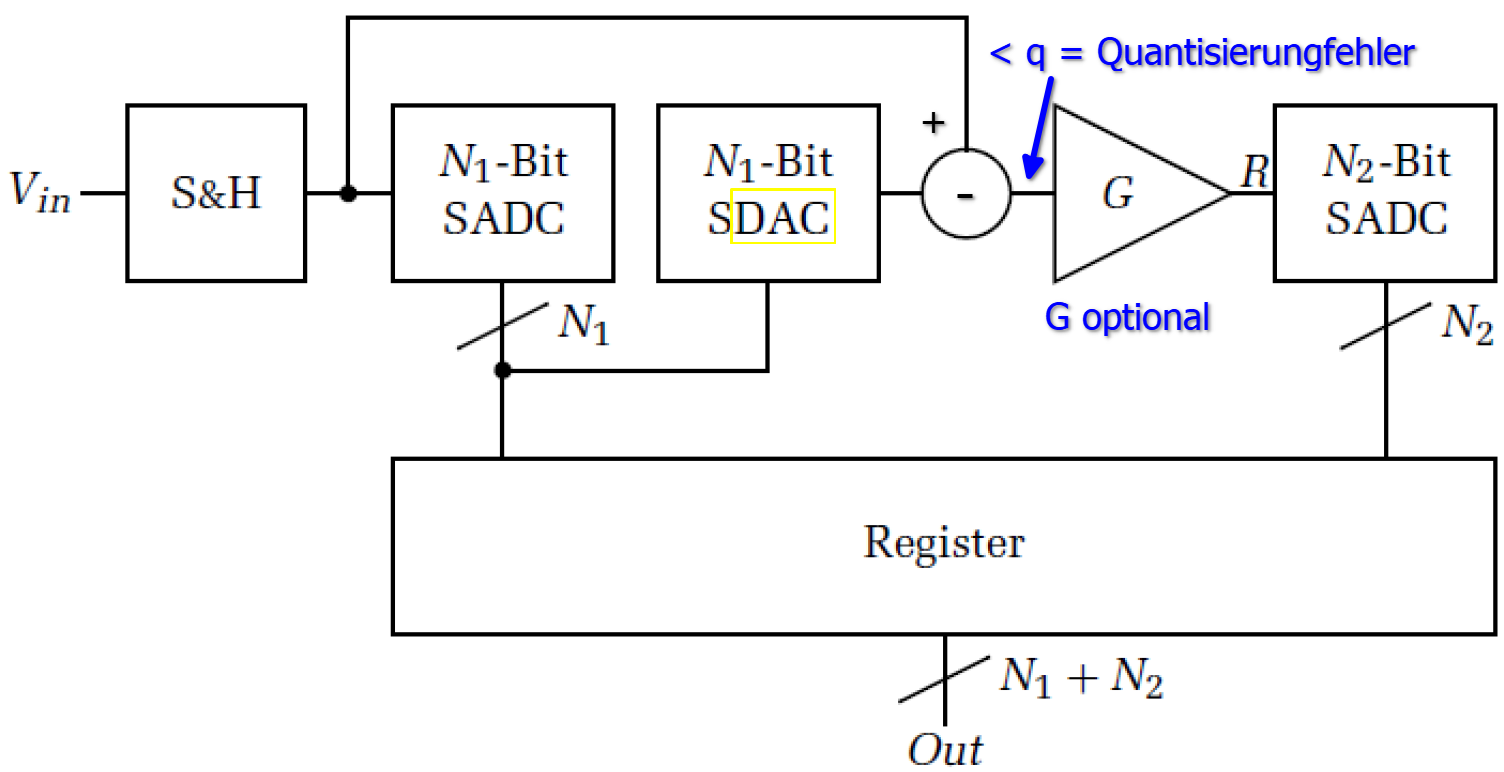
\includegraphics[width=\columnwidth]{images/pipeline_ADC.png}
\end{minipage}
\hfill
\begin{minipage}[c]{0.5\columnwidth}
    Zweistufig:

    \vspace{0.1cm}

    \begin{enumerate}
        \item ADC mit $N_1$ Bits
        \item ADC mit $N_2$ Bits
    \end{enumerate}

    \vspace{0.2cm}

    \begin{itemize}
        \item[+] Nur $2^{N_1} + 2^{N_2}$ Komparatoren
        \item[-] Braucht zusätzlichen DAC mit $N_1$ Bits
        \item[-] Braucht ev. Verstärker mit Gain $G$
    \end{itemize}
\end{minipage}

\vspace{0.2cm}

\myul{\textbf{Ablaufsteuerung Pipeline-ADC}}

\vspace{0.1cm}

\begin{minipage}[c]{0.33\columnwidth}
    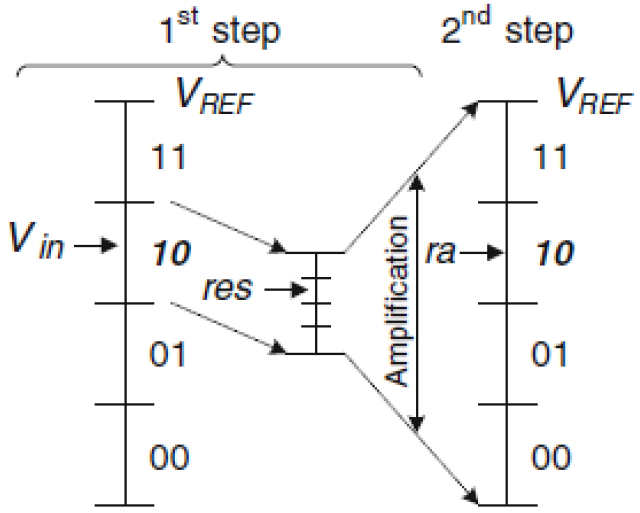
\includegraphics[width=\columnwidth]{images/ablauf_pipeline_ADC_2.png} 
\end{minipage}
\hfill
\begin{minipage}[c]{0.63\columnwidth}
    \begin{itemize}
        \item Spannungswert der digitalierten Spannung wird von $V_{\rm in}$ abgezogen
        \item Restspannung ($ < q$) wird mit $2^{N_1}$ multipliziert und digitalisiert mit $N_2$ Bits \\
            (bei gleicher Referenzspannung von 2. ADC)
    \end{itemize}
\end{minipage}


\subsubsection{Mehrstufiger Pipeline-Wandler}

\begin{center}
    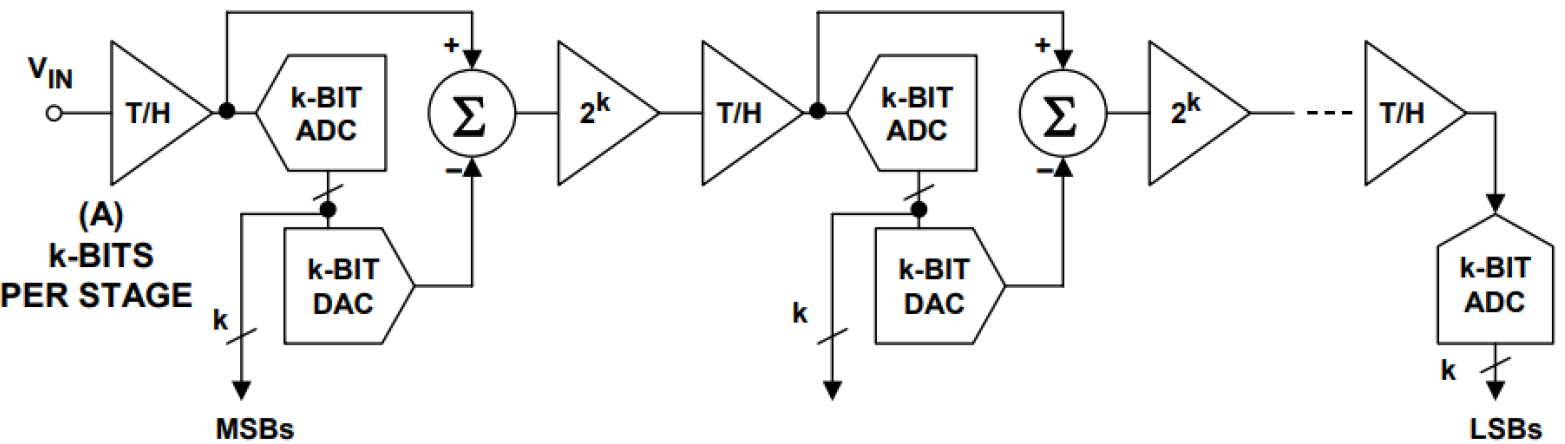
\includegraphics[width=0.8\columnwidth]{images/mehrstufiger_pipeline_wandler.png}
\end{center}


\begin{minipage}[c]{0.48\columnwidth}
    \begin{itemize}
        \item Flash-ADC mit $k \geq 1$ DAC mit $k$ Bits
        \item Multiplikation mit $2^k$ (gleiche Referenz für jede Stufe)
    \end{itemize}
\end{minipage}
\hfill
\begin{minipage}[c]{0.48\columnwidth}
    \begin{itemize}
        \item \textbf{Latenz bei $\bm{n}$ Stufen} \textrightarrow\ $n$ Zyklen
        \item Update-Frequenz $n$-mal grösser \\
            \textrightarrow\ In jedem Zyklus ein neuer Wert
    \end{itemize}
\end{minipage}

\vspace{0.2cm}

\textbf{Statt Multiplikation mit $\bm{2^k}$ kann auch die Referenzspannung der folgenden Stufe um $\bm{2^k}$ verkleinert werden!}


\subsubsection{Iterative ADC}

\begin{minipage}[c]{0.4\columnwidth}
    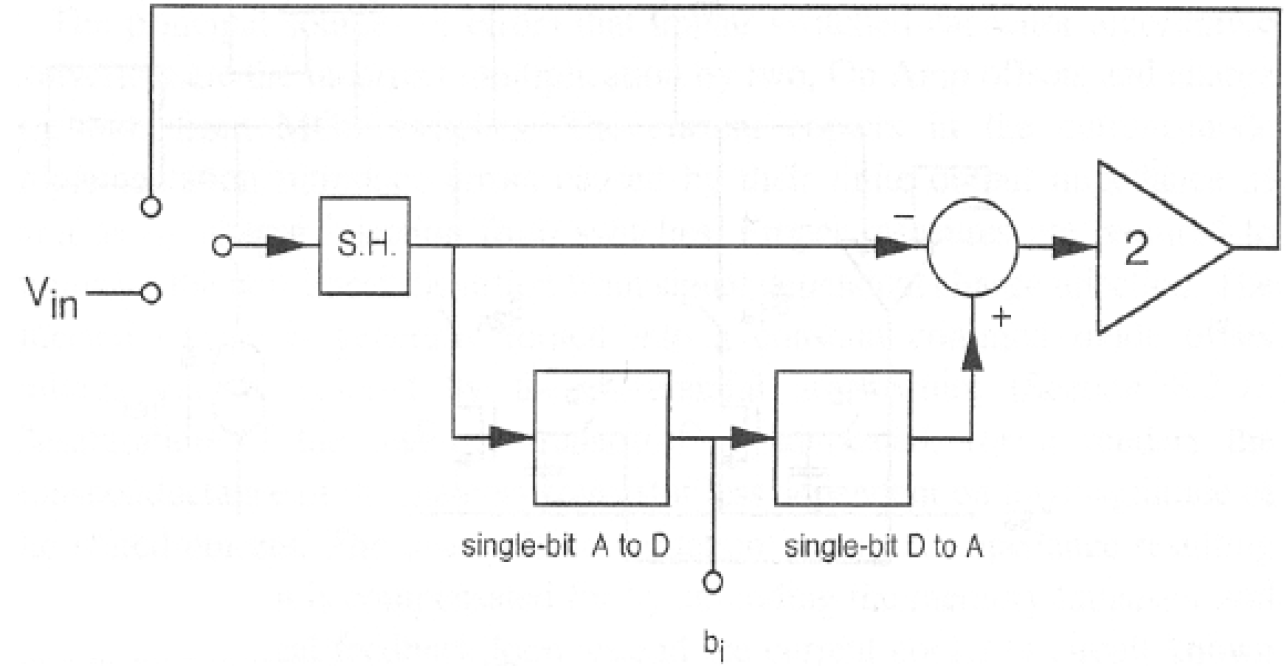
\includegraphics[width=\columnwidth]{images/iterativer_ADC}
\end{minipage}
\hfill
\begin{minipage}[c]{0.58\columnwidth}
    \raggedright
    Reststpannung (Quantisierungsfehler) verdoppeln, damit gleiche Referenzspannung verwendet werden kann 
\end{minipage}

\vspace{0.2cm}

\myul{\textbf{Ablauf einer Wandlung - Iterativer ADC} }

\vspace{0.1cm}

Mit \textbf{jedem Zyklus} (Loop) wird die \textbf{Auflösung um 1 Bit erhöht!}

\begin{minipage}[c]{0.27\columnwidth}
    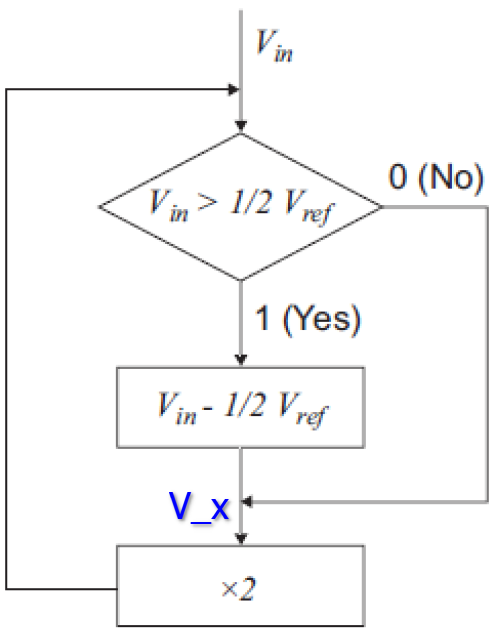
\includegraphics[width=\columnwidth]{images/iterativer_ADC_flussdiagramm.png} 
\end{minipage}
\hfill
\begin{minipage}[c]{0.72\columnwidth}
    \begin{outline}
        \1 Wenn $V_{\rm in} > \frac{V_{\rm ref}}{2}$
            \2 MSB$=1$, $\frac{V_{\rm ref}}{2}$ von $V_{\rm in}$ subtrahieren
            \2 $V_x = V_{\rm in} - \frac{V_{\rm ref}}{2}$
        \1 Wenn $V_{\rm in} < \frac{V_{\rm ref}}{2}$ 
            \2 MSB$=0$
            \2 $V_x = V_{\rm in}$
        \1 $V_x$ verdoppeln zur Bestimmung des nächsten Bits 
    \end{outline}
\end{minipage}


\subsection{Wägeverfahren}

\subsubsection{SAR: Sucessive Approximation Register}

\begin{minipage}[c]{0.35\columnwidth}
    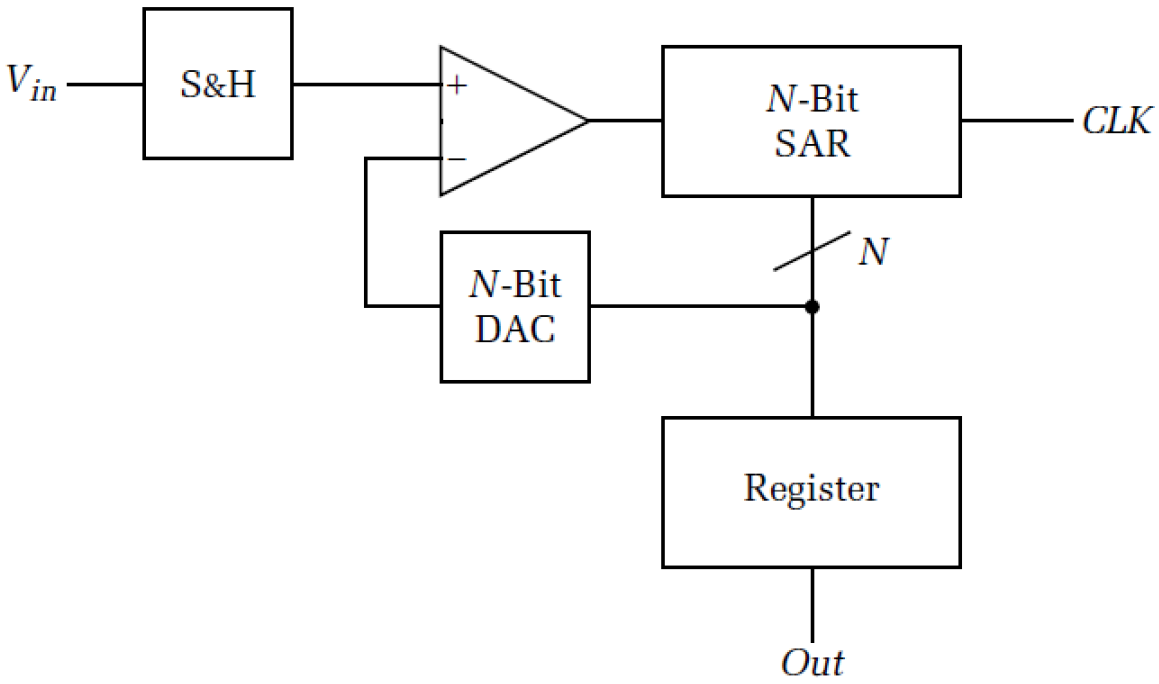
\includegraphics[width=\columnwidth]{images/SAR_ADC.png} 
\end{minipage}
\hfill
\begin{minipage}[c]{0.6\columnwidth}
    \begin{itemize}
        \item DAC-Ausgang nähert sich schrittweise dem Eingangssignal an
        \item Bei $n$ Bit Auflösung dauert eine Wandlung $n$ Zyklen
    \end{itemize}
\end{minipage}


\myul{\textbf{Beispiel Wandlung mit SAR-ADC}}

\vspace{0.1cm}

\begin{minipage}[c]{0.48\columnwidth}
    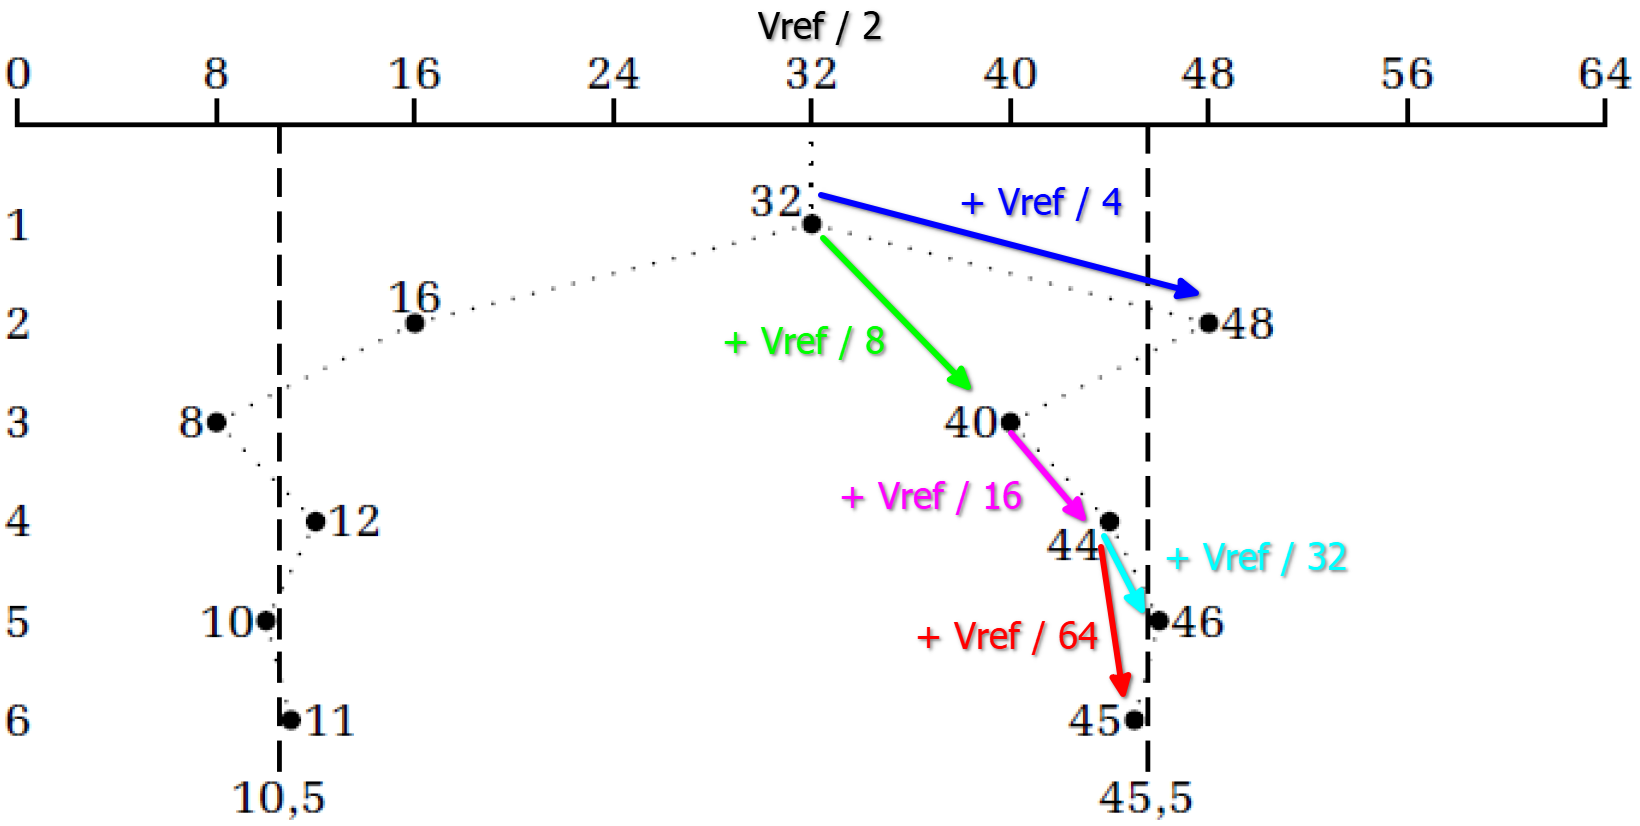
\includegraphics[width=\columnwidth]{images/SAR_ADC_beispiel.png} 
\end{minipage}
\hfill
\begin{minipage}[c]{0.48\columnwidth}
    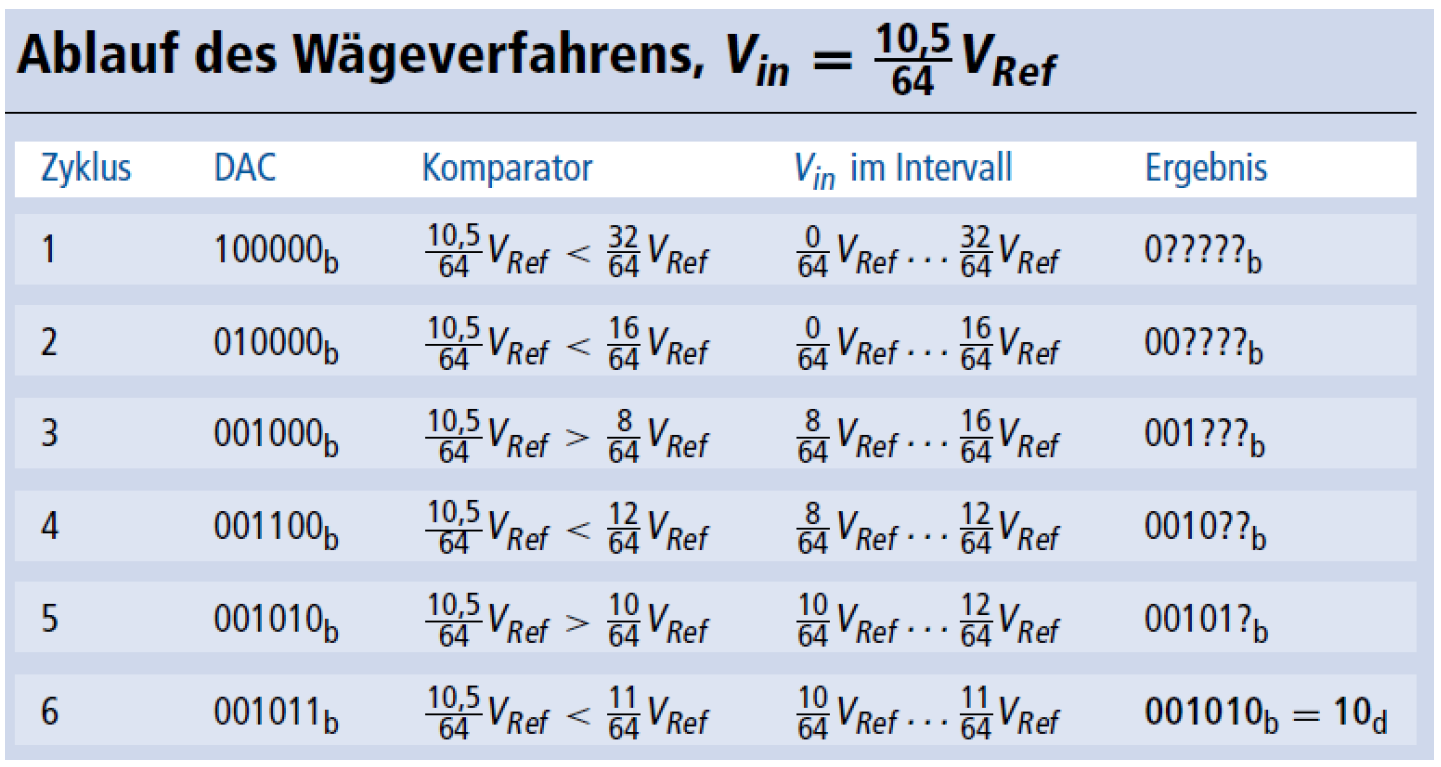
\includegraphics[width=\columnwidth]{images/SAR_ADC_beispiel_2.png} 
\end{minipage}


\subsubsection{SAR mit Switched Capacitor DAC (4 Bit)}

\begin{minipage}[c]{0.48\columnwidth}
    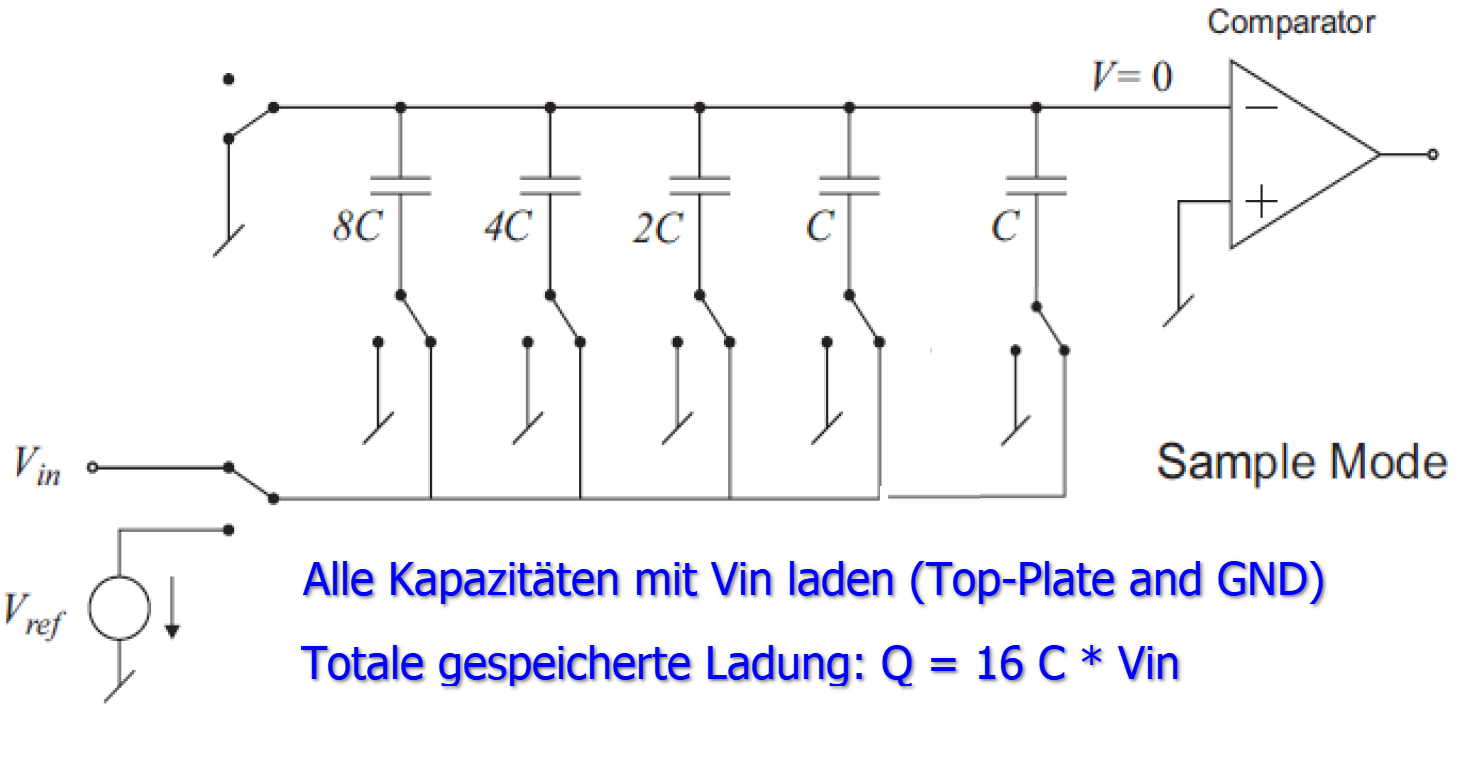
\includegraphics[width=\columnwidth]{images/SAR_switched_capacitor_sample_mode.png}
\end{minipage}
\hfill
\begin{minipage}[c]{0.48\columnwidth}
    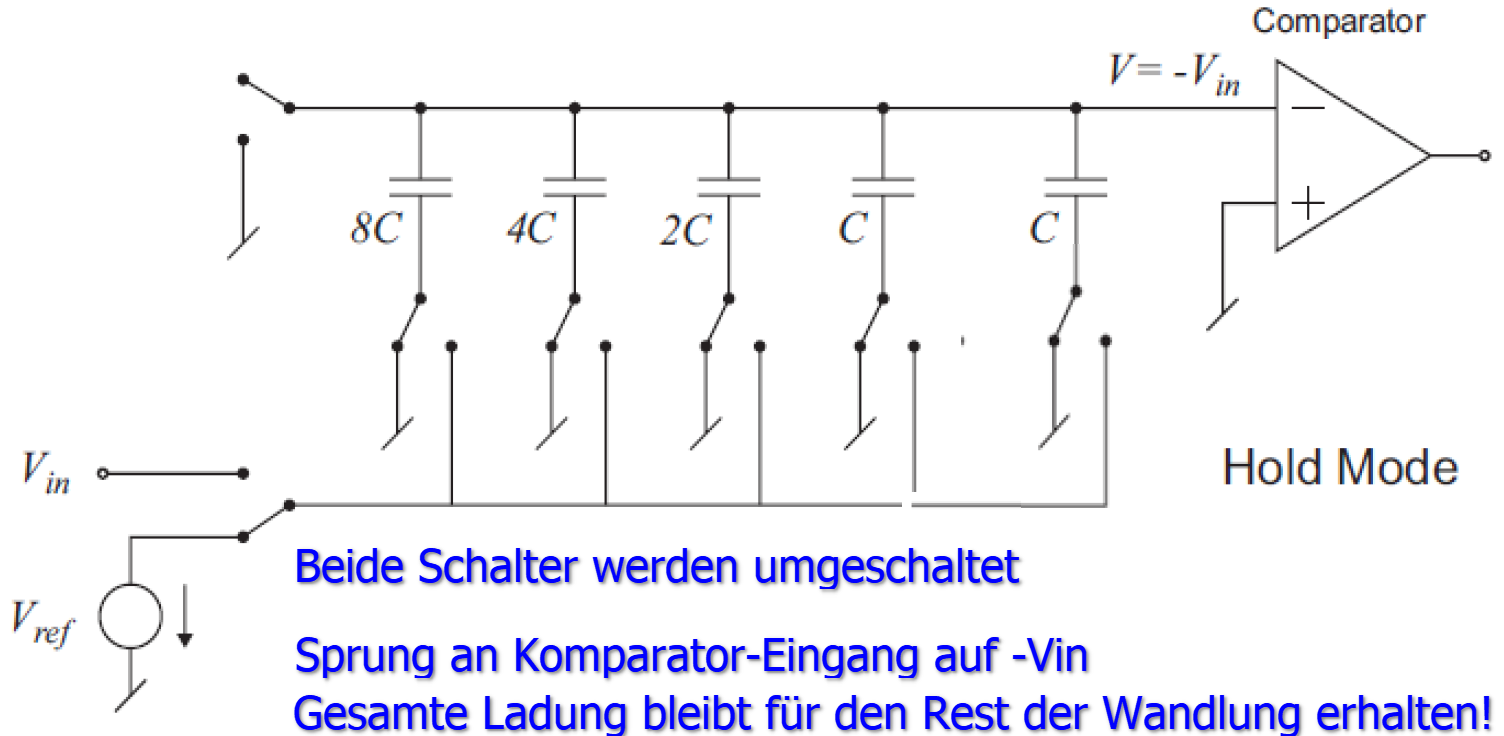
\includegraphics[width=\columnwidth]{images/SAR_switched_capacitor_hold_mode.png}
\end{minipage}

\begin{minipage}[c]{0.45\columnwidth}
    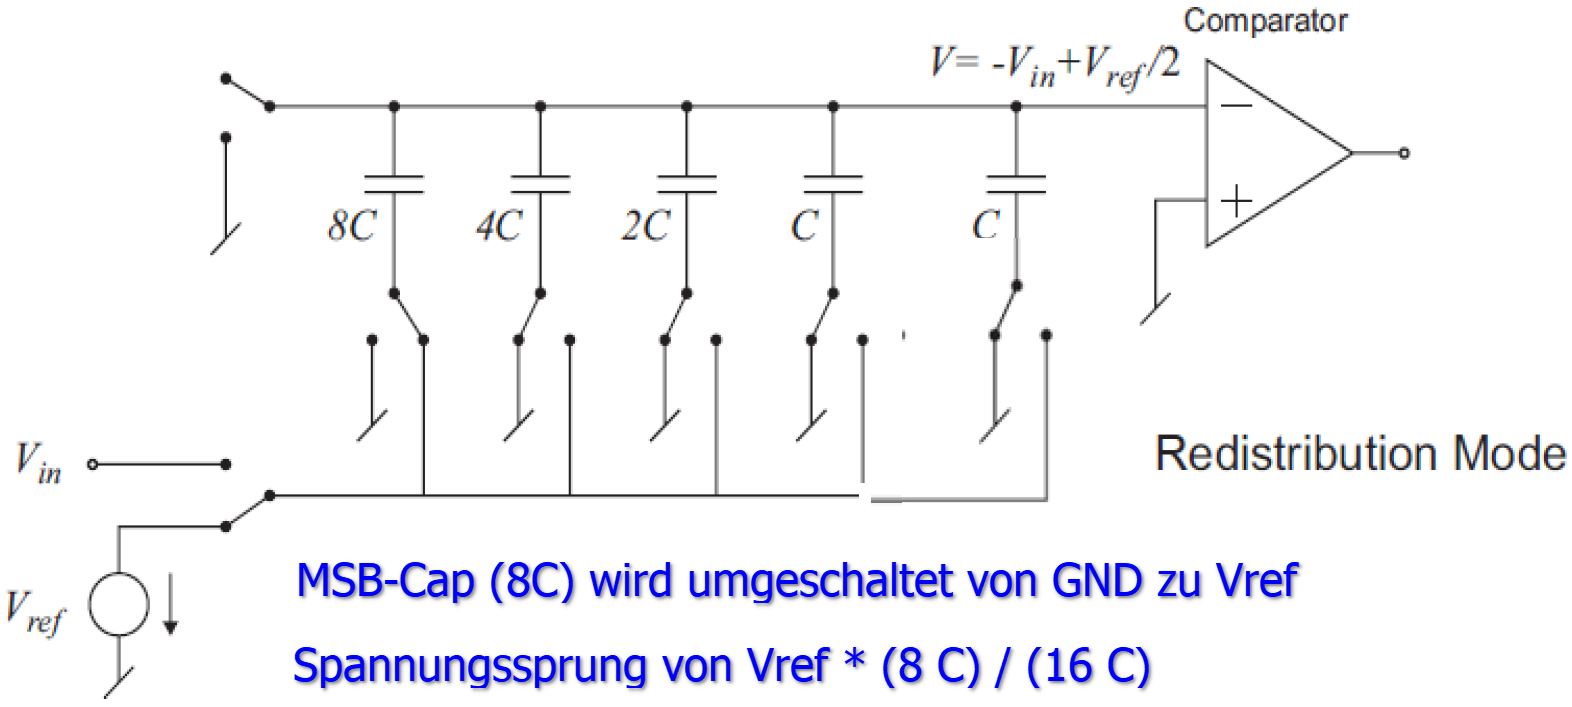
\includegraphics[width=\columnwidth]{images/SAR_switched_capacitor_redistribution_mode.png} 
\end{minipage}
\hfill
\begin{minipage}[c]{0.5\columnwidth}
    Komparator wird ausgewertet:

    \vspace{0.1cm}

    \begin{itemize}
        \item Falls $V < 0 \,V$: Bit = 1 \\
            \textrightarrow\ Schalter bleibt auf $V_{\rm ref}$
        \item Falls $V > 0 \,V$: Bit = 0 \\
            \textrightarrow\ Schalter  zurück auf GND
    \end{itemize}

    \vspace{0.1cm}

    Nächsten Schalter umlegen
\end{minipage}


\subsection{Zählverfahren}

\subsubsection{Grundprinzip: Zählverfahren}

\begin{minipage}[c]{0.4\columnwidth}
    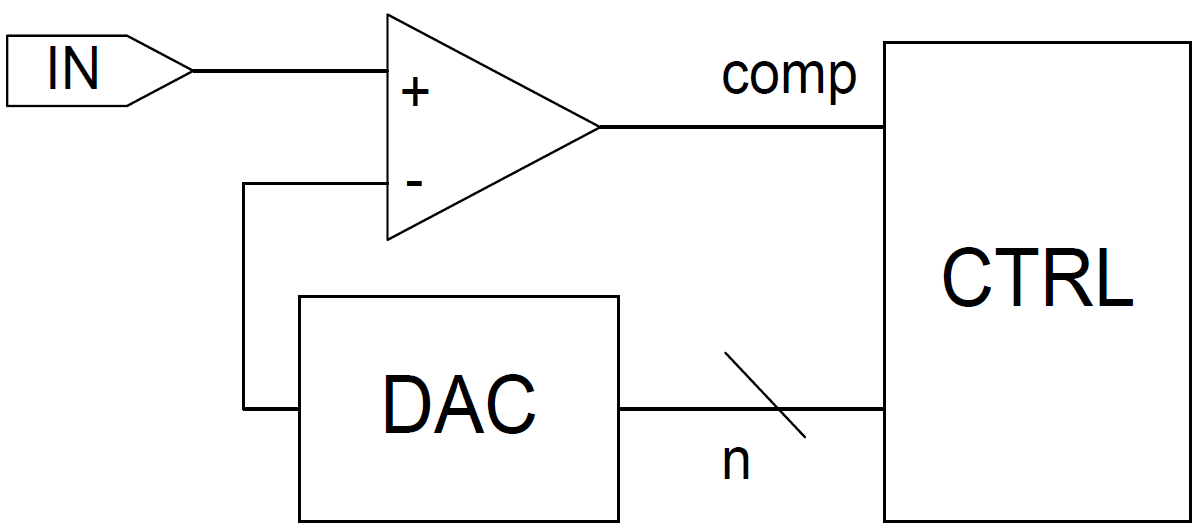
\includegraphics[width=\columnwidth]{images/ADC_zaehlverfahren_grundprinzip.png} 
\end{minipage}
\hfill
\begin{minipage}[c]{0.56\columnwidth}
    \raggedright
    \begin{itemize}
        \item CTRL zählt von $0$ bis $2^n -1$
        \item Zähler stoppt bei $\text{comp} = 0$
        \item \textbf{Zählstand = ADC-Wert} \\
            \textrightarrow\ 'aufgerundet', da DAC-Spannung grösser als $V_{\rm in}$
    \end{itemize}

\end{minipage}


\subsubsection{Single-Slope Wandler}

\begin{minipage}[c]{0.45\columnwidth}
    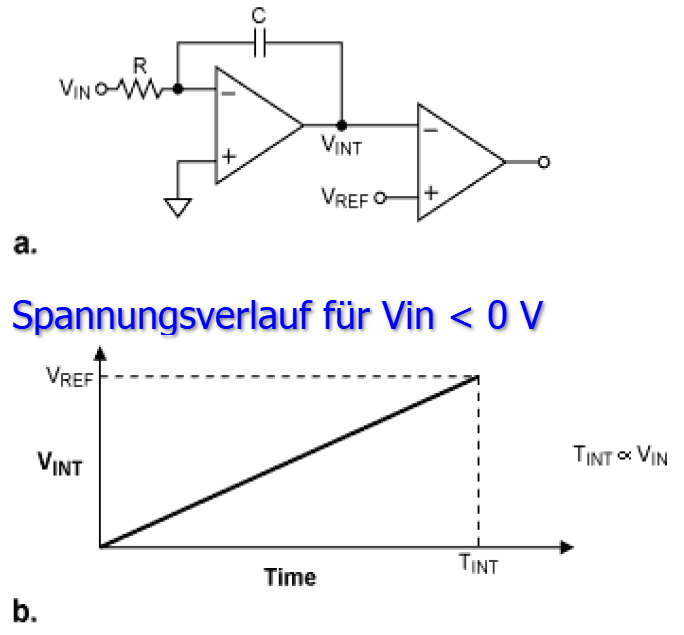
\includegraphics[width=\columnwidth]{images/single_slope_ADC.png} 
\end{minipage}
\hfill
\begin{minipage}[c]{0.52\columnwidth}
    Integration bis $ V_{\rm int}(t) = V_{\rm ref}$ 
    $$ \boxed{ V_{\rm int}(t) = - \frac{V_{\rm in} - A_{\rm GND} }{R \cdot C} \, t  + A_{\rm GND} } $$

    \vspace{0.1cm}

    Integrationszeit $T_{\rm int}$ 
    $$ \boxed{ T_{\rm int} = - \frac{V_{\rm ref} \cdot R \cdot C}{V_{\rm in} - A_{GND}} }$$ 
    $$ \boxed{ V_{\rm in} = - \frac{V_{\rm ref} \cdot R \cdot C}{ T_{\rm int}} } $$ 
\end{minipage}


\subsubsection{Dual-Slope Wandler}

\begin{minipage}[c]{0.42\columnwidth}
    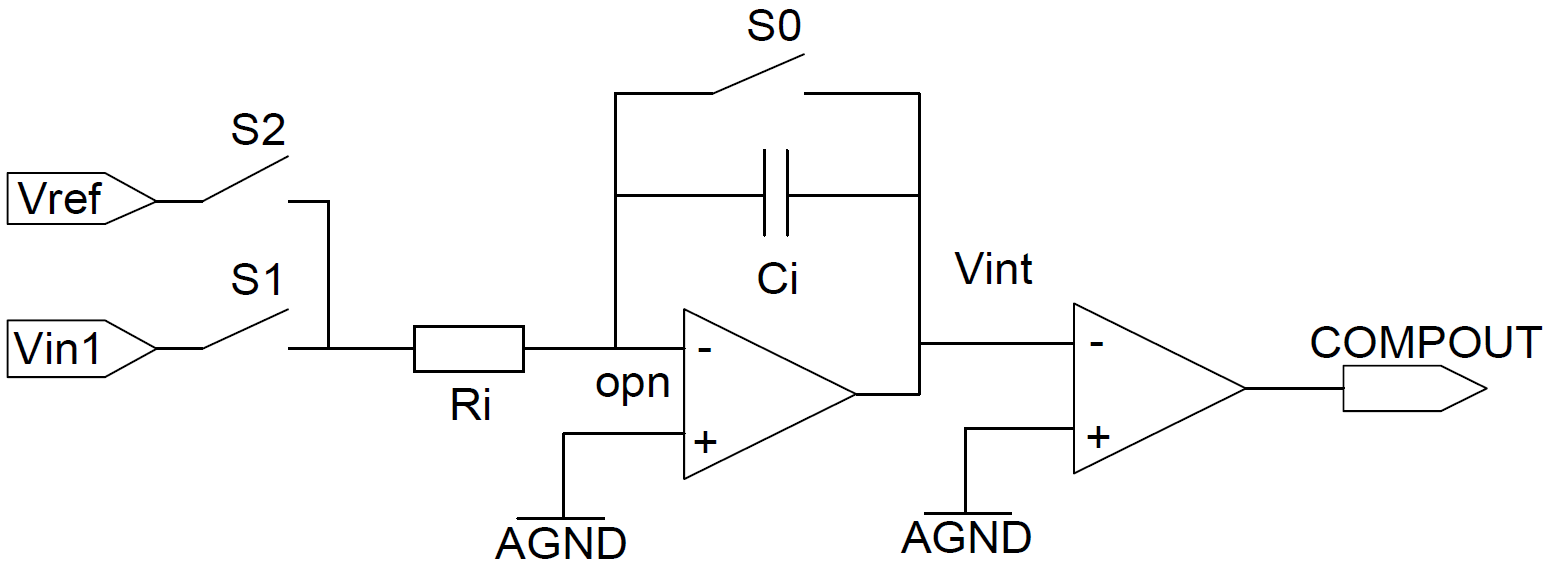
\includegraphics[width=\columnwidth]{images/dual_slope_ADC.png}
\end{minipage}
\hfill
\begin{minipage}[c]{0.27\columnwidth}
    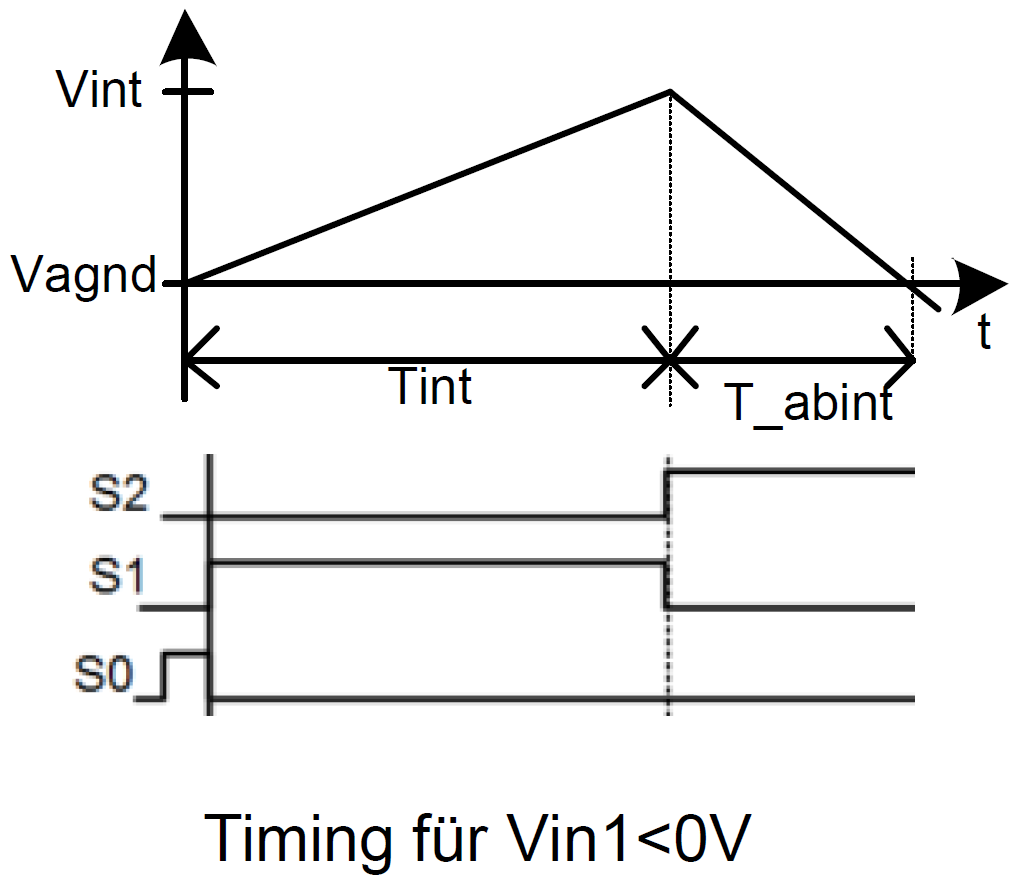
\includegraphics[width=0.83\columnwidth]{images/dual_slope_ADC_timing.png}
\end{minipage}
\hfill
\begin{minipage}[c]{0.29\columnwidth}
    $$ \boxed{ V_{\rm int} = \frac{\overline{V_{\rm in}} \cdot T_{\rm int}}{R_i \cdot C_i} } $$
    $$ \boxed{ V_{\rm abint} = \frac{V_{\rm ref} \cdot T_{\rm abint}}{R_i \cdot C_i}  } $$
\end{minipage}

$$ \boxed{ \text{DC: } V_{\rm int} = A_{\rm GND}- \frac{1}{R_i \cdot C_i} \, (V_{\rm in1}- A_{\rm GND}) \cdot T_{\rm int} }  $$
$$ \boxed{ \Delta V_{\rm abint} = A_{\rm GND} - V_{\rm int} = - \frac{1}{R_i \cdot C_i} \, (V_{\rm ref} - A_{\rm GND}) \cdot T_{\rm abint} } $$ 


\begin{minipage}[c]{0.33\columnwidth}
    $$ \boxed{ T_{\rm abint} = - \frac{V_{\rm in1} \cdot T_{\rm int}}{V_{\rm ref}} } $$ % mit V_AGND??
\end{minipage}
\hfill
\begin{minipage}[c]{0.3\columnwidth}
    $$ \boxed{ V_{\rm in1} = - V_{\rm ref} \frac{T_{\rm abint}}{T_{\rm int}} } $$ % mit V_AGND?
\end{minipage}
\hfill
\begin{minipage}[c]{0.3\columnwidth}
    $$ \boxed{ V_{\rm abint} = - V_{\rm int} } $$ %?
\end{minipage}

\begin{minipage}[c]{0.45\columnwidth}
    $$ \boxed{ -\frac{\overline{V_{\rm in}}}{V_{\rm ref}}= \frac{T_{\rm abint}}{T_{\rm int}} = \frac{n \cdot T_{clk}}{N \cdot T_{clk} } } $$
\end{minipage}
\hfill
\begin{minipage}[c]{0.53\columnwidth}
    $$ \boxed{ V_{\rm int} = \int\limits_0^{T_{\rm int}} - \frac{1}{R_i \cdot C_i} \, V_{\rm in1} + V_{\rm int,0} } $$
\end{minipage}

\vspace{0.2cm}

\myul{\textbf{Frequenzverhalten vom Dual-Slope-Wandler}}

\vspace{0.1cm}

Frequenzen $f = \frac{1}{T}$ , wobei $T$ der Intergrationszeit entspricht, werden perfekt unterdrückt \\
\textrightarrow\ Integrationszeit $T = 20 \, \milli \second$ unterdrückt Netzbrumm von $50 \, \hertz$


\subsubsection{Charge Balancing ADC (Sigma-Delta-Wandler)}

\begin{center}
    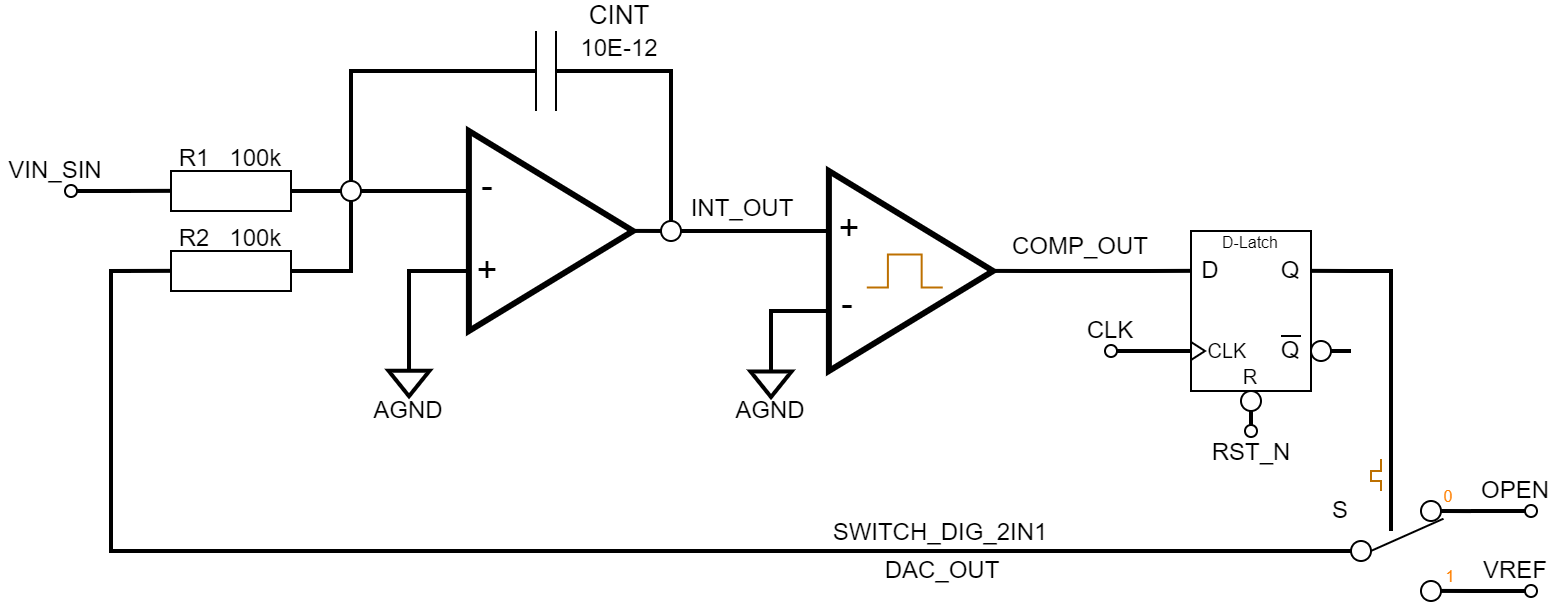
\includegraphics[width=0.8\columnwidth]{images/charge_balancing_ADC.png}
\end{center}


\begin{itemize}
    \item \textbf{Bei jedem Takt} während Aufintegration wird entschieden,
        ob fixe 'Ladungsportion' $Q$ abintegriert wird \textbf{(Schaltschwelle)} \\
        \textrightarrow\ Für CompOut $= 1$ wird für 1 CLK abintegriert
    \item Anzahl 'Ladungsportionen' zählen während $N$ Taktzyklen
    \item \textbf{Integration immer aktiv}
    \item Integrator-Ausgang im Schnitt = Schaltschwelle \textrightarrow\ $\diff Q = 0$
    \item Grosse $N$ \textrightarrow\ Lange Integrationszeit
\end{itemize}

$$ \boxed{ Q = \frac{T_{clk} \cdot V_{\rm ref}}{R_i} }  
    \qquad \boxed{ Q_{\rm int} = \frac{V_{\rm in} \cdot T_{\rm int}}{R_i \cdot C_i} } 
    \qquad \boxed{  \frac{\overline{V_{\rm in}}}{V_{\rm ref}} = \frac{T_{\rm abint}}{T_{\rm int}} = \frac{n}{N} } $$ 
$$ \boxed{ Q_{\rm abint} = \frac{V_{\rm ref} \cdot T_{\rm abint}}{R_i \cdot C_i} = - Q_{\rm int} } $$ 


\subsubsection{Fazit Integrierende Wandler}

\begin{itemize}
    \item In einem Messzyklus wird gleich viel Ladung vom Eingang wie von der Referenzspannung aufintegriert
    \item Sigma-Delta-Wandler können in kürzerer Zeit hohe Auflösungen erreichen als Dual-Slope Wandler 
\end{itemize}


\subsection{Abtastung und Quantisierung}

\begin{tabular}{ll}
\textbf{Aliasing}       & Abgetastetes Signal kann sauber rekonstruiert werden, \\
                        & aber auch schnellere Signale können gleiche Abtastwerte haben \\
\textbf{Abtasttheorem}  & $\bm{f_{\rm abtast} > 2 \cdot f_{\rm signal,max}}$ \\
\textbf{Sample-Hold}    & S-H-Glieder wirken wie Tiefpassfilter, indem das Spektrum mit \\
                        & einer sinc-Funktion $(\sin(x)/x)$ gewichtet wird  \\
                        & \textrightarrow\ ALLE Frequenzen $> 0 \, \hertz$ werden durch S-H gedämpft! \\
                        & (gutes S-H = wenig Dämpfung)
\end{tabular}


\subsection{Lineares Modell der Quantisierung / SNR}

\subsubsection{Voraussetungen für lineare Modellierung der Quantisierung}

\begin{itemize}
    \item Anzahl der Bits $N$ ist gross
    \item ADC wird nicht übersteuert $(V_{\rm refn} < V_{\rm in} < V_{\rm refp})$
    \item Alle Spannungen kommen in Eingangssignal gleich oft vor
    \item Analoges Eingangssignal variiert sehr schnell
\end{itemize}


\subsubsection{Signal-Rausch-Abstand (SNR)}

\begin{itemize}
    \item \textbf{SNR:} Verhältnis Signalleistung zu Quantisierungsrauschen \textbf{in dB}
    \item ENOB: Effevtive Number of Bits
\end{itemize}

\vspace{0.2cm}

\renewcommand{\arraystretch}{1.5}
\begin{tabular}{ll}
    Leistung Quantisierungsrauschen & $P_Q = \frac{q^2}{12}$                                            \\
    Leistung Eingangssignal         & $P_S = 2^{2 \cdot n - 3} \cdot q^2$                               \\
    SNR                             & $1.76 + n \cdot 6.02$ mit $n =$ \# Bits                           \\
    ENOB                            & $\mathrm{ENOB} = \frac{\mathrm{SNR_{\deci \bel}} - 1.76}{6.02}$ 
\end{tabular}
\renewcommand{\arraystretch}{1}

\vspace{0.2cm}

\textbf{ \textrightarrow\ Pro Bit erhöht sich SNR um 6.02 dB}
 
 
\subsection{Kennwerte von ADCs}

\begin{center}
    \begin{tabular}{lccc}
        \toprule
                                    & \textbf{Pipelined}    & \textbf{Wägeverfahren}    & \textbf{Sigma-Delta}      \\
        \midrule
        \textbf{Auflösung}          & niedrig               & mittel                    & hoch                      \\  
                                    & 8 - 14 Bit            & 8 - 20 Bit                & 16 - 24 Bit               \\
        \midrule
        \textbf{Umsetzungsrate}     & sehr hoch             & mittel-hoch               & niedrig-mittel            \\
                                    & bis zu 4 GSa          & bis zu 10 MHz             & 1 Hz - 100 kHz            \\
        \midrule
        \textbf{Leistungsaufnahme}  & sehr hoch             & mittel                    & niedrig                   \\
                                    & bis zu 3 W            & 1 - 200 mW                & 0.2 - 10 mW               \\
        \bottomrule
    \end{tabular}
\end{center}


		\section{Halbleiter}

\subsubsection{Leitfähigkeit / elektrischer Widerstand}

\begin{minipage}[t]{0.48\columnwidth}
	\myul{\textbf{Leitfähigkeit $\bm{\kappa}$}}
	$$ \boxed{ \kappa = \frac{1}{\rho} = n \cdot q \cdot \mu } $$
\end{minipage}
\hfill
\begin{minipage}[t]{0.48\columnwidth}
	\myul{\textbf{(Leiter-)Widerstand}}
	$$ \boxed{ R = \frac{\rho \cdot l}{A} = \frac{l}{ \kappa \cdot A} } $$
\end{minipage}

\vspace{0.2cm}

\myul{\textbf{Temperaturabhängigkeit (1. Näherung linear)}}
$$ \boxed{ \rho(T) = \rho(T_0) \cdot (1  + \alpha(T - T_0)) } $$


\begin{tabular}{clc}
	$n$ 						& Ladungsträgerdichte 									& 												\\
	$q$ 						& Elementarladung $q = 1.6 \cdot 10^{-19} \, \coulomb$ 	& $[q] = \coulomb$								\\
	$l$ 						& Läge des Leiters 										& $[l] = \meter$ 								\\
	$A$ 						& Querschnittsfläche des Leiters 						& $[A] = \meter^2$ 								\\
	$\mu$ 						& Beweglichkeit der Ladungsträger 						& 												\\
	$\alpha$ 					& Temperaturkoeffizient 								& $[\alpha] = \frac{1}{\kelvin}$ 				\\
	$\kappa = \frac{1}{\rho}$ 	& Spez. Leitfähigkeit bzw. spez. Widerstand 			& $[\kappa] = \frac{\meter}{\ohm \cdot \milli \meter}$
\end{tabular}


\subsubsection{Elektrische Eigenschaften von (Halb-)Leitern / Isolatoren}

\begin{tabular}{ll}
	Leiter 		& \textbf{positiver} Temperaturkoeffizent $\alpha$ 									\\
				& Leitfähigkeit Metalle: $10^6 \ldots 10^8 \, \frac{\siemens}{\meter}$ (2 Dekaden) 	\\
	Halbleiter 	& \textbf{negativer} Temperaturkoeffizent $\alpha$ 									\\
				& \textbf{Dotierung} Verändert Leitfähigkeit (10 Dekaden) 							\\
	Isolatoren 	& Kein Temperaturkoeffizent $\alpha$ 
\end{tabular}


\subsection{Dotierung von Halbleitern}

Unter \textbf{Dotierung} versteht man das Einbringen von Fremdatomen ins Kristallgitter des Halbleiters (z.B. von Silizium)

\begin{center}
	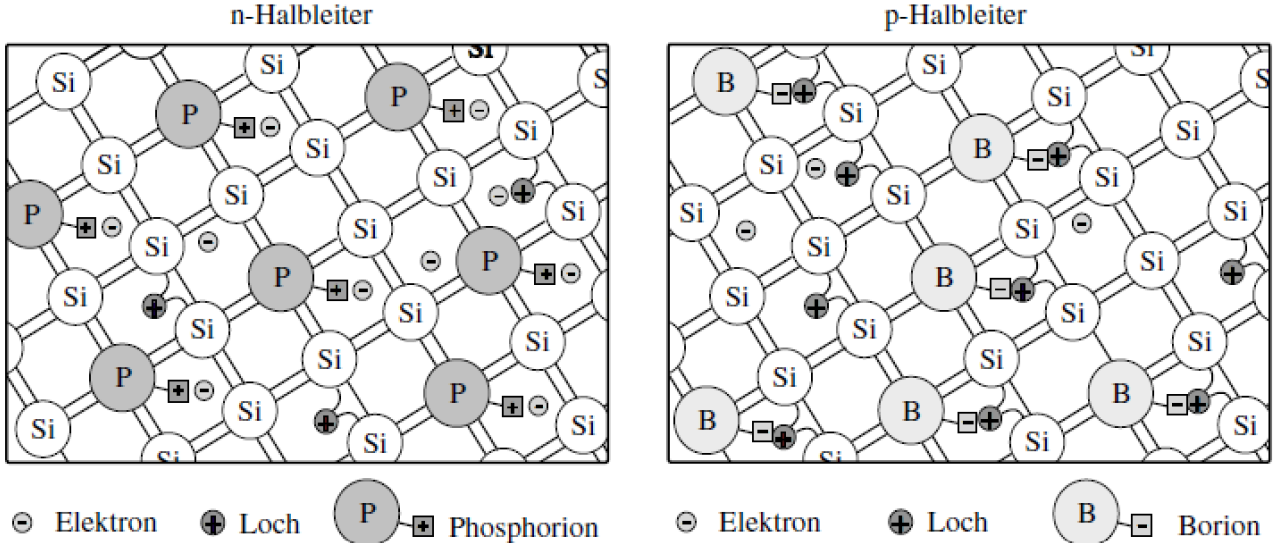
\includegraphics[width=0.75\columnwidth]{images/dotierung.png}
\end{center}


\begin{tabular}{ll}
	\textbf{n-Dotierung} 	& Zufügen von Atomen mit 5 Elektronen 		\\
							& \textrightarrow\ Elektronen-Überschuss 	\\
	\textbf{p-Dotierung} 	& Zufügen von Atomen mit 3 Elektronen 		\\
							& \textrightarrow\ Löcher-Überschuss
\end{tabular}

\vspace{0.2cm}

\textrightarrow\ p-Dotierung ist immer schlechter (geringere Leitfähigkeit), da Elektronen fehlen


\subsection{pn-Übergang}

\begin{tabular}{| ll | ll |}
	\hline
	P-Anschluss: 	& Anode 	& RLZ: 	& Raumladungszone	\\
	N-Anschluss: 	& Kathode 	& \el 	& Elektron 			\\
	\hline
\end{tabular}


\subsubsection{pn-Übergang ohne äussere Spannung}

\begin{minipage}[c]{0.3\columnwidth}
	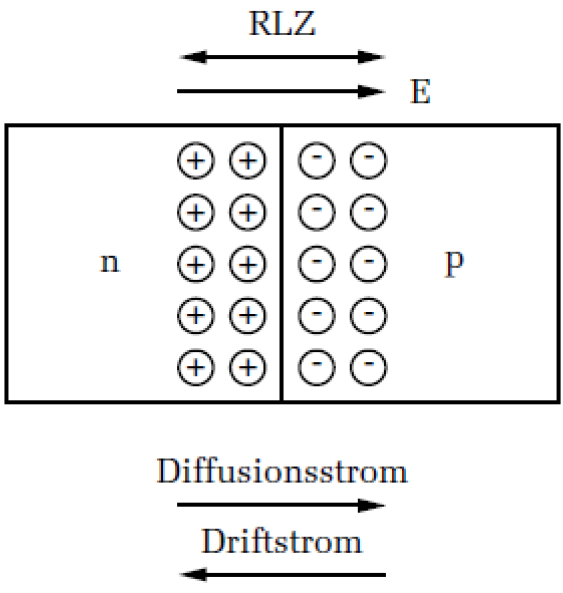
\includegraphics[width=\columnwidth]{images/pn-uebergang.png}
\end{minipage}
\hfill
\begin{minipage}[c]{0.65\columnwidth}
	\textbf{Diffusionsstrom: Dichte-Ausgleich} \\
	\el diffundieren in p-Zone, Löcher in n-Zone

	\vspace{0.2cm}

	\textbf{Driftstrom: Durch elektrisches Feld} \\
	\el von positiver Spannung in n-Zone angezogen \\
	\textrightarrow\ Es entsteht ein Gleichgewicht!

	\vspace{0.2cm}

	Zwischen p- und n-Bereich entsteht isolierende \textbf{RLZ}
\end{minipage}


		\section{Dioden}

\begin{tabular}{ll}
    Kleinsignal-Ersatzschaltung:    &  Kleinsignal-Widerstand $r_d$ \\
    Grosssignal-Ersatzschaltung:    & Spannungsquelle + $r_d$
\end{tabular}


\subsection{Aufbau}

\begin{minipage}[c]{0.4\columnwidth}
    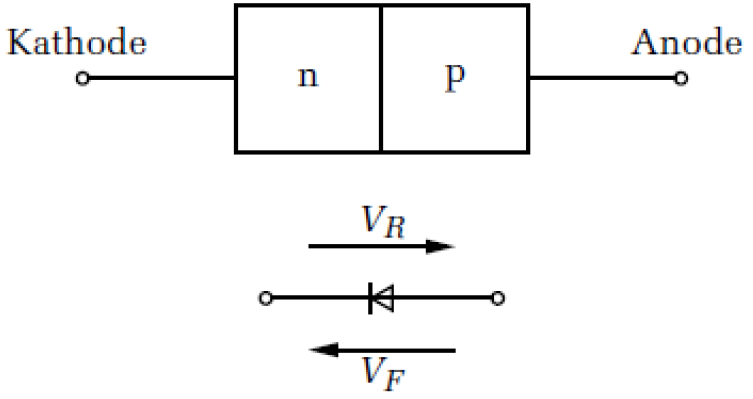
\includegraphics[width=\columnwidth]{images/diode.png}
\end{minipage}
\hfill
\begin{minipage}[c]{0.55\columnwidth}
    \raggedright
    Positiver Strom in Flussrichtung    \\
    (Anode \textrightarrow\ Kathode)

    \vspace{0.2cm}

    \textbf{Stromverdoppelung alle $\bm{20 \milli \volt}$}
\end{minipage}

\vspace{0.2cm}

\begin{minipage}[c]{0.3\columnwidth}
    \begin{center}
        Für $ V_d < 200 \, \milli \volt $
        $$ \boxed{ I_D = I_S \Big( e^{\frac{V_D}{n \cdot V_T}} -1 \Big)} $$
    \end{center}
\end{minipage}
\hfill
\begin{minipage}[c]{0.65\columnwidth}
    \begin{center}
        Für $ V_d > 200 \, \milli \volt $
        $$ \boxed{ I_D = I_S \cdot e^{\frac{V_D}{n \cdot V_T}}} \qquad \bm{V_T} = \frac{k_B \cdot T}{q} \bm{ \approx 25 \, \milli \volt} $$
    \end{center}
\end{minipage}

\vspace{0.3cm}

\begin{tabular}{ll}
    $I_S$   & Sättigungsstrom $(\pico \ampere \ldots \nano \ampere)$                        \\
    $n$     & Emissionskoeffizient $1 < n < 2$                                              \\
    $k_B$   & Boltzmann-Konstante $k_B = 1.38 \cdot 10^{-23} \, \frac{\joule}{\kelvin} $    \\
    $T$     & \textbf{Absolute} Temperatur in $\kelvin$
\end{tabular}


\subsection{Ersatzschaltungen}

\subsubsection{Grosssignal-Ersatzschaltung}

\begin{minipage}[c]{0.46\columnwidth}
    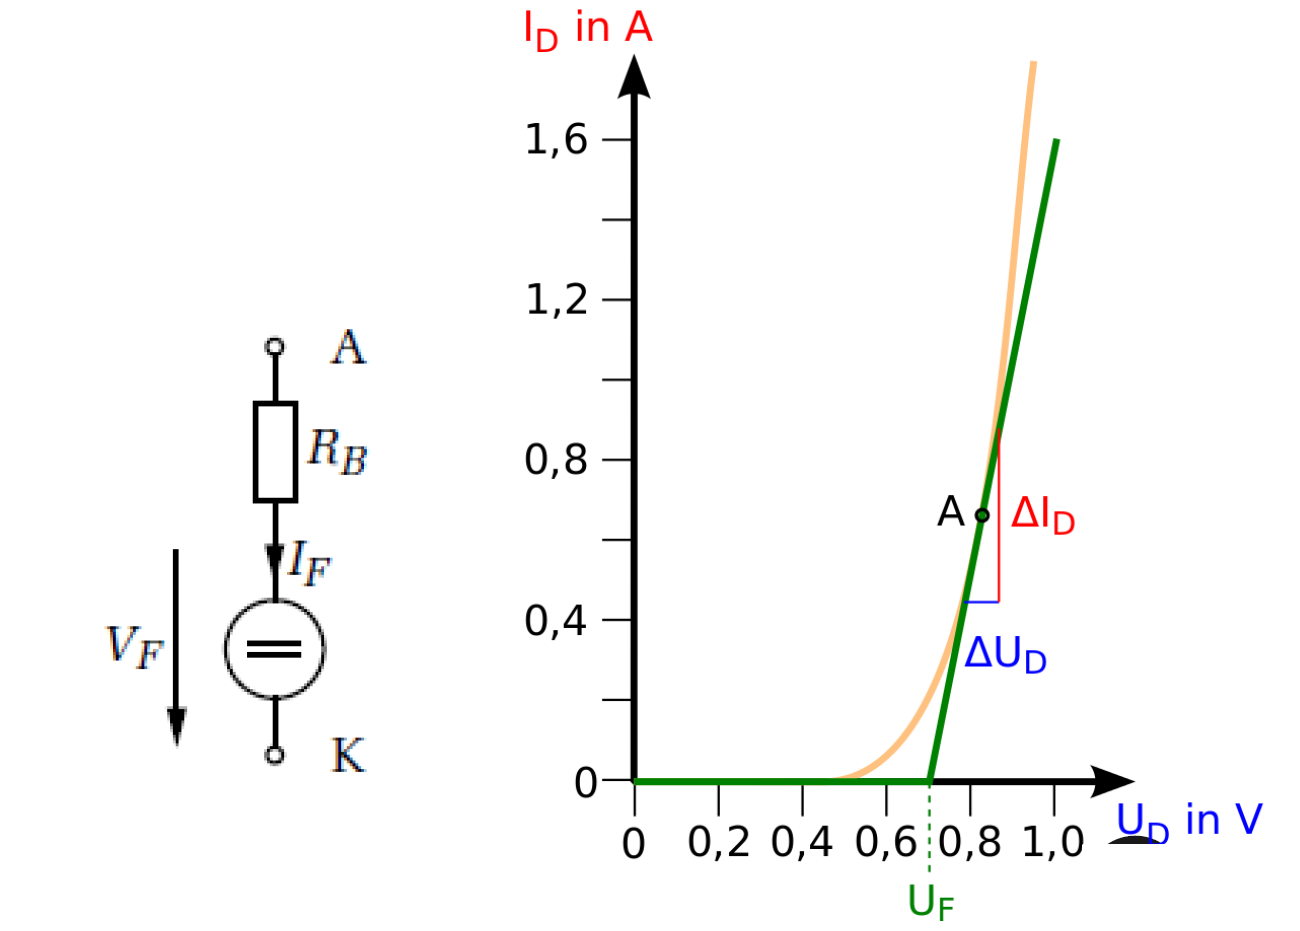
\includegraphics[width=\columnwidth]{images/vereinfachte_reale_diode.png}
\end{minipage}
\hfill
\begin{minipage}[c]{0.53\columnwidth}
    \myul{\textbf{Tangente im Arbeitspunkt}}

    \vspace{0.1cm}

    \begin{tabular}{ll}
        $r_d$:  & Steigung der Kennlinie \\
        $V_F$:  & Verlängerung Tangente  \\
                & (Schnittpunkt)
    \end{tabular}

    $$ \boxed{ g = \frac{1}{r_d} = \frac{\diff I_D}{\diff V_D} } $$
    $$ \boxed{ g = \frac{1}{n \cdot V_T} I_S \cdot e^{\frac{V_D}{n \cdot V_T}} = \frac{I}{n \cdot V_T} } $$
\end{minipage}


\subsubsection{Kleinsignalersatzschaltung}

Nur Widerstand $r_d$ \textbf{ohne Spannungsquelle}

\vspace{0.1cm}

\begin{tabular}{ll}
    Diode sperrt:   & $r_d = \infty$            \\
    Diode leitet:   & $r_d$ gemäss Kennlinie
\end{tabular}


\subsection{Temperaturverhalten}

\begin{minipage}[c]{0.35\columnwidth}
    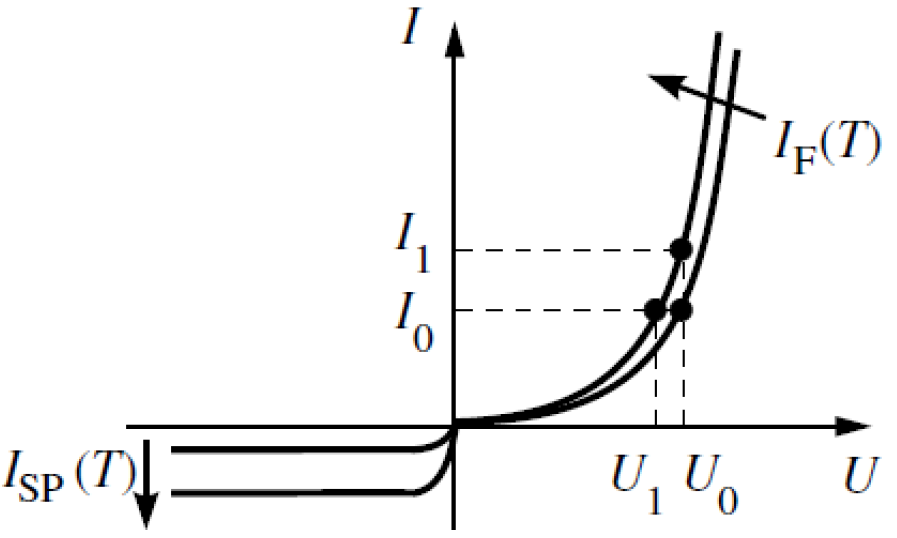
\includegraphics[width=\columnwidth]{images/diode_temperaturverhalten.png}
\end{minipage}
\hfill
\begin{minipage}[c]{0.62\columnwidth}
    \raggedright
    \myul{\textbf{Leitender Bereich}}

    \vspace{0.1cm}

    $$ \boxed{ \frac{\diff V_F}{\diff T} = -2 \, \frac{\milli \volt}{\kelvin} \quad \text{@ }  I = \const } $$

    \vspace{0.1cm}

    \textbf{ \textrightarrow\ Diodenspannung nimmt pro $\bm{\celsius}$ um $\bm{2 \, \milli \volt}$ ab}
\end{minipage}

\vspace{0.2cm}

\myul{\textbf{Sperrender Bereich}}

\vspace{0.1cm}

\begin{itemize}
    \item Sperrstrom-Zunahme erfolgt exponentiell mit der Temperatur
    \item Verdoppelung des Sperrstroms bei Temperatur-Erhöhung um $10 \, \celsius$ \\
        \textrightarrow\ Verdoppelung der Ausfallrate!
\end{itemize}


\subsubsection{Thermische Spezifikation}

\begin{itemize}
    \item \textbf{Temperatur von Silizium-Halbleitern darf $\bm{170 \celsius}$ nicht überschreiten}
    \item Bauform (Gehäuse) wird abhängig vom max. Strom bzw. der zulässigen Verlustleistung gewählt
    \item Mit grösserer Siliziumfläche erhöht sich auch der Sättigungssperrstrom $I_S$
    \item Thermischer Widerstand $R_{\theta}$ in $\celsius / \watt$ gibt an, wieviel sich Halbleiter mit Verlustleistung erwärmt 
\end{itemize}


\subsection{Dioden bei negativer Spannung}

\begin{minipage}[c]{0.35\columnwidth}
    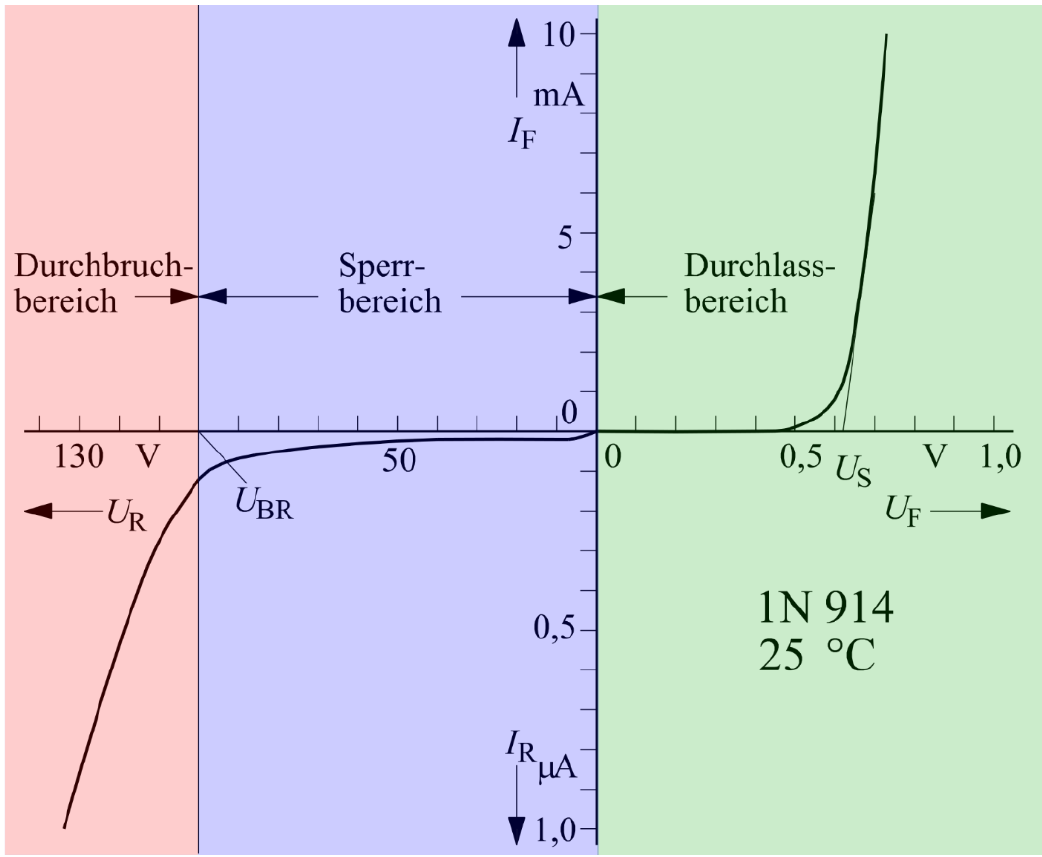
\includegraphics[width=\columnwidth]{images/diodenbereiche.png}
\end{minipage}
\hfill
\begin{minipage}[c]{0.62\columnwidth}
    \textbf{Diodendurchbruch @ $\bm{V_{\rm BR}$}}

    \vspace{0.1cm}

    Bei hoher negativer Sperrspannung steigt Sperrstrom zunächst langsam und dann schlagartig an. \\
    Gleichrichterdioden: $V_{\rm BR} \approx 50 \, \volt \, \ldots \, 1000 \, \volt $
\end{minipage}


\subsection{Diodenschaltungen}

\subsubsection{Diode mit Seriewiderstand}


\begin{minipage}[c]{0.4\columnwidth}
    \begin{center}
        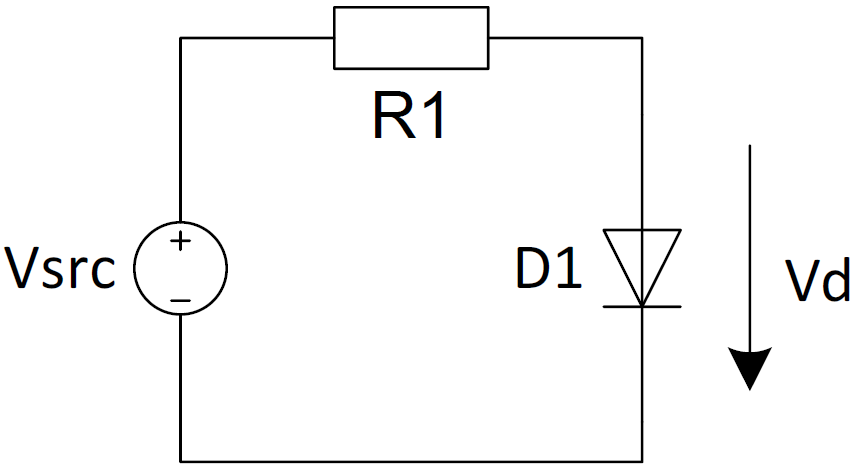
\includegraphics[width=0.8\columnwidth]{images/diode_mit_seriewiderstand.png}

        \vspace{0.2cm}

        \cbl{\textbf{Widerstandsgerade:} }
        $$I_{KS} = \frac{V_{SRC}}{R_1} \quad  (\text{@ } V_d = 0) $$
        $$ U_0 = V_{\rm SRC} \quad (\text{@ } I = 0) $$
    \end{center}
\end{minipage}
\hfill
\begin{minipage}[c]{0.5\columnwidth}
    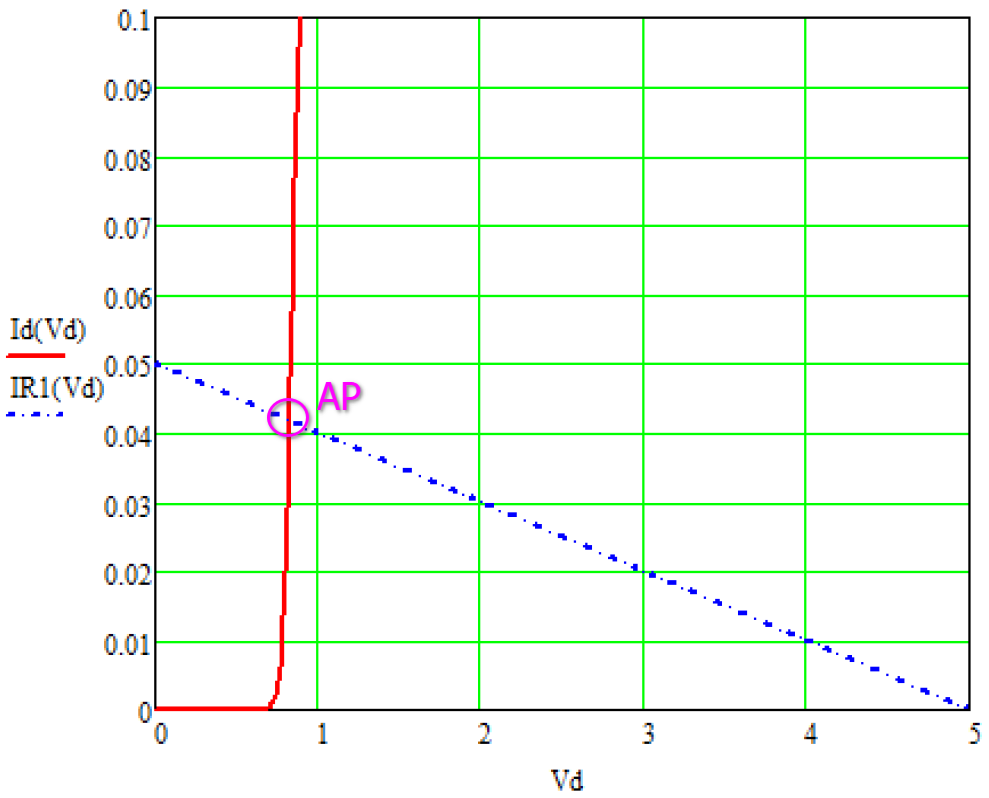
\includegraphics[width=\columnwidth]{images/diode_mit_seriewiderstand_kennlinie.png}
\end{minipage}


\subsubsection{Einweg-Gleichrichter}

\begin{minipage}[c]{0.35\columnwidth}
    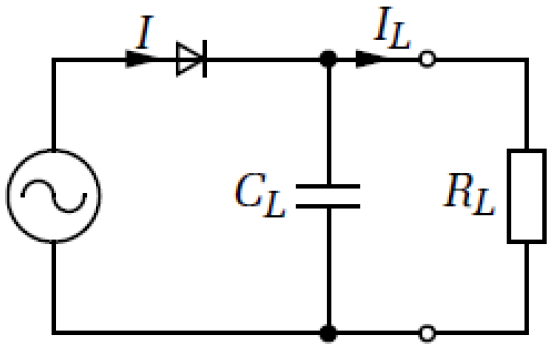
\includegraphics[width=\columnwidth]{images/einweggleichrichter.png}
\end{minipage}
\hfill
\begin{minipage}[c]{0.6\columnwidth}
    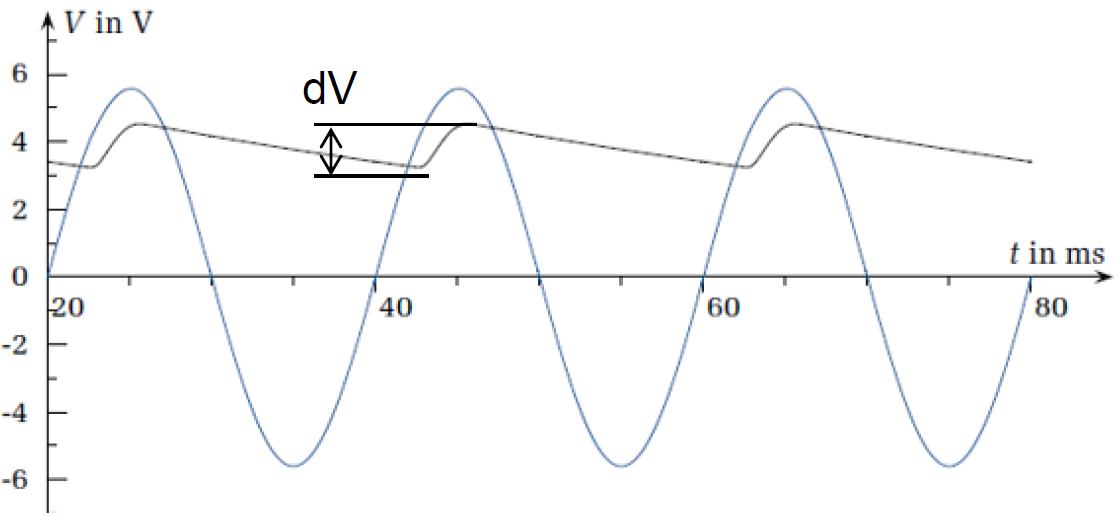
\includegraphics[width=\columnwidth]{images/einweggleichrichter_spannung.png}
\end{minipage}

\vspace{0.2cm}

\begin{minipage}[c]{0.52\columnwidth}
    \begin{tabular}{@{}ll@{}}
        Diode leitet:   & $V_{\rm out}= V_{\rm in} - V_D$               \\
        Diode sperrt:   & $V_{\rm out}= 0 \, \volt$                     \\
        Entladen:       & $C$ wird über $R$ entladen                    \\
                        & $V_{\rm out}(t) = e^{- \frac{t}{R \cdot C} }$ \\
        Rippelspannung: & $\diff V$                                     \\
        Laststrom:      & $I_0 = \frac{V_{\rm in}}{R_L}$
    \end{tabular}
\end{minipage}
\hfill
\begin{minipage}[c]{0.4\columnwidth}
    \raggedright
    Je kleiner die Rippel-Spannung,

    \vspace{0.1cm}

    \begin{itemize}
        \item desto kürzer die Aufladezeit
        \item desto grösser der maximale Strom
    \end{itemize}
\end{minipage}


\subsubsection{Brücken- / Vollwellengleichrichter}

\begin{minipage}[c]{0.45\columnwidth}
    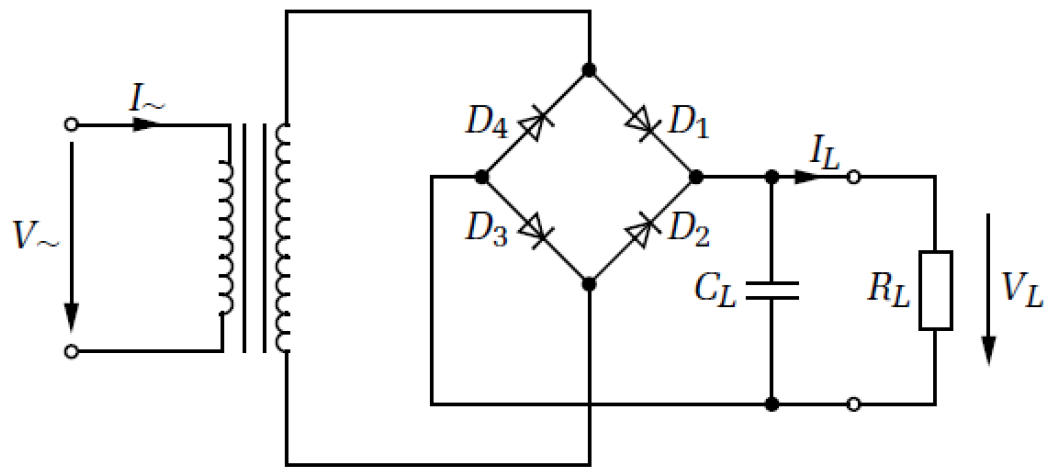
\includegraphics[width=\columnwidth]{images/brueckengleichrichter.png}
\end{minipage}
\hfill
\begin{minipage}[c]{0.52\columnwidth}
    \begin{itemize}
        \item[+] Nur halbe Rippel-Spannung
        \item[+] symm. Netzbelastung
        \item[-] Doppelter Spannungsverlust (2 Dioden)
    \end{itemize}
\end{minipage}



\subsection{Spannungsvervielfacher}

\subsubsection{Dickson Charge Pump $\bm{(N = 2)}$}

\begin{minipage}[c]{0.5\columnwidth}
    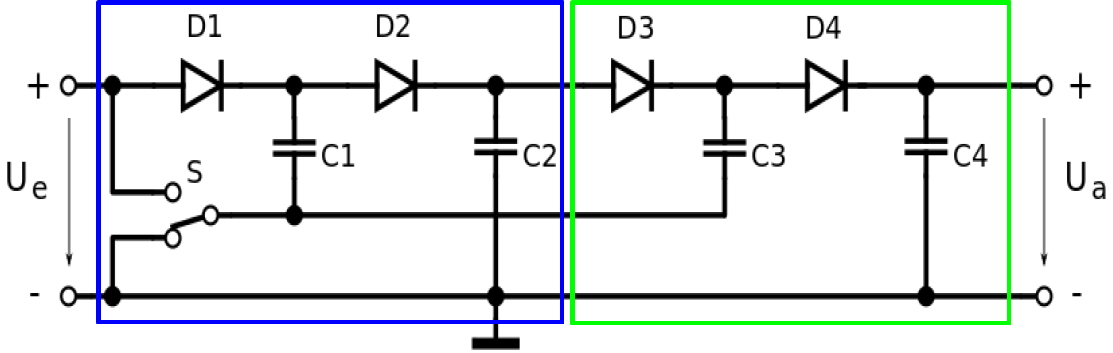
\includegraphics[width=\columnwidth]{images/dickson_charge_pump.png} 
\end{minipage}
\hfill
\begin{minipage}[c]{0.48\columnwidth}
    Aus kleiner DC-Spannung wird grössere DC-Spannung erzeugt 
    $$ \boxed{ U_a = (N+1) \cdot U_e - N \cdot 2 \cdot U_D} $$
\end{minipage}


\subsubsection{Villard-Schaltung (Spannungsverdoppler)}

\begin{minipage}[c]{0.4\columnwidth}
    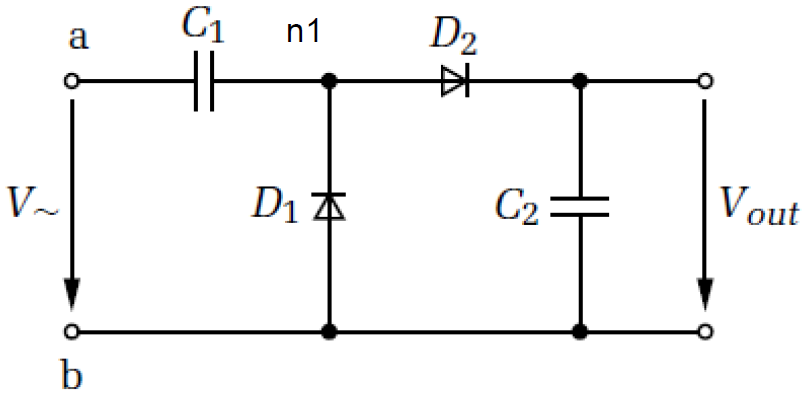
\includegraphics[width=\columnwidth]{images/villard_schaltung.png}
\end{minipage}
\hfill
\begin{minipage}[c]{0.58\columnwidth}
    $$ \boxed{ V_{\rm out} = 2 \cdot V_{\rm in} - 2 \cdot V_D} $$

    \begin{itemize}
        \item Verfielfacht AC-Spannungen
        \item $V_{\rm in} > 0$ Strom über $D_2$ in Last
        \item $V_{\rm in} < 0$ Strom über $D_1$ und $C_1$
        \item Spannung an $n1$ wird angehoben 
    \end{itemize}
\end{minipage}


\subsection{Spezielle Dioden}

\subsubsection{Schottky-Dioden}

\begin{minipage}[c]{0.3\columnwidth}
    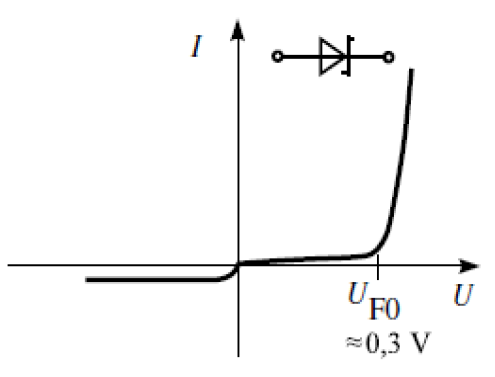
\includegraphics[width=\columnwidth]{images/schottky_diode.png}
\end{minipage}
\hfill
\begin{minipage}[c]{0.68\columnwidth}
    \raggedright
    
    \begin{itemize}
        \item \textbf{Flussspannung:} $ \bm{V_{\rm F0} \approx 0.3 \, \volt}$
        \item Viel höherer Sättigungs-Sperrstrom als Si-Diode \\
            \textrightarrow\ Für kleine Ströme ok
        \item Stromanstieg weniger steil als bei Si-Diode 
        \item Grössere Leckströme
    \end{itemize}
\end{minipage}


\subsubsection{Zener-Dioden / Z-Dioden}

\begin{minipage}[c]{0.4\columnwidth}
    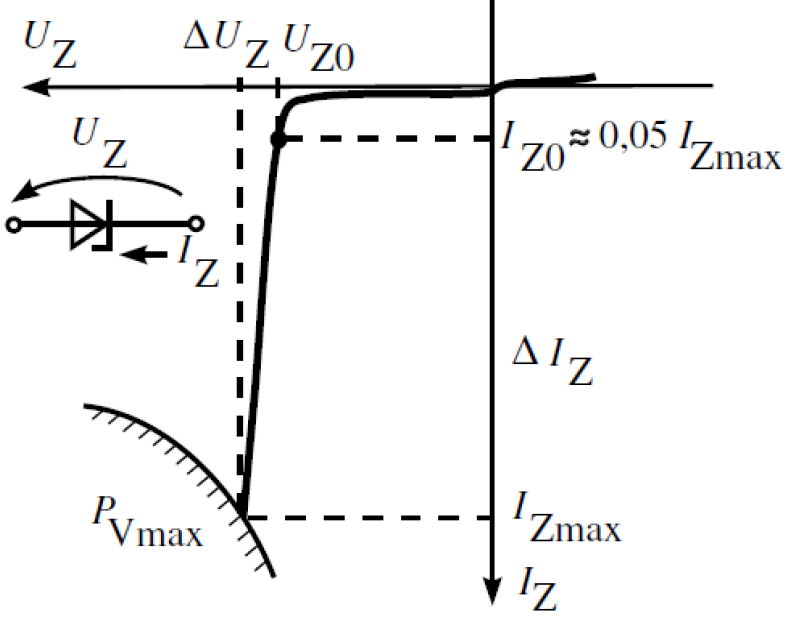
\includegraphics[width=\columnwidth]{images/zener_diode.png}
\end{minipage}
\hfill
\begin{minipage}[c]{0.45\columnwidth}
    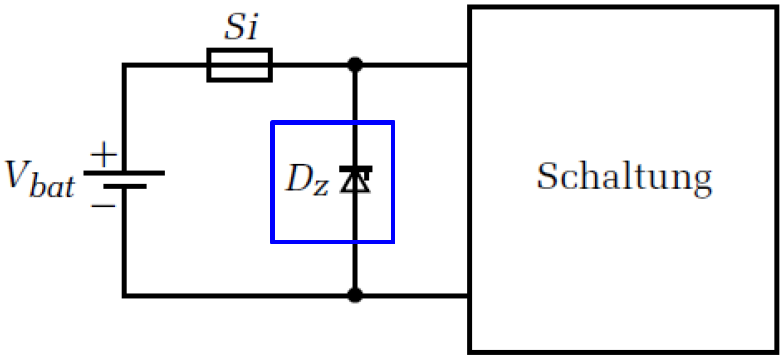
\includegraphics[width=\columnwidth]{images/anwendung_zener_diode.png}
\end{minipage}

\vspace{0.2cm}

\begin{itemize}
    \item \textbf{Anwednung im Durchbruchbereich}
    \item Eingesetzt als Spannungsbegrenzer / Spannungsreferenz \\
        \textrightarrow\ Z-Diode limitiert Spanung am Eingang der Schaltung 
    \item Temperatur-stabilste Referenzspannung $\bm{V_z = 5.6 \, \volt}$
\end{itemize}


\subsubsection{Germanium-Dioden}

\begin{itemize}
    \item Sehr kleine Schwellspannung: $V_D = 0.1 \, \ldots \, 0.4 \, \volt$
    \item Tiefe Temperaturzulässsigkeit: $T_{\rm max} = 75 \, \celsius$ \\
        \textrightarrow\ maximale Stromdichte wesentlich grösser als bei Si-Dioden
\end{itemize}


\subsubsection{Kapazitäts-Diode (Varicap)}

\begin{minipage}[c]{0.45\columnwidth}
    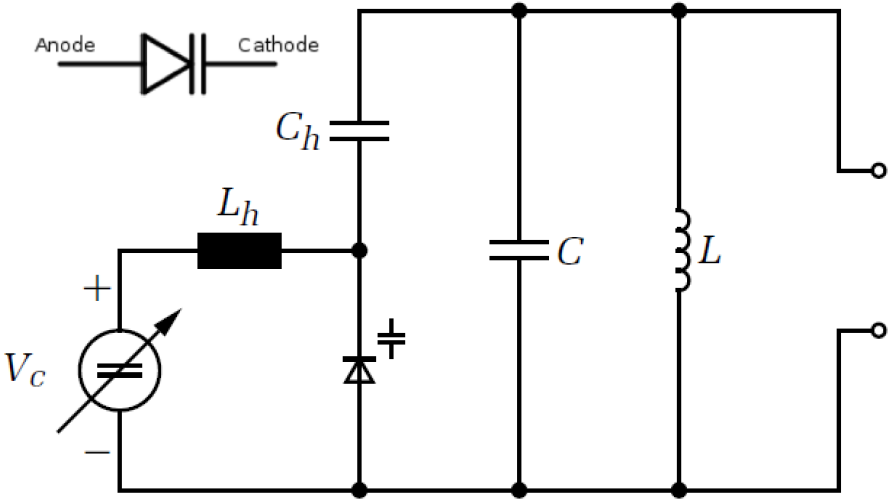
\includegraphics[width=\columnwidth]{images/kapazitaetsdiode.png}
\end{minipage}
\hfill
\begin{minipage}[c]{0.52\columnwidth}
    \raggedright

    \begin{itemize}
        \item Diode mit speziell grosser Kapazität \\
            \textrightarrow\ $C$ sinkt mit steigender Spannung 
        \item Einstellen der Schwingfrequenz in Oszillatoren 
    \end{itemize}
\end{minipage}


		\section{Bipolare Transistoren (BJT)}

\renewcommand{\arraystretch}{1.3}
\begin{tabular}{|ll |ll|}
    \hline
    $I_E$   & Emitter-Strom     & $I_B$             & Basis-Strom                   \\
    \hline
    $I_C$   & Kollektor-Strom   & $\beta = h_{\rm FE}$  & Wechselstrom-Verstärkung  \\
    \hline
\end{tabular}
\renewcommand{\arraystretch}{1}


\subsection{Funktionsweise Bipolarer Transistor}

\begin{minipage}[c]{0.2\columnwidth}
    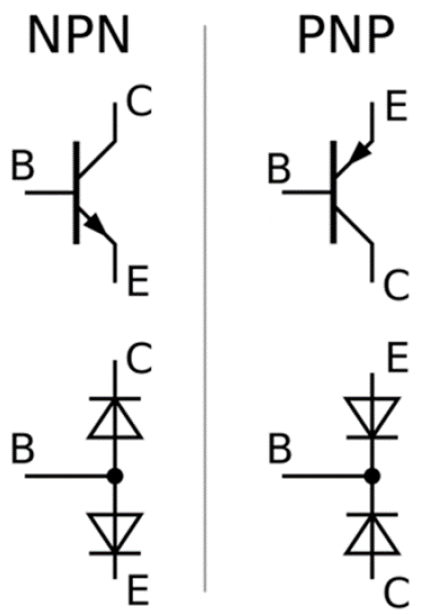
\includegraphics[width=\columnwidth]{images/BJT.png}
\end{minipage}
\hfill
\begin{minipage}[c]{0.78\columnwidth}
    \raggedright

    \begin{itemize}
        \item BK-Diode sperrt im Normalbetrieb
        \item BE-Diode leitet im Normalbetrieb \\
             \textbf{BJT ist nicht symmetrisch!}
        \item Hohe Dotierung im Emitter $(n^+)$
        \item Niedrige Dotierung im Kollektor ($n$, zum Anschluss hin $n^+$) \\
            \textrightarrow\ Kleiner Basis-Strom erzeugt grossen Kollektor-Strom
    \end{itemize}
\end{minipage}


\subsection{Bipolarer Transistor als Stromverstärker}

\begin{minipage}[c]{0.3\columnwidth}
    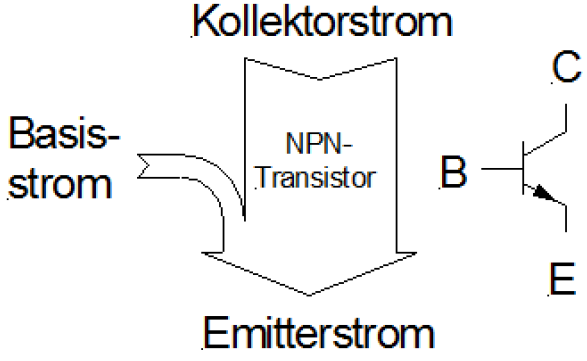
\includegraphics[width=\columnwidth]{images/BJT_funktionsweise.png}
\end{minipage}
\hfill
\begin{minipage}[c]{0.68\columnwidth}
    \renewcommand{\arraystretch}{1.4}
    \begin{tabular}{ll}
        $\boxed{ I_E = I_C + I_B }$         & Stromsummengleichung              \\
        $\boxed{ I_E \approx I_C} $         & vereinfacht für $\beta \gg 1 $    \\
        $\boxed{ I_C = \beta \cdot I_B}$    & 
    \end{tabular}
    \renewcommand{\arraystretch}{1}
\end{minipage}


\subsection{Betriebszustände des Transistors}

\begin{itemize}
    \item \textbf{Normalbetrieb} (forward region): $V_{\rm BE} > 0, \,  V_{BC} < 0$ \\
        E-Diode leitend, C-Diode sperrend. Es gilt: $\bm{I_C= \beta  \cdot I_B}$
    \item \textbf{Sättigung}: $V_{\rm BE} > 0, \,  V_{BC} > 0$ \\
        Beide Dioden leitend. \textbf{Schalter 'ON'}: $V_{\rm CE,sat}$ ca. $0.1..0.3 \, \volt$
    \item \textbf{Sperrbetrieb}: $V_{\rm BE} < 0, \,  V_{BC} < 0$ \\
        Beide Dioden sperrend. \textbf{Schalter 'OFF'}
    \item \textbf{Inversbetrieb}: $V_{\rm BE} < 0, \,  V_{BC} > 0$ \\
        Wie Normalbetrieb, aber nur wenig Stromverstärkung 
\end{itemize}


\subsection{Kennlinien}

\textbf{Im Arbeitsbereich wie Diode: } $ \bm{V_{\rm BE} = 0.7 \, \volt}$

\vspace{0.2cm}

\begin{minipage}[c]{0.33\columnwidth}
    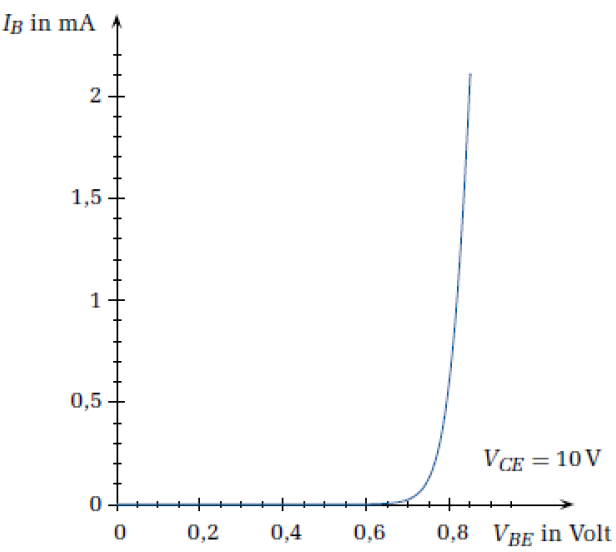
\includegraphics[width=\columnwidth]{images/BJT_eingangskennlinie.png}
\end{minipage}
\hfill
\begin{minipage}[c]{0.55\columnwidth}
    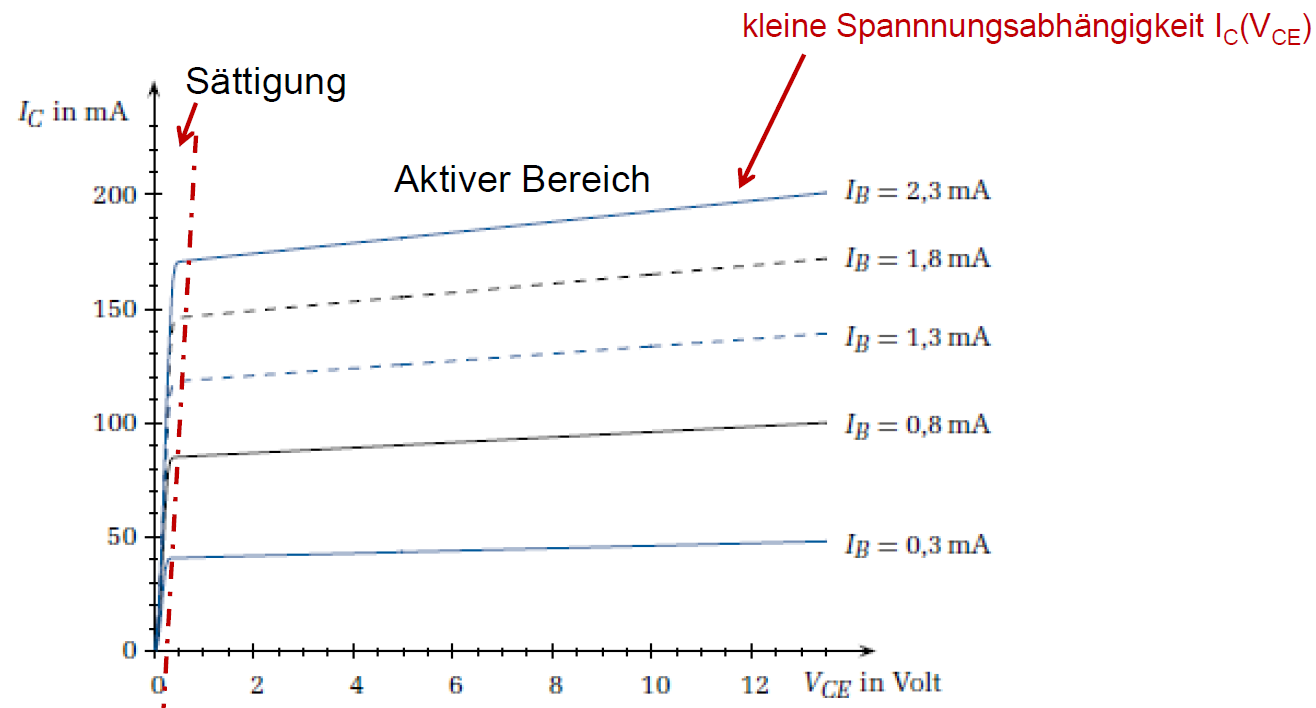
\includegraphics[width=\columnwidth]{images/BJT_ausgangskennlinien.png}
\end{minipage}


\subsection{Verlustleistung und Erwärmung im Transistor}

\vspace{-0.2cm}

$$ \boxed{ P_v = V_{\rm CE} \cdot (I_B + I_C) \approx  V_{\rm CE} \cdot I_C = V_{\rm AP} \cdot I_C } $$
$$ \boxed{ \Delta T = R_{\rm th} \cdot P_v }$$



\subsection{Ersatzschlatungen von Transistoren}

\subsubsection{Grosssignal-Ersatzschaltung}

\begin{minipage}[c]{0.48\columnwidth}
    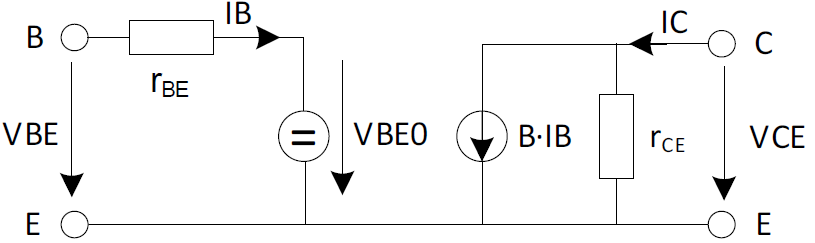
\includegraphics[width=\columnwidth]{images/BJT_grosssignalersatzschaltung.png}
\end{minipage}
\hfill
\begin{minipage}[c]{0.48\columnwidth}
    $$ \boxed{ R_{\rm BE} = \frac{n \cdot V_T}{I_{\rm B0}} } \qquad \boxed{ r_{\rm CE} \approx \frac{V_A}{I_C}} $$
\end{minipage}


\subsubsection{Kleinsignal-Ersatzschaltungen}

\begin{minipage}[c]{0.45\columnwidth}
    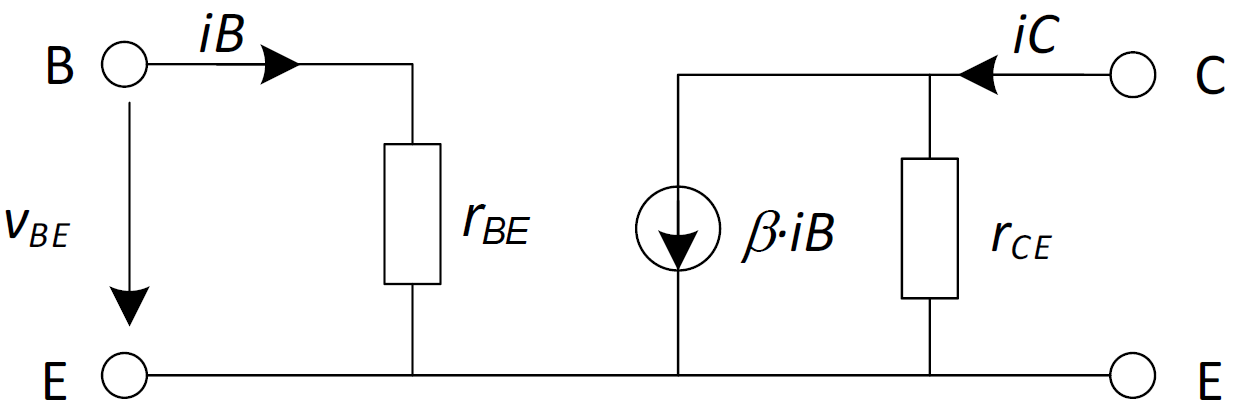
\includegraphics[width=\columnwidth]{images/BJT_kleinsignalmodell_1.png}
\end{minipage}
\hfill
\begin{minipage}[c]{0.45\columnwidth}
    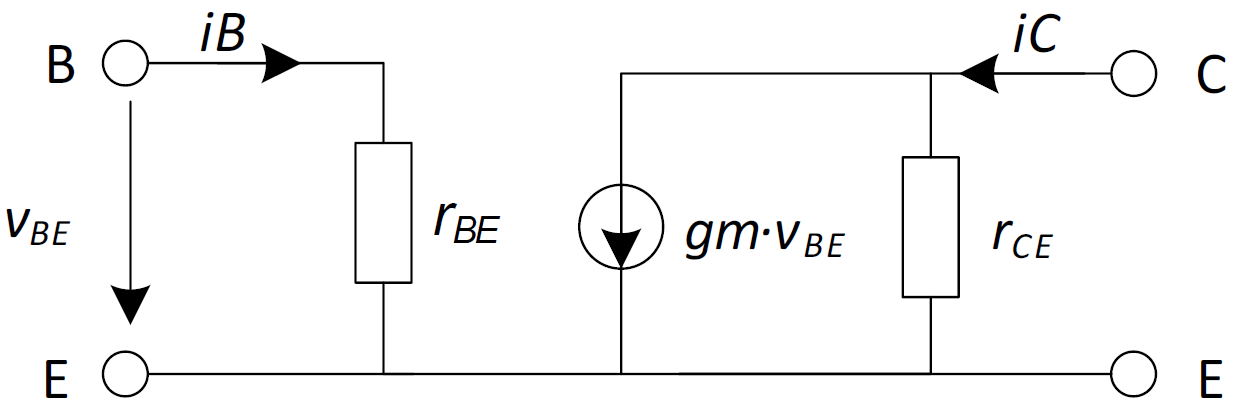
\includegraphics[width=\columnwidth]{images/BJT_kleinsignalmodell_2.png}
\end{minipage}

\vspace{0.2cm}

\begin{tabular}{@{}ccc@{}}
    $\boxed{ r_{\rm BE} = \frac{n \cdot V_T}{I_{\rm B0}} }$ & $\boxed{ gm = \frac{\beta}{r_{\rm BE}} = \frac{I_C}{n \cdot V_T} }$ & $\boxed{ r_{\rm CE} \approx \frac{V_A}{I_C} = \frac{200 \, \volt}{I_C} } \; V_A: \text{Early Spannung}$
\end{tabular}


\subsection{Emitterschaltung}

\begin{minipage}[c]{0.3\columnwidth}
    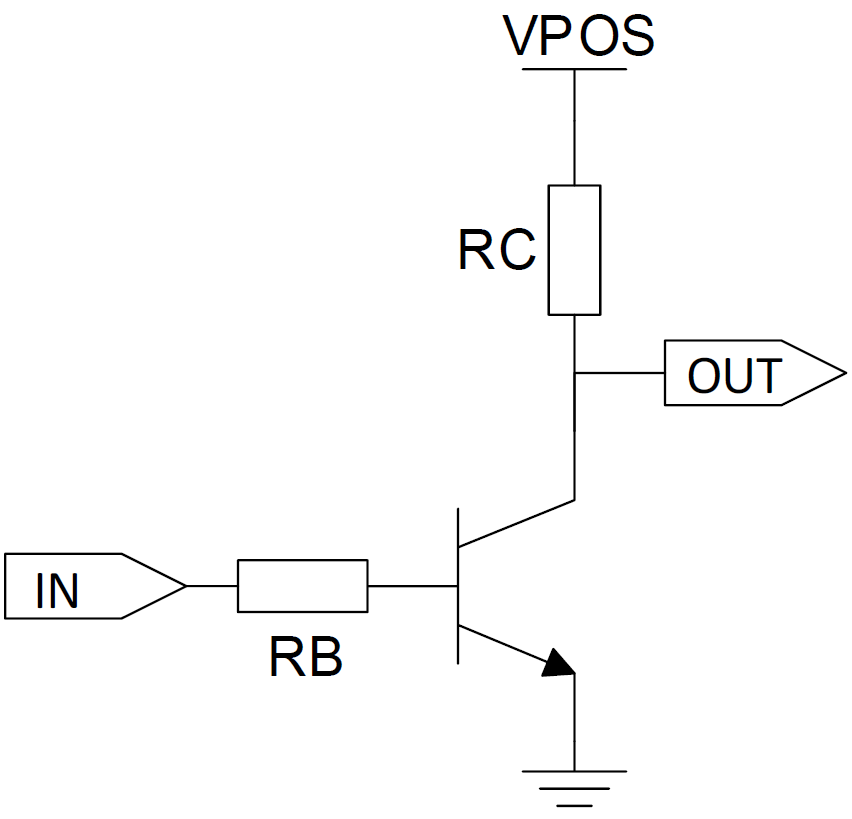
\includegraphics[width=0.8\columnwidth]{images/emitterschaltung_2.png}
    $$ \boxed{I_{\rm RC} = \frac{(V_{\rm POS} - V_{\rm out})}{R_C} } $$
\end{minipage}
\hfill
\begin{minipage}[c]{0.55\columnwidth}
    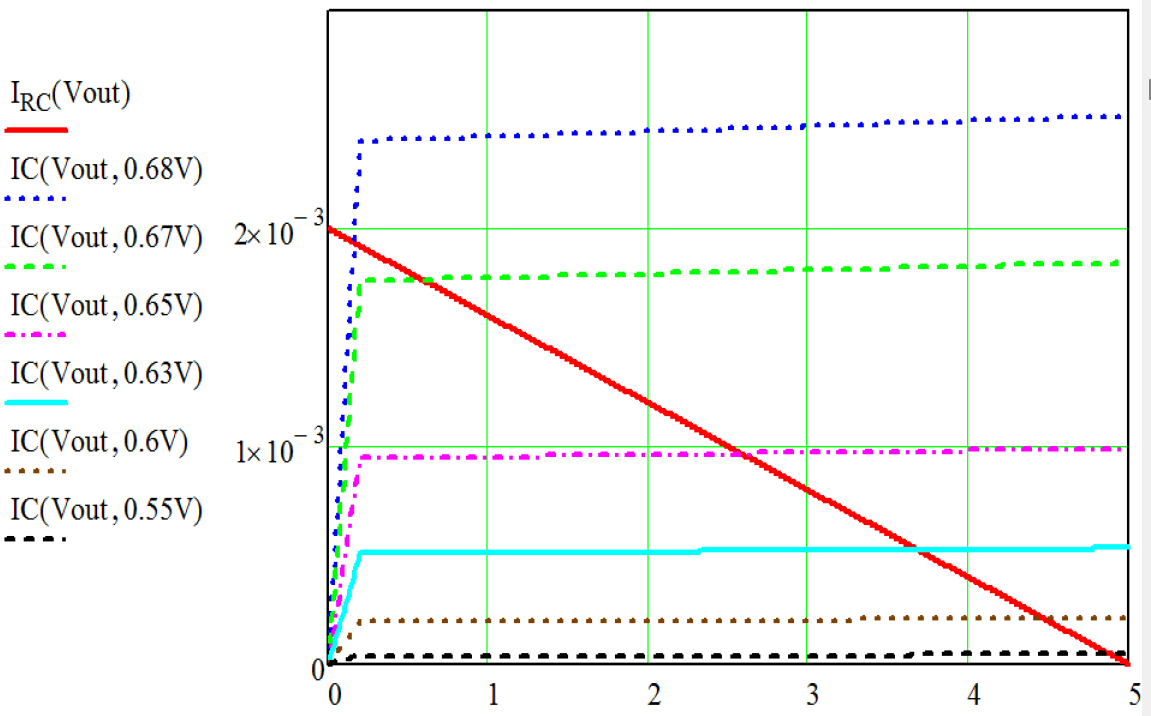
\includegraphics[width=\columnwidth]{images/emitterschaltung_kennlinienfeld.png}
\end{minipage}

\vspace{0.2cm}

\myul{\textbf{Arbeitsbereiche}}

\vspace{0.1cm}

\begin{tabular}{lll}
    Sperrend        & $ 0 \, \volt < V_{\rm BE} < ~0.6 \, \volt$ & $V_{\rm out} = V_{\rm POS}$                          \\
    Verstärkend     & $ \approx 0.6 \, \volt < V_{\rm BE} < ~0.8 \, \volt$ & $V_{\rm out}$ sinkt auf $V_{\rm CE,sat}$   \\
    Durchgesteuert  & $ \approx 0.8 \, \volt < V_{\rm BE}$ & $V_{\rm out} = V_{\rm CE,sat} $ 
\end{tabular}


\subsubsection{Emitterschaltung berechnen}

Gültig für $V_{\rm CE,sat} < V_{\rm out} < V_{\rm POS}$

\begin{minipage}[c]{0.7\columnwidth}
    $$ \boxed{ I_{\rm RC} = \frac{(V_{\rm POS} - V_{\rm out})}{R_C} = I_C = \beta \cdot I_S \cdot e^{\frac{V_{\rm in}}{n \cdot V_T}} } $$
    $$ \boxed{ V_{\rm out} = V_{\rm POS} - R_C \cdot \beta \cdot I_S \cdot e^{\frac{V_{\rm in}}{n \cdot V_T}} } $$
\end{minipage}
\begin{minipage}[c]{0.25\columnwidth}
    \[ \boxed{A = \frac{-R_c I_c}{n V_t}}\]
\end{minipage}

$V_{\rm out} = f(V_{\rm in})$ Exponentialfunktion: Start @ $V_{\rm POS}$, Ende @ $V_{\rm CE,sat}$


\subsection{Transistorverstärker mit Arbeitspunkteinstellung}

Spannung $V_{\rm out}$ soll auf $V_{AP}$ eingestellt werden: \\
$V_B$ entspricht Diodenspannung $\bm{ V_B = 0.7 \, V} $ 


\subsubsection{AP über Strom (bzw. $\bm{R_1}$) einstellen}

\begin{minipage}[c]{0.3\columnwidth}
    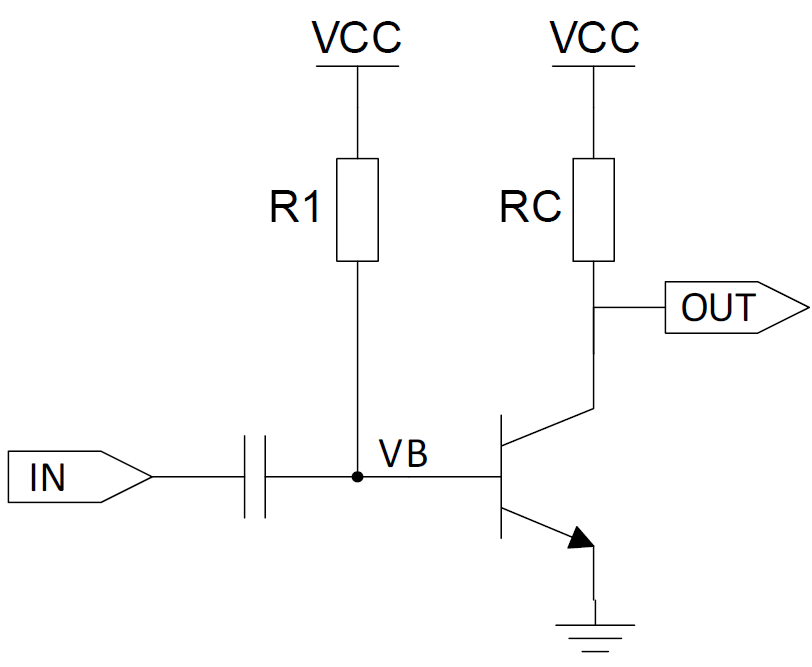
\includegraphics[width=\columnwidth]{images/emitterschaltung_AP_1.png}
\end{minipage}
\hfill
\begin{minipage}[c]{0.69\columnwidth}
    $$ \boxed{ I_{\rm C0} = \frac{V_{AP}}{R_C} } \quad \boxed{ I_{B0} = \frac{I_{\rm C0}}{\beta} } \quad \boxed{ R_1 = \frac{V_{CC} - V_B}{I_{B0}} } $$
\end{minipage}


\subsubsection{AP über Spannung (bzw. $\bm{R_1}$ und $\bm{R_2}$) einstellen}
\label{AP über Spannung (bzw. $R_1$ und $R_2$) einstellen}

\begin{minipage}[c]{0.3\columnwidth}
    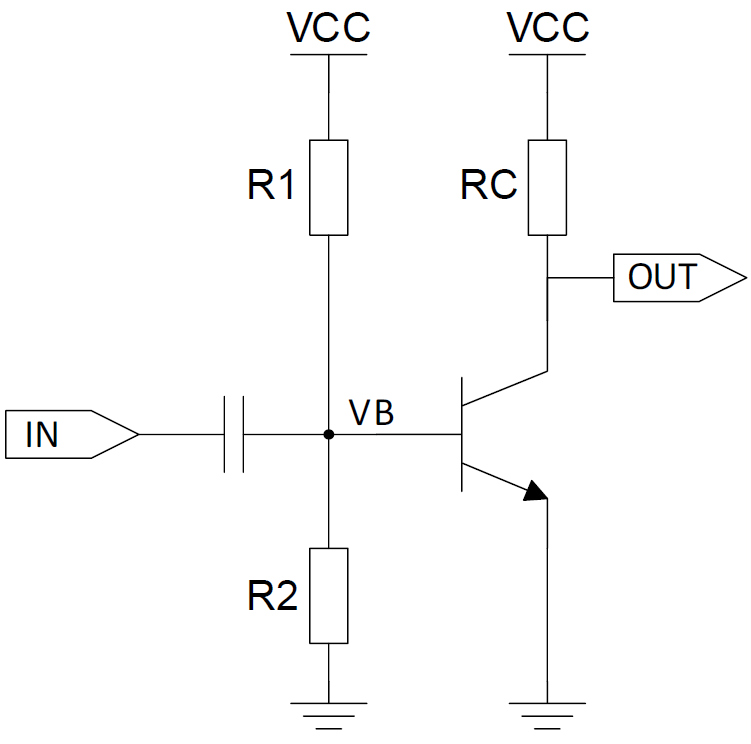
\includegraphics[width=\columnwidth]{images/emitterschaltung_AP_2.png}
\end{minipage}
\hfill
\begin{minipage}[c]{0.69\columnwidth}
    $$ \boxed{ I_{\rm C0} = \frac{V_{\rm AP}}{R_C} } \quad \boxed{ I_{\rm B0} = \frac{I_{\rm C0}}{\beta} } \quad \boxed{ I_{\rm R2} \geq 10 \cdot I_{\rm B0} } $$
    $$ \boxed{ R_2 = \frac{V_B}{I_{\rm R2}} } \quad \boxed{ R_1 = \frac{(V_{\rm CC} - V_B)}{I_{\rm B0} + I_{\rm R2}} } $$
\end{minipage}

\textrightarrow\ Schaltung hat sehr grosse Toleranzen! \\
\textrightarrow\ Temperatur-Abhägigkeit von $V_{\rm BE} = -2 \, \frac{\milli \volt}{\kelvin}$ \textrightarrow\ Faktor 2 alle $10 \, \celsius$ \\
\textrightarrow\ Somit ändern sich auch $I_B$ bzw. $I_C$ alle $10 \, \celsius$


\subsubsection{Transistorverstärker mit Stromgegenkopplung}

\begin{minipage}[c]{0.27\columnwidth}
    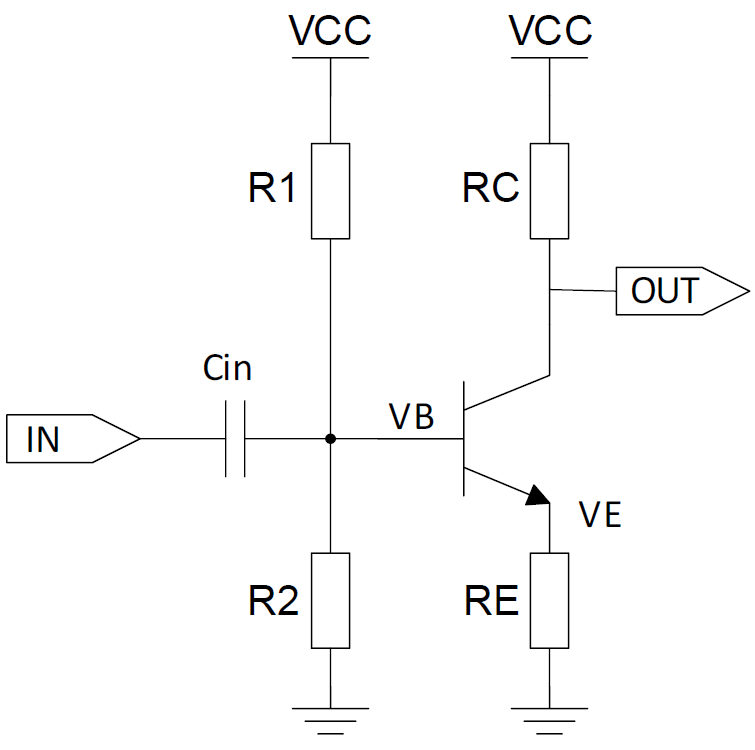
\includegraphics[width=\columnwidth]{images/transistorverstaerker_stromgegenkopplung.png}
\end{minipage}
\hfill
\begin{minipage}[c]{0.66\columnwidth}
    \raggedright
    \myul{\textbf{Reduktion der Toleranzen}}

    \vspace{0.1cm}

    $V_{\rm BE}$ entspricht Diodenspannung $\bm{ V_B = 0.7 \, V} $

    \vspace{0.2cm}
    $V_{\rm in}$ \textbf{steigt} um $\Delta V$ \\
    \textrightarrow\ Dann steigt auch $V_B$ um $\Delta V$ \\
    \textrightarrow\ Dann steigt auch $V_E$ um $\Delta V$
\end{minipage}

\vspace{0.2cm}

\renewcommand{\arraystretch}{1.2}
\begin{tabular}{ll}
    Strom in $R_E$ steigt:                      & $\Delta I_{\rm RE} = \frac{\Delta V_E}{R_E} \approx \frac{\Delta V_{\rm in}}{R_E}$    \\
    Strom in $R_C$ steigt:                      & $\Delta I_{\rm RC} = \frac{\Delta V_E}{R_E} \approx \frac{\Delta V_{\rm in}}{R_E}$    \\
    Spannung an $V_{\rm out}$ \textbf{sinkt}:   & $\Delta V_{\rm out} \approx - \frac{R_C}{R_E} \cdot \Delta V_{\rm in}$
\end{tabular}
\renewcommand{\arraystretch}{1}


\subsubsection{Transistorverstärker mit Stromgegenkopplung \& Kondi}

\begin{minipage}[c]{0.27\columnwidth}
    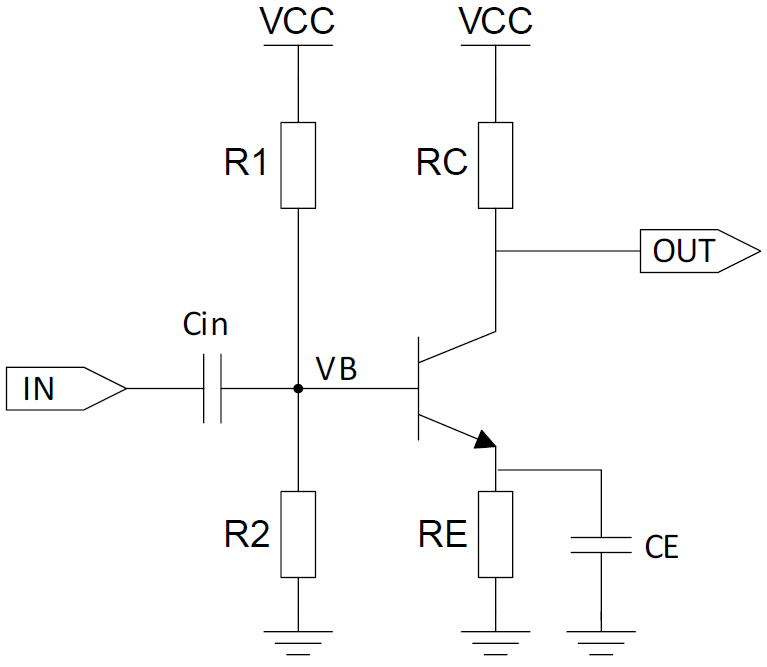
\includegraphics[width=\columnwidth]{images/transistorverstaerker_stromgegenkopplung_kondensator.png}
\end{minipage}
\hfill
\begin{minipage}[c]{0.66\columnwidth}
    $C_E$ schliesst $R_E$ für hohe Frequenzen kurz \\
    Somit wird der AP 'stabil' mit Widerständen eingestellt

    \vspace{0.2cm}

    Berechnung der Schaltung siehe Abschnitt \ref{AP über Spannung (bzw. $R_1$ und $R_2$) einstellen}
\end{minipage}


\subsection{Transistor als Schalter}

\begin{minipage}[c]{0.3\columnwidth}
    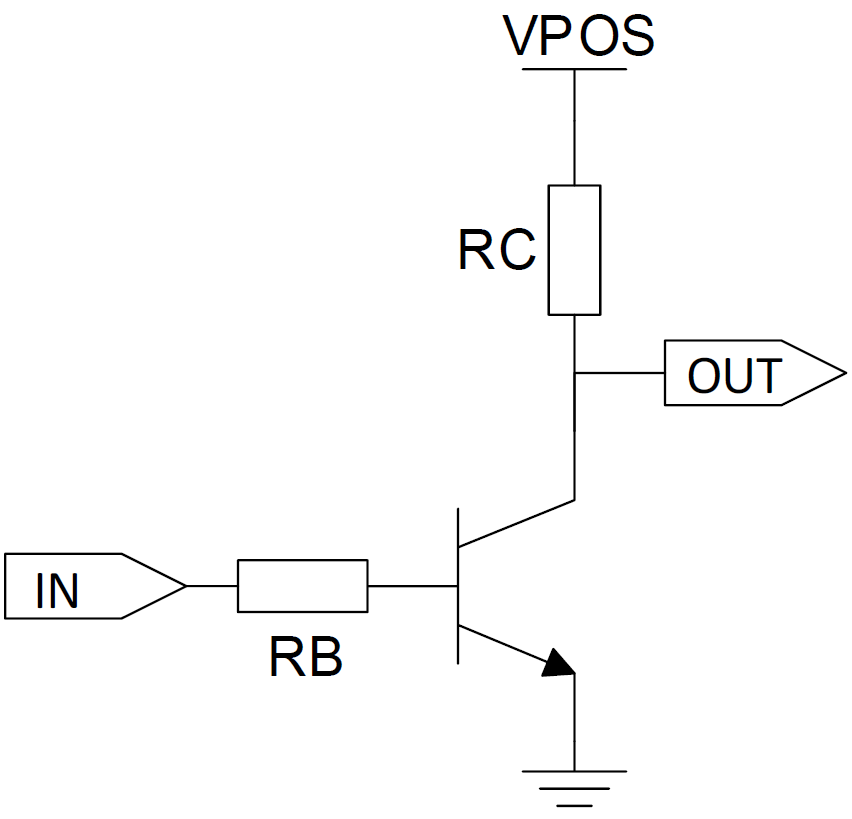
\includegraphics[width=\columnwidth]{images/emitterschaltung_2.png}
\end{minipage}
\hfill
\begin{minipage}[c]{0.46\columnwidth}
    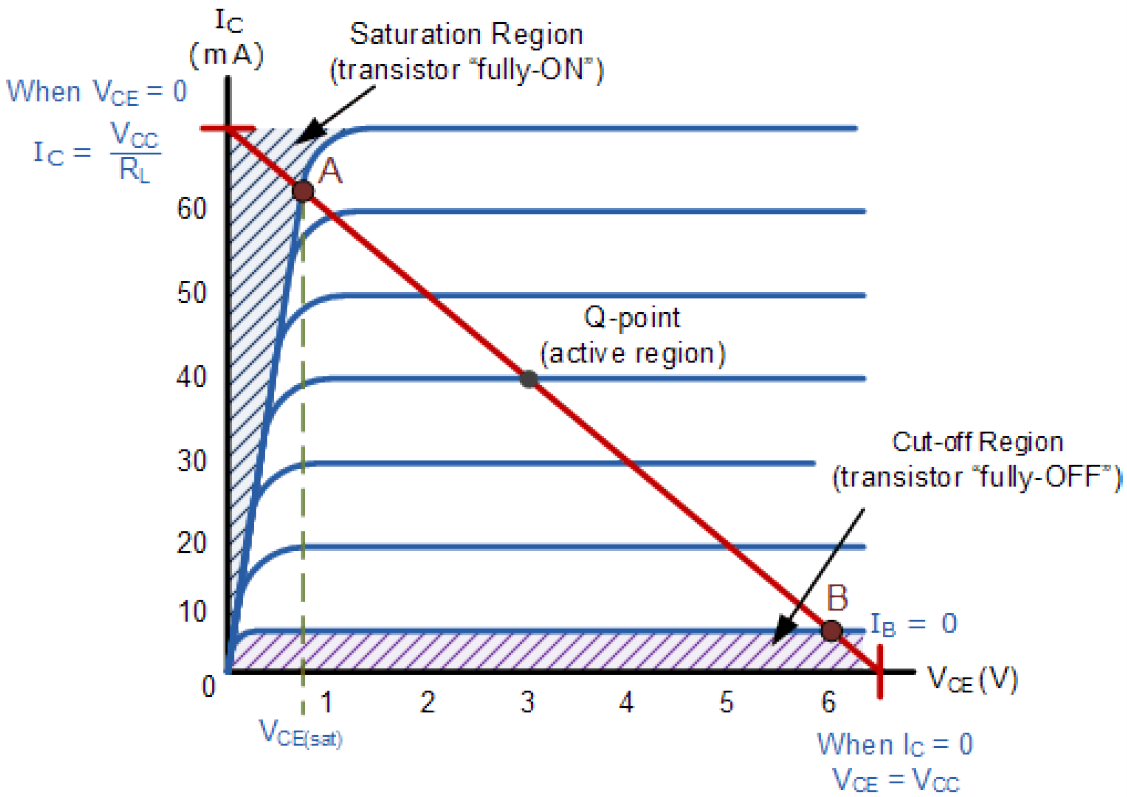
\includegraphics[width=\columnwidth]{images/transistor_als_schalter.png}
\end{minipage}

\vspace{0.2cm}

\begin{tabular}{lll}
    ON (A)  & $V_{\rm in} > 0.6$, grosses $I_B$ & \textrightarrow\ $V_{\rm out} = V_{\rm CE, sat}$  \\
    OFF (B) & $V_{\rm in} < 0.6 \, V$, $I_B = 0$ &  \textrightarrow\ $V_{\rm out} = V_{\rm CC}$
\end{tabular}


\subsection{Basisschaltung}

\subsubsection{Basischaltung als Verstärkerschaltung}

\begin{minipage}[c]{0.35\columnwidth}
$\bm{ V_{\rm BE0} = 0.7 \, V} $

\vspace{0.2cm}

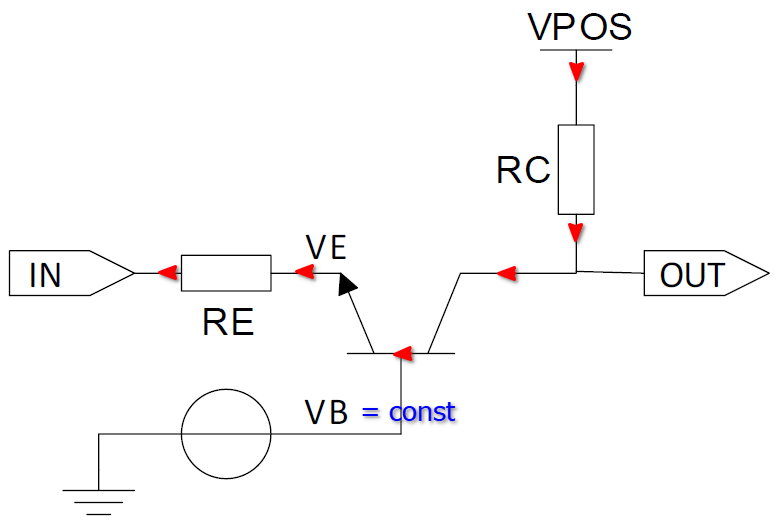
\includegraphics[width=\columnwidth]{images/basisschaltung_2}
\end{minipage}
\hfill
\begin{minipage}[c]{0.62\columnwidth}
    $$ \boxed{ I_E = I_C = \frac{(V_{\rm in} - V_{\rm BE0})}{R_E}  }$$
    $$ \boxed{ V_{\rm out} = V_{\rm POS} - I_E \cdot R_C - V_B}$$
    $$ \boxed{ \frac{\Delta V_{\rm out}}{\Delta V_{\rm in}} = \frac{R_C}{R_E} } \quad \boxed{ \Delta I = \frac{\Delta V_{\rm in}}{R_E}} $$
\end{minipage}

\vspace{0.2cm}

\myul{\textbf{Voraussetzungen:}}

\vspace{0.1cm}

\begin{tabular}{ll}
    $V_{\rm in} < V_B - V_{\rm BE0}$        & Strom fliesst aus Emitter     \\
    $V_{\rm out} > V_E + V_{\rm CE,sat}$    &                               \\
    $ V_B - V_{\rm BE0} + V_{\rm CE,sat}$   & Transtor als Verstärker       \\
    $I_B \approx 0$                         & \textrightarrow\ $I_E = I_C$
\end{tabular}


\subsubsection{Summierung von Bias- und Signalspannung}

\begin{minipage}[c]{0.35\columnwidth}
    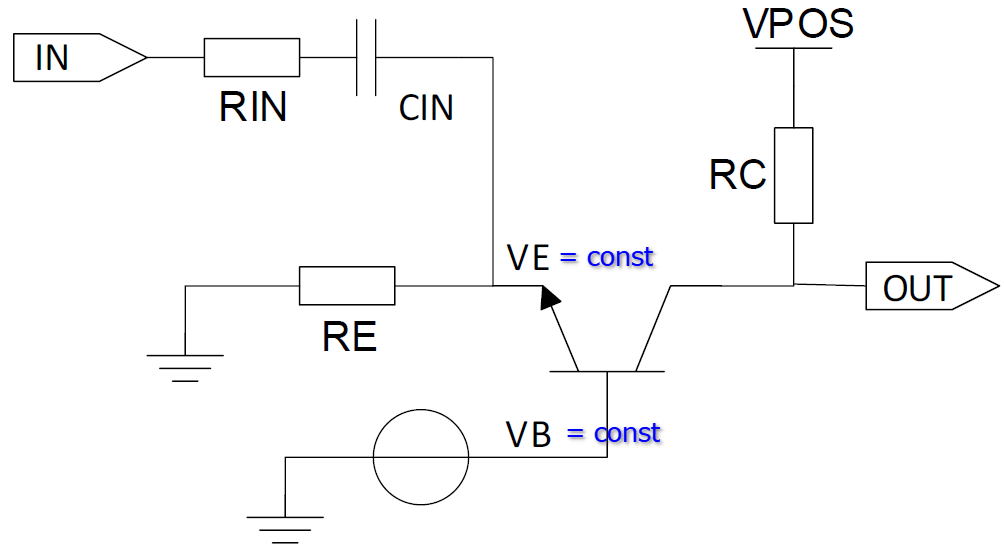
\includegraphics[width=\columnwidth]{images/basisschaltung_summierung.png}
\end{minipage}
\hfill
\begin{minipage}[c]{0.62\columnwidth}
    $\bm{ V_{\rm BE0} = 0.7 \, V} $

    $$ \boxed{ \Delta I_{\rm in} = \frac{\Delta V_{\rm in}}{R_{\rm in}} } \quad \boxed{ V_E = V_B - V_{\rm BE0} } $$
\end{minipage}

$$ \boxed{ V_{\rm out} = V_{\rm POS} - \Bigg( \frac{V_E}{R_E} - \frac{\Delta V_{\rm in}}{R_{\rm in}} \Bigg) \cdot R_C = V_{\rm out0} + \Delta V_{\rm in} \cdot \frac{R_C}{R_{\rm in}} } $$ 


\subsection{Kollektorschaltung (Emitterfolger)}

\begin{minipage}[c]{0.27\columnwidth}
    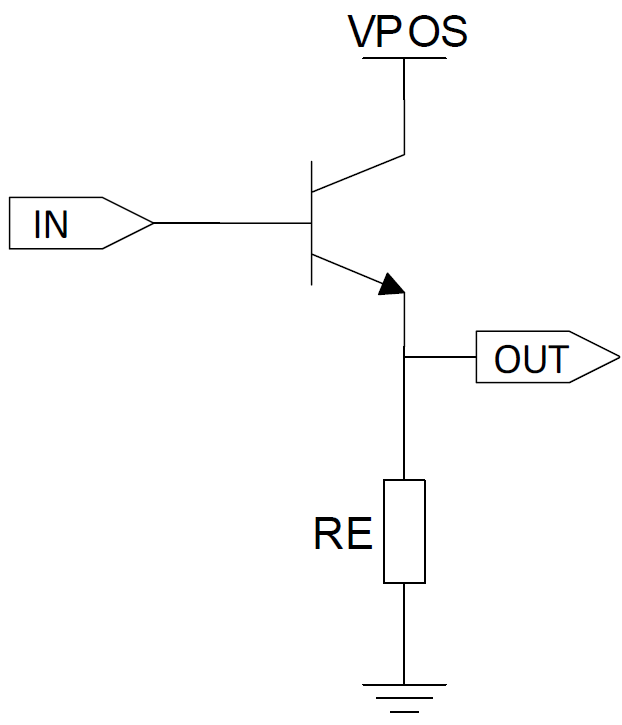
\includegraphics[width=\columnwidth]{images/kollektorschaltung_2.png}
\end{minipage}
\hfill
\begin{minipage}[c]{0.68\columnwidth}
    $$ \boxed{V_{\rm out} = V_{\rm in} - V_{\rm BE0} } $$
    $$ \boxed{ \text{Spannungsverstärkung } \approx 1 } $$

    \begin{itemize}
        \item Hoher Eingangswiderstand \\
            \textrightarrow\ $V_{\rm in}$ kaum belastet
        \item Tiefer Ausgangswiderstand \\
            \textrightarrow\ $V_{\rm out}$ kann Strom liefern 
    \end{itemize}
\end{minipage}


\subsection{Übresicht Verstärkertypen}

\begin{minipage}[c]{0.48\columnwidth}
    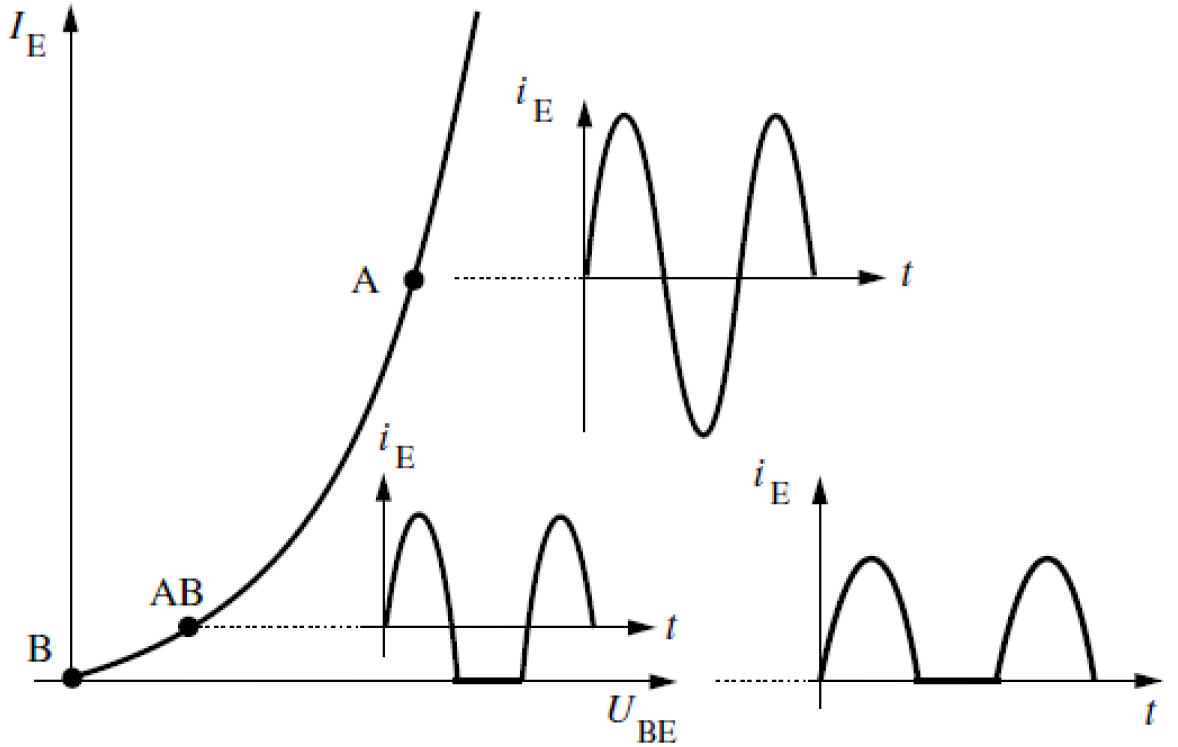
\includegraphics[width=\columnwidth]{images/verstaerker_uebersicht.png}
\end{minipage}
\hfill
\begin{minipage}[c]{0.48\columnwidth}
    \begin{tabular}{ll}
        A   & Einfacher Emitterfolger           \\
            & \textrightarrow\ sehr ineffizient \\
            & ($\eta_{\rm max} = 25$ \%)        \\
        B   & Effizient, aber verzerrt          \\
            & Signale um $0 \, V$               \\
            & ($\eta_{\rm max} = 78.5$ \%)      \\
        AB  & Guter Kompromiss für              \\
            & viele Anwendungen 
    \end{tabular}
\end{minipage}


\subsection{Class-A Verstärker}

\begin{minipage}[c]{0.3\columnwidth}
    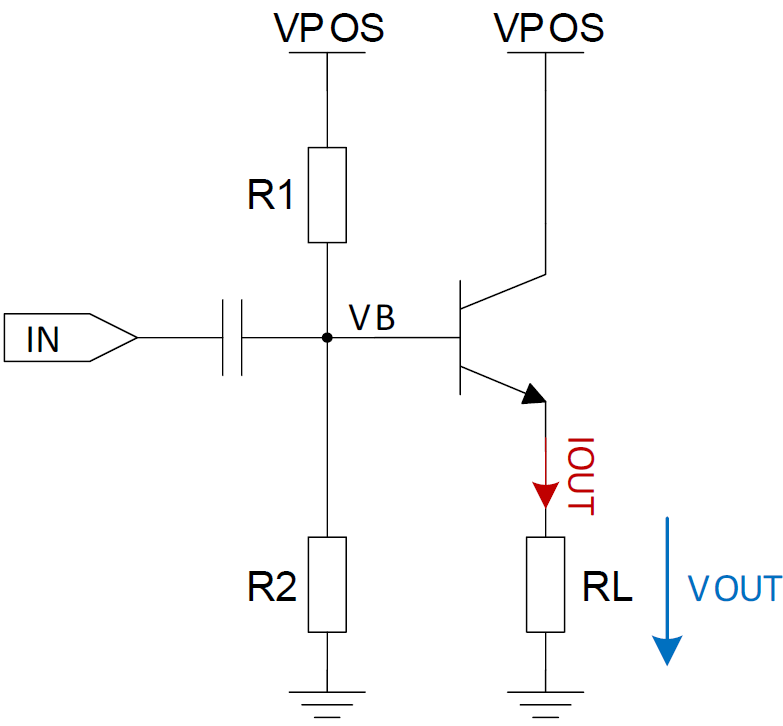
\includegraphics[width=\columnwidth]{images/class-A_verstaerker.png} 
\end{minipage}
\hfill
\begin{minipage}[c]{0.68\columnwidth}
    \raggedright
    $\bm{ V_{\rm BE0} = 0.7 \, V} $

    \vspace{0.2cm}

    \begin{itemize}
        \item $V_B$ eingestellt mit $R_1$ und $R_2$
        \item $V_B$ Es fliesst immer Strom durch $R_L$ \\
            \textrightarrow\ höheres $V_B$ \textrightarrow\ grösserer DC-Strom \\
            \textrightarrow\ grössere Verlustleistung
        \item wenn nicht 100\% ausgesteuert wird, nimt der Wirkungsgrad im Quadrat ab
    \end{itemize}
\end{minipage}


\subsubsection{Wirkungsgrad des Class-A Verstärkers}

$$ \boxed{ \eta \approx \frac{P_{\rm AC}}{P_{\rm DC} } \approx 25\%_{\text{MAX}}} \quad 
\boxed{P_{\rm AC} = V_{\rm eff} \cdot I_{\rm eff} = \frac{\hat{V}^2}{2 \cdot R_L}} \quad
\boxed{P_{\rm AC,MAX} =\frac{V_{\rm max}}{\sqrt{2}} \frac{\hat{I}_{\rm max}}{\sqrt{2}} = \frac{V_{\rm POS}^2}{8 R_L} } $$
$$ \boxed{ P_{\rm DC} = V_{\rm POS} \cdot I_L = V_{\rm POS} \cdot \frac{V_{\rm POS}}{2 \cdot R_L} = \frac{V_{\rm POS}^2}{2 \cdot R_L} } $$


\subsection{Class-B Verstärker}

\begin{minipage}[c]{0.3\columnwidth}
    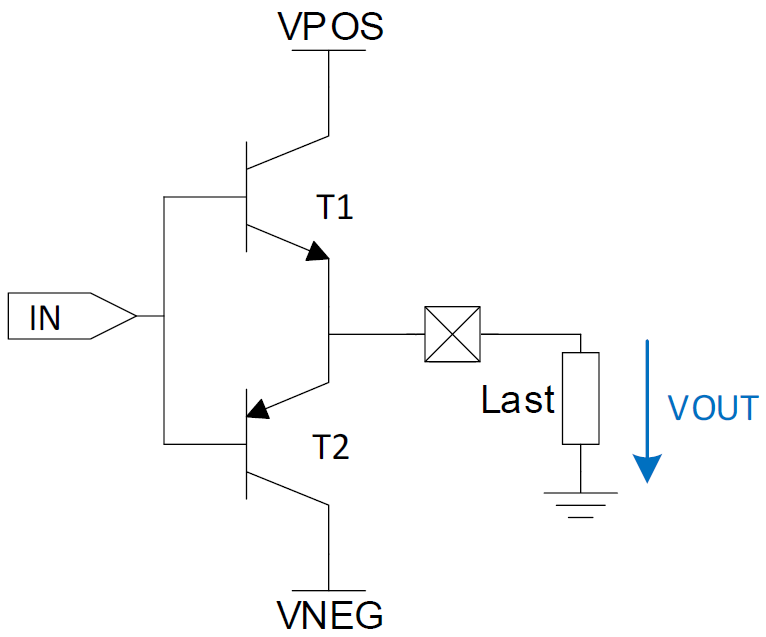
\includegraphics[width=\columnwidth]{images/class-B_verstaerker.png} 
\end{minipage}
\hfill
\begin{minipage}[c]{0.68\columnwidth}
    \raggedright

    \begin{itemize}
        \item $T1$ leitet für pos. Spannungen
        \item $T2$ leitet für neg. Spannungen \\
            \textrightarrow\ Es leiten nie beide Transistoren!
        \item Für $-0.7 \, V < V_{\rm in} < 0.7 \, V$ sperren beide Transistoren \\
            \textrightarrow\ \textbf{Verzerrungen} um $0 \, \volt$ 
    \end{itemize}
\end{minipage}


\subsubsection{Wirkungsgrad des Class-B Verstärkers}

\vspace{-0.2cm}

$$ \boxed{ \eta \approx \frac{P_{\rm AC}}{P_{\rm DC}} } \quad \boxed{ P_{\rm AC} = V_{\rm eff} \cdot I_{\rm eff} = \frac{\hat{V}^2}{2 \cdot R_L} } (\hat{V} \Rightarrow {\rm Spitzenwert})$$
$$ \boxed{ P_{\rm DC} = \frac{2}{T} \int\limits_0^{\frac{T}{2}}  V_{\rm POS} \cdot i(t) \, \diff t =
    \frac{2}{T} \int\limits_0^{\frac{T}{2}}  V_{\rm POS} \cdot \frac{V_{\rm max}}{R_L} \sin(x) \, \diff x = \frac{2}{\pi} \frac{V_{\rm POS} \cdot V_{\rm max}}{R_L} } $$


\subsection{Class-AB Verstärker}

\begin{minipage}[c]{0.3\columnwidth}
    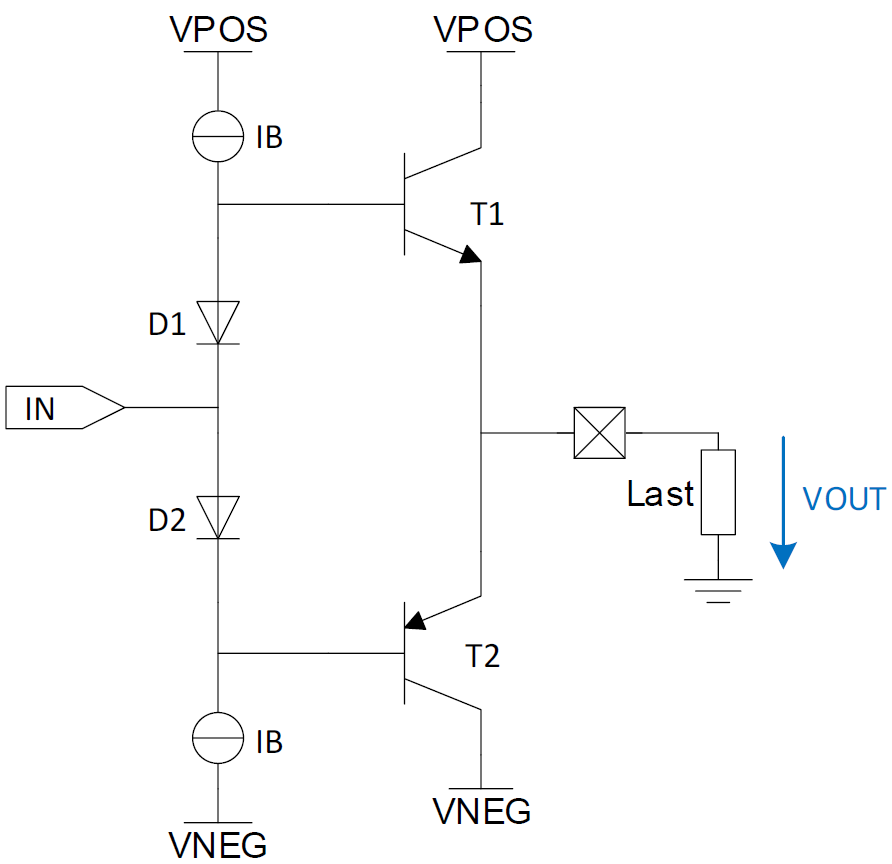
\includegraphics[width=\columnwidth]{images/class-AB_verstaerker.png} 
\end{minipage}
\hfill
\begin{minipage}[c]{0.68\columnwidth}
    \raggedright
    $\bm{ V_{\rm BE0} = 0.7 \, \volt} $

    \vspace{0.2cm}

    \begin{itemize}
        \item $D_1$: $T_1$ leitet für $V_{\rm in} > 0 \, \volt$
        \item $D_2$: $T_2$ leitet für $V_{\rm in} < 0 \, \volt$
        \item Einer der Transistoren leitet immer \\
            \textrightarrow\ Im Übergangsbereich leiten beide wenig
        \item $I_B$ liefern Basis- und Diodenströme 
    \end{itemize}
\end{minipage}


\subsubsection{Bipolar-Transistor mit $\bm{V_{\rm BE} = V_{\rm CE}}$}

\begin{minipage}[c]{0.2\columnwidth}
    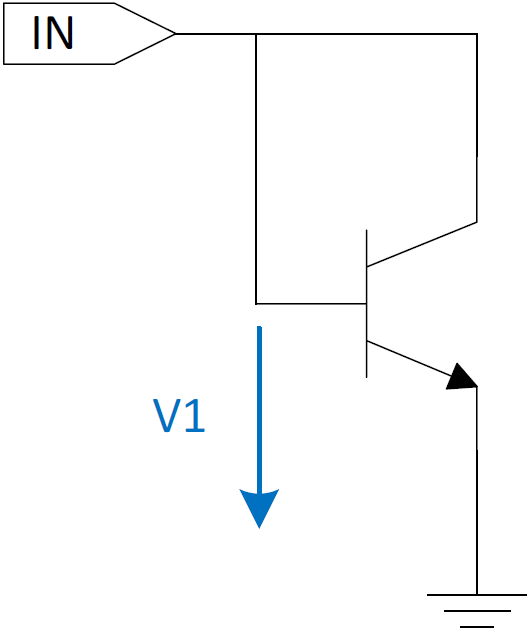
\includegraphics[width=\columnwidth]{images/BJT_VBE_VCE.png}
\end{minipage}
\hfill
\begin{minipage}[c]{0.2\columnwidth}
    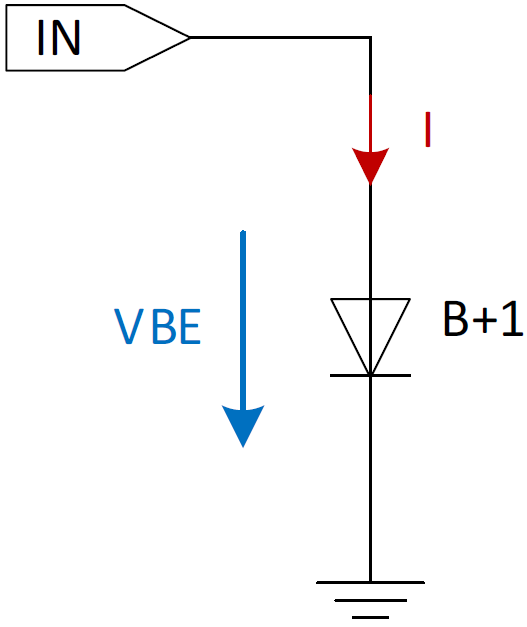
\includegraphics[width=\columnwidth]{images/BJT_parallele_dioden.png}
\end{minipage}
\hfill
\begin{minipage}[c]{0.2\columnwidth}
    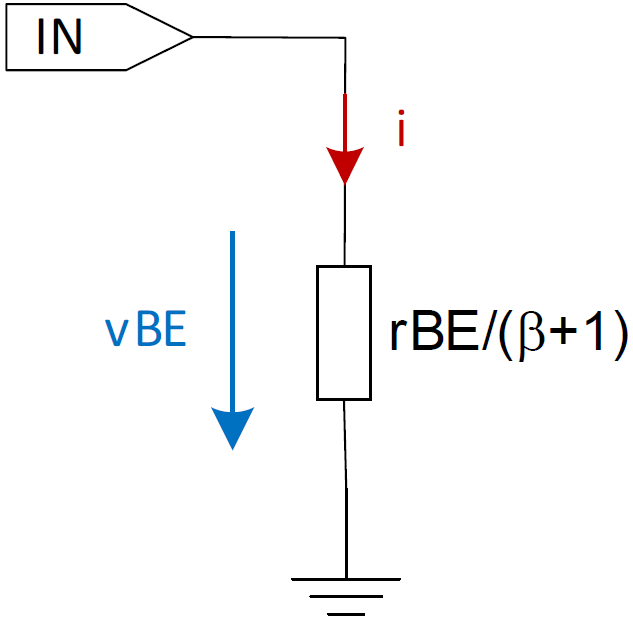
\includegraphics[width=\columnwidth]{images/BJT_kleinsignalersatzschaltung.png}
\end{minipage}
\hfill
\begin{minipage}[c]{0.3\columnwidth}
    $$ \boxed{r_{\rm BE} = \frac{n \cdot V_T}{I_{\rm B0}} } $$
    $$ \boxed{r_{\rm d,eq} = \frac{n \cdot V_T}{I_{\rm C0}} } $$
\end{minipage}


\subsection{Stromspiegel}

\begin{minipage}[c]{0.35\columnwidth}
    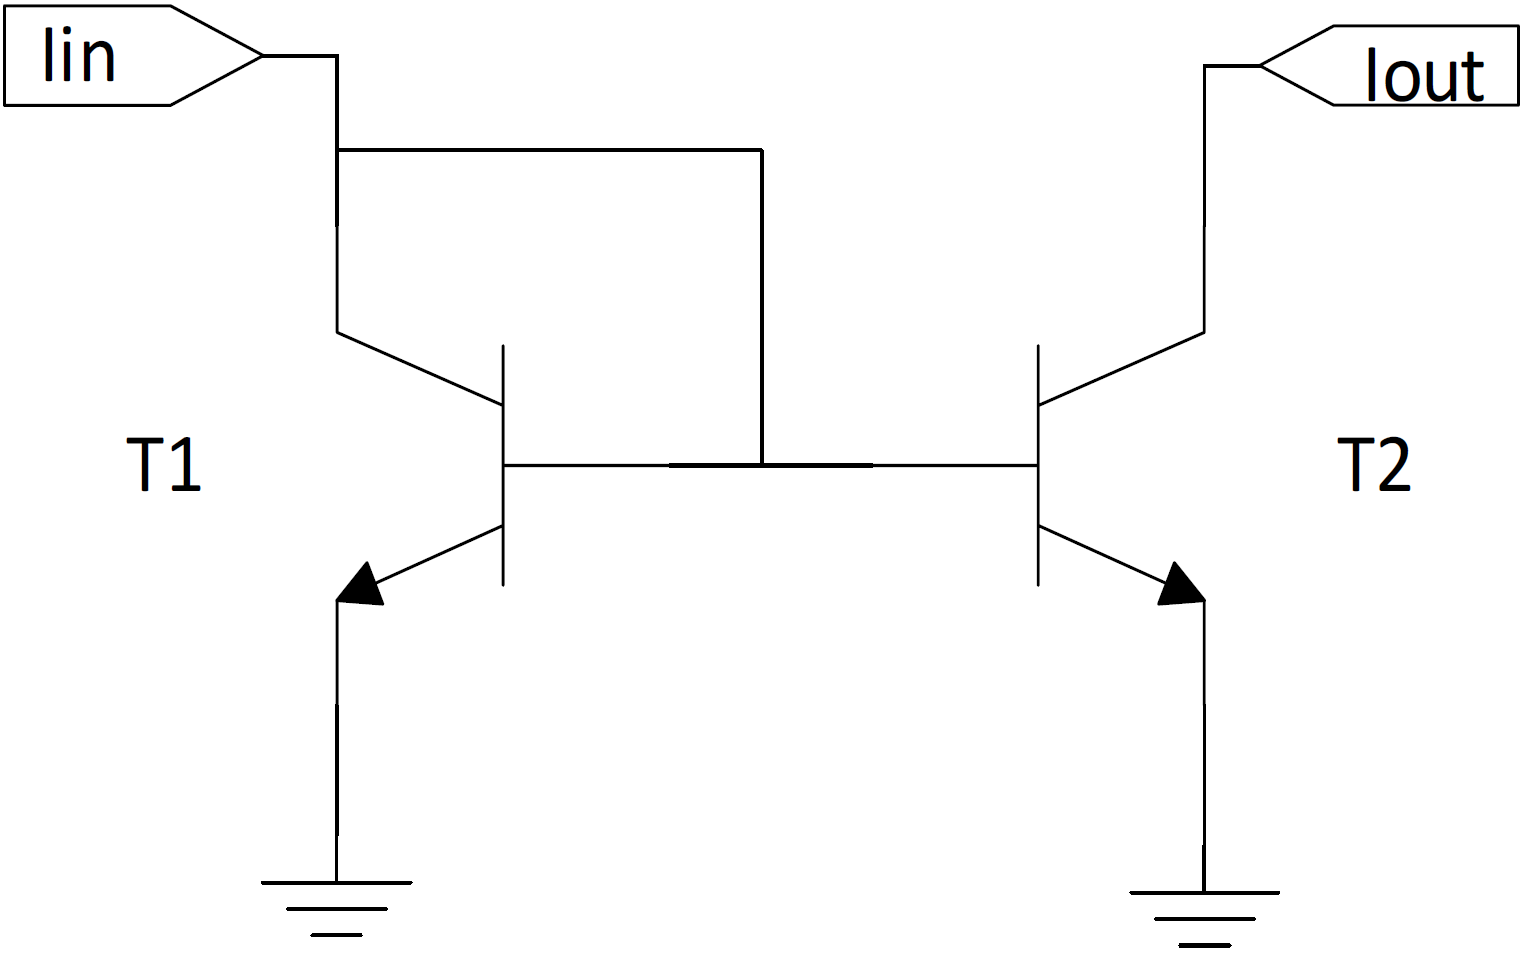
\includegraphics[width=\columnwidth]{images/stromspiegel.png}
\end{minipage}
\hfill
\begin{minipage}[c]{0.63\columnwidth}
    \begin{center}
        \begin{itemize}
            \item $T_1$ als Diode geschaltet
            \item $T_2$ hat gleiches $V_{\rm BE}$
            \item $V_{\rm BE,1} = V_{BE,2}$ \textrightarrow\ $I_{\rm B1} = I_{\rm B2}$ \\
                \textrightarrow\ $I_{\rm C1} = I_{\rm C2}$ 
        \end{itemize}
    
        $$ \boxed{ I_{\rm out} = I_{\rm in}} $$
    \end{center}
\end{minipage}


\subsubsection{Widlar-Stromspiegel}

\begin{minipage}[c]{0.3\columnwidth}
    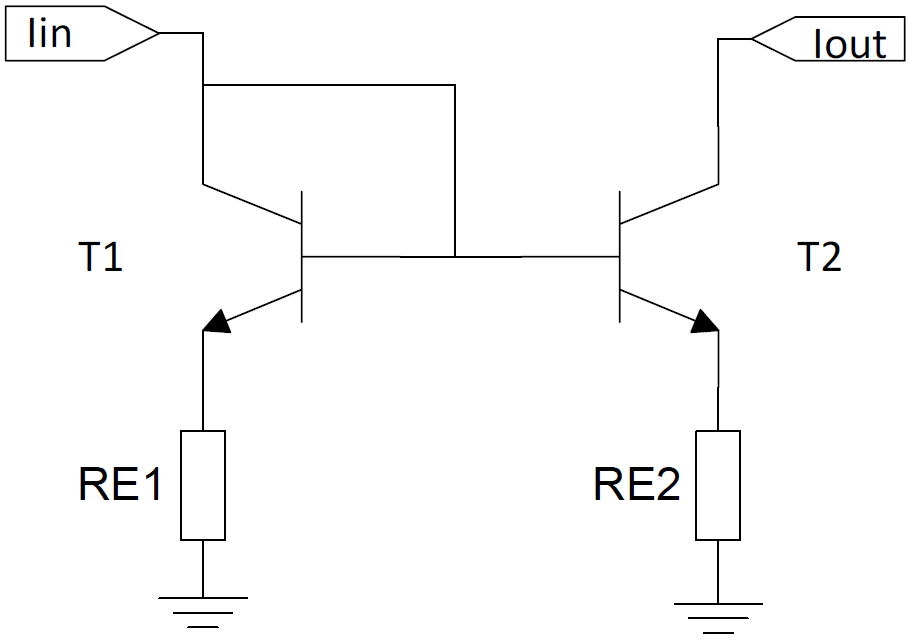
\includegraphics[width=\columnwidth]{images/widlar_stromspiegel.png}
\end{minipage}
\hfill
\begin{minipage}[c]{0.63\columnwidth}
    $$ \boxed{I_{\rm out} = I_{\rm in} \frac{R_{\rm E1}}{R_{\rm E2}} } $$
\end{minipage}


\subsubsection{Stromspiegel mit Kaskode}

\begin{minipage}[c]{0.28\columnwidth}
    \begin{center}
        \myul{\textbf{Stromspiegel}}

        \vspace{0.1cm}

        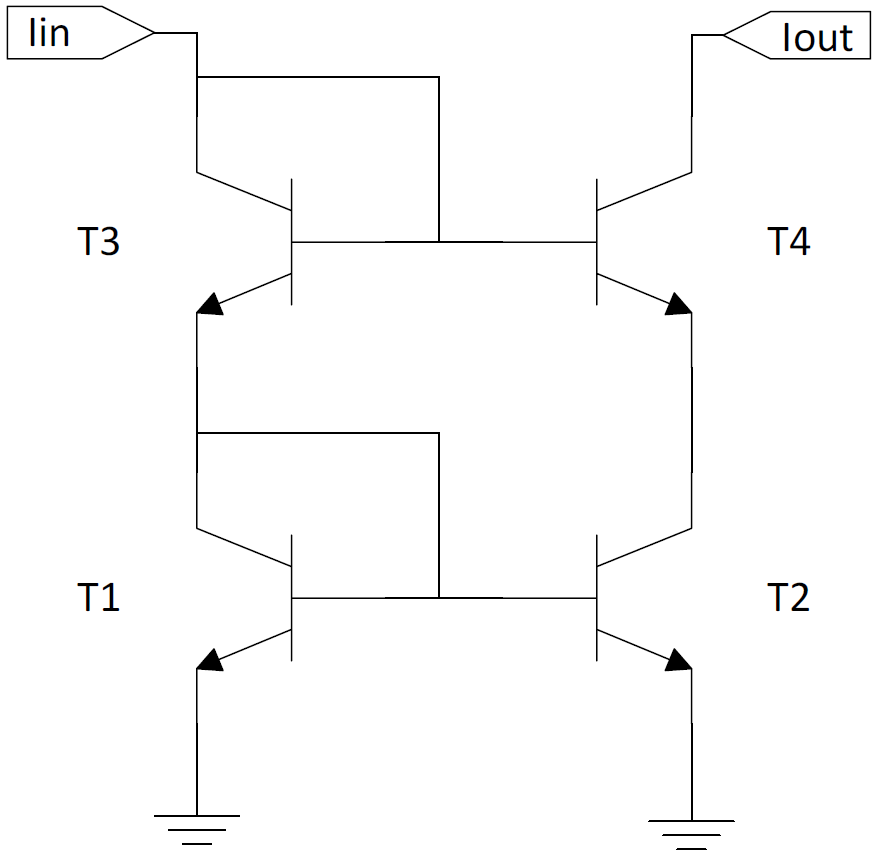
\includegraphics[width=\columnwidth]{images/kaskode.png}
    \end{center}
\end{minipage}
\hfill
\begin{minipage}[c]{0.28\columnwidth}
    \begin{center}
        \myul{\textbf{Funktionsweise}}

        \vspace{0.1cm}

        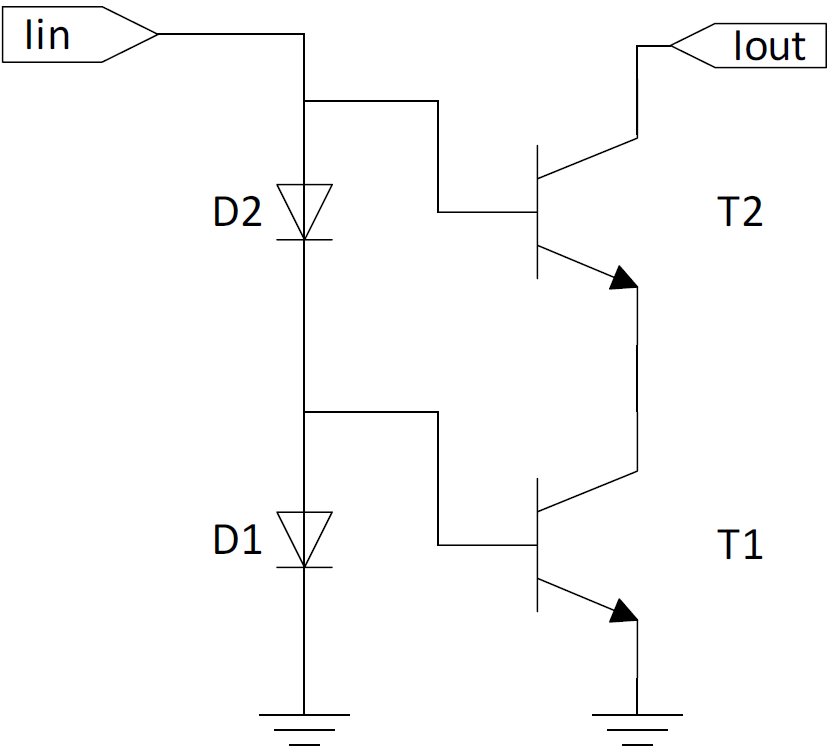
\includegraphics[width=\columnwidth]{images/kaskode_funktionsweise.png}
    \end{center}
\end{minipage}
\hfill
\begin{minipage}[c]{0.4\columnwidth}
    \begin{tabular}{ll@{}}
        $I_{\rm out}$   & Entspricht Kollektorstrom                        \\
                        & von $T_4$                                         \\
        $T_1$           & Als Diode beschaltet                              \\ 
                        & \textrightarrow\ $V_{\rm BE,1} = V_{\rm BE,2}$    \\
                        & \textrightarrow\ $IC_{\rm T1} = IC_{\rm T2}$      \\
        $T_3$           & Als Diode beschaltet                              \\
                        & \textrightarrow\ $V_{\rm CE,2} = 0.7 \, \volt$    \\
        $T_4$           & In Basisschaltung 
        \end{tabular}
\end{minipage}


\subsection{Differenzverstärker}

Differenzverstärker werden als Eingangsstufen von OpAmps oder Highest Speed Logik (LVDS, CML, ECL) eingesetzt. 


\subsubsection{Transistorpaar mit Emitterspannungen $\bm{V_E = 0 \, \volt}$}

\begin{minipage}[c]{0.35\columnwidth}
    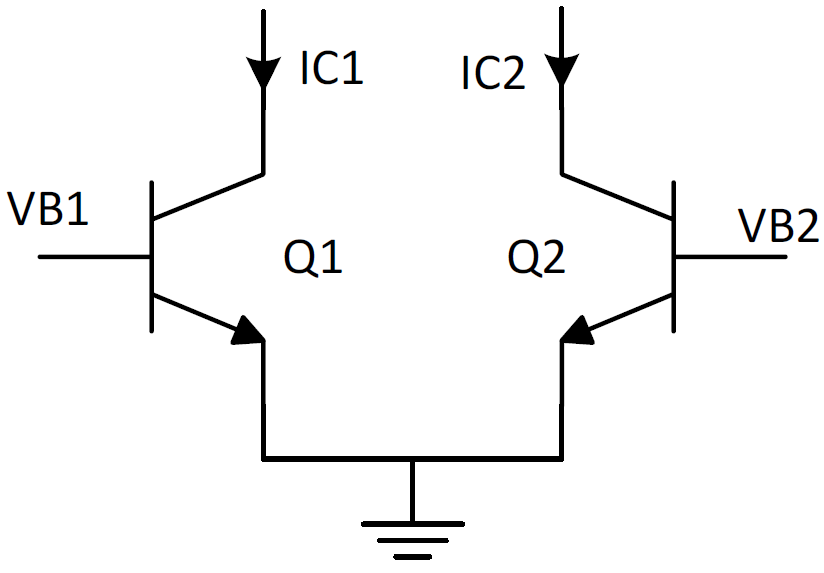
\includegraphics[width=\columnwidth]{images/transistorpaar.png}
\end{minipage}
\hfill
\begin{minipage}[c]{0.6\columnwidth}
    \raggedright
    Kleines $\Delta V$ führt zu grossem $\Delta I$
    
    \vspace{0.2cm}

    \begin{itemize}
        \item $V_{\rm B1} = V_{\rm BE0} + V_D = 0.7 \, \volt + V_D$
        \item $V_{\rm B2} = V_{\rm BE0}$ 
    \end{itemize}

    $$ \boxed{ \frac{I_{\rm C1}}{I_{\rm C2}} =  \frac{I_C ( V_{\rm BE0} + V_D)}{I_C (V_{\rm BE0} ) } = e^{\frac{V_D}{n \cdot V_T}} } $$
\end{minipage}


\subsubsection{Differenzstufe mit Stromquelle $\bm{I_{\rm BIAS}}$}

\begin{minipage}[c]{0.35\columnwidth}
    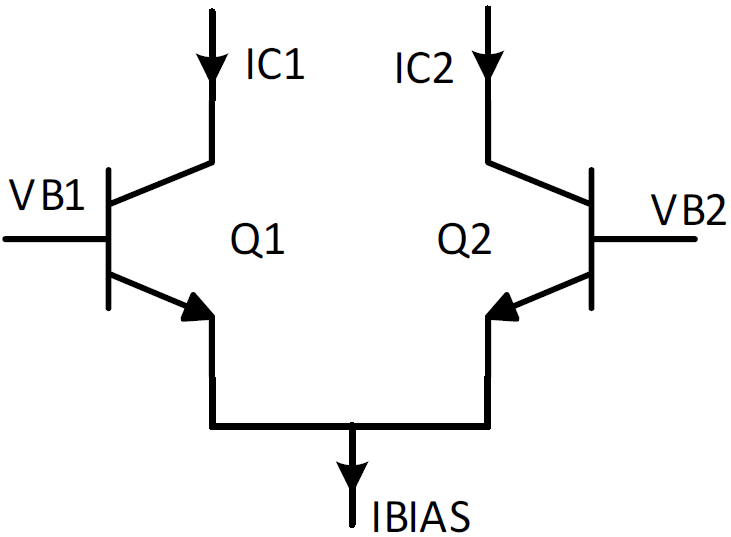
\includegraphics[width=\columnwidth]{images/differenzstufe_IBIAS.png}
\end{minipage}
\hfill
\begin{minipage}[c]{0.6\columnwidth}
    \raggedright

    \begin{itemize}
        \item $I_{\rm BIAS} = I_{\rm C1} + I_{\rm C2} = \const$
        \item $V_{\rm BE2} = V_{\rm B2} - V_E$
        \item $V_{\rm BE1} = V_{\rm BE2} + V_D$
    \end{itemize}

    $$ \boxed{ I_{\rm C1} = \beta \cdot I_S \cdot e^{\frac{V_{\rm BE2} + V_D}{n \cdot V_T}} = I_{\rm C2} \cdot e^{\frac{V_D}{n \cdot V_T}} } $$
    $$ \boxed{ I_{\rm BIAS} \approx I_{\rm C1} + I_{\rm C2} = I_{\rm C2} \cdot ( e^{\frac{V_D}{n \cdot V_T}} + 1) } $$
\end{minipage}


\subsubsection{Differenzstufe mit Stromquelle \& Kollektorwiderstand}

\begin{minipage}[c]{0.4\columnwidth}
    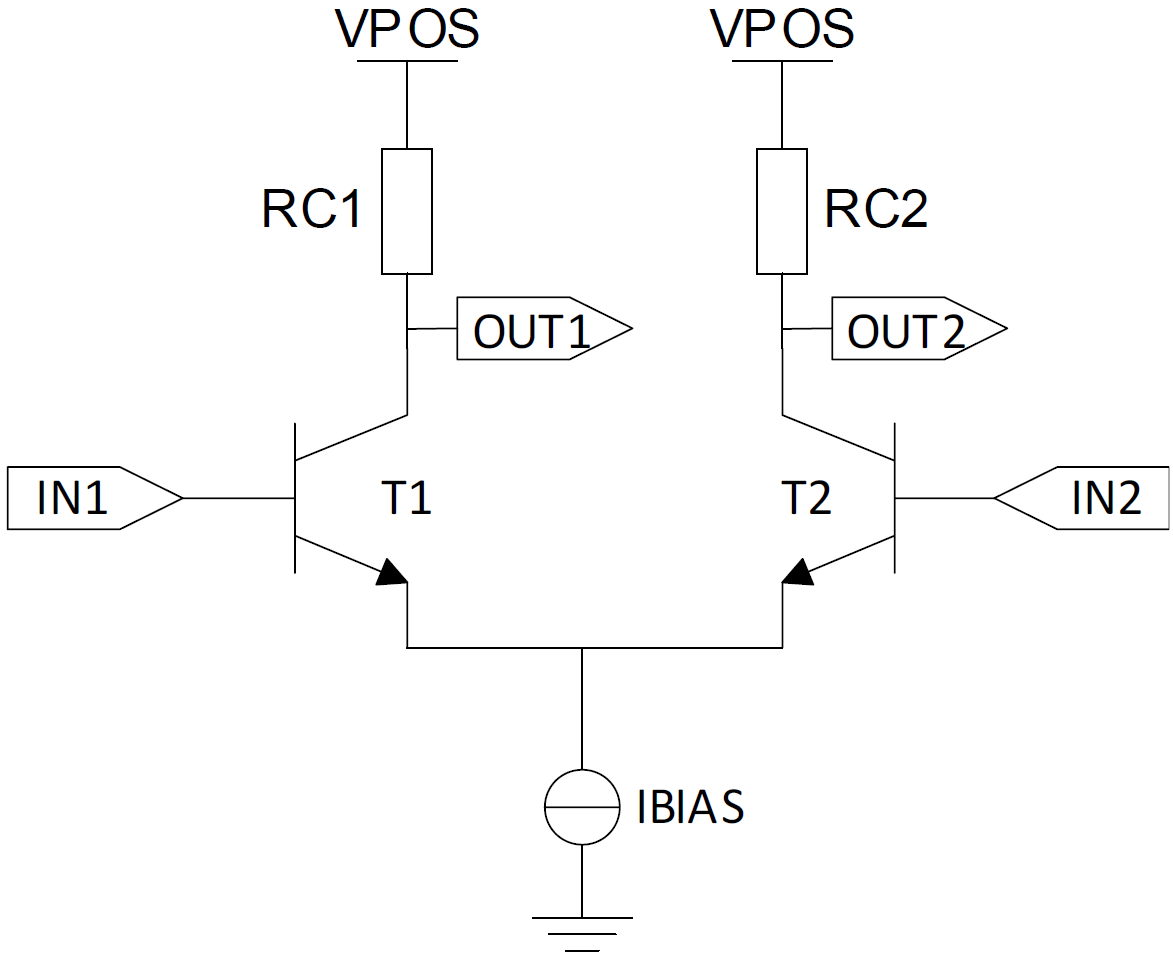
\includegraphics[width=\columnwidth]{images/differenzstufe_kollektorwiderstand.png}
\end{minipage}
\hfill
\begin{minipage}[c]{0.55\columnwidth}
    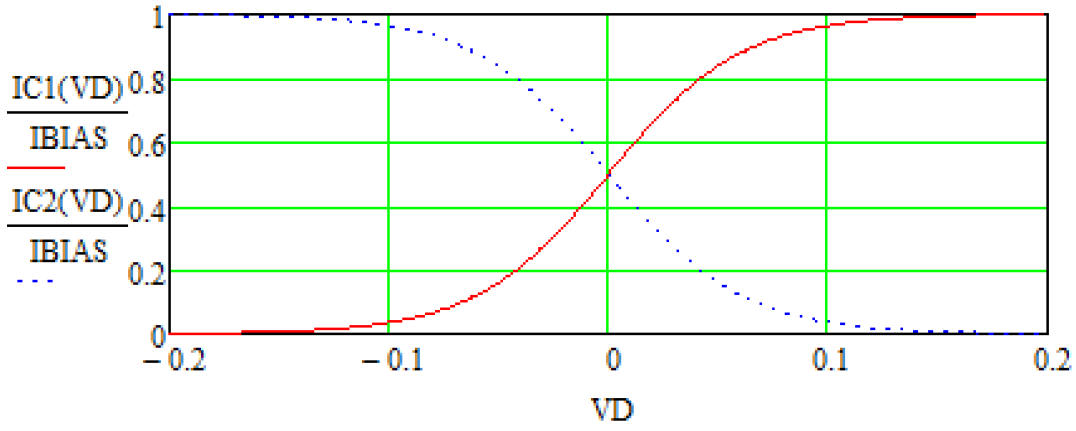
\includegraphics[width=\columnwidth]{images/differenzstufe_kollektorwiderstand_strom.png}
\end{minipage}

\vspace{0.2cm}

\begin{itemize}
    \item $V_D = 0$ durch beide Transistoren fliesst $\frac{I_{\rm BIAS}}{2}$
    \item $|V_D| = 200 \, \milli \volt$ ganzer Strom durch einen Transistor
    \item Im Bereich $\pm 100 \, \milli \volt$ teilt sich Strom auf
    \item $|V_D| < 200 \, \milli \volt$ $V_{\rm out} = V_{\rm out,0} + A \cdot \Delta V_{\rm in}$ \\
        $V_{\rm out,0}$ entspricht Ausgangsspannung @ $V_{\rm in1} = V_{\rm in2} $
\end{itemize}

\columnbreak


		\section{Transistorverstärker}

\subsection{Differenzstufen (Erweiterung)}

\subsubsection{Differenzstufe mit $\bm{I_{\rm BIAS}}$}

\begin{tabular}{ll}
    Differenz Eingangsspannungen:   & $V_D = V_{\rm B1} - V_{\rm B2}$       \\
    Differnz Ströme:                & $\diff I_C = I_{\rm C1} - I_{\rm C2}$
\end{tabular}

\vspace{0.2cm}
\textbf{Arbeitspunkt} für Differenzstufen meistens bei $V_{\rm B1} = V_{\rm B2}$

\vspace{0.2cm}

\begin{minipage}[c]{0.3\columnwidth}
    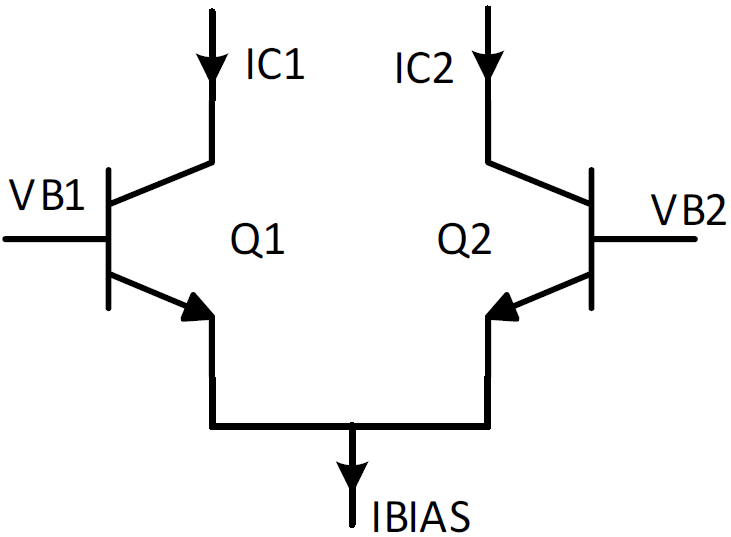
\includegraphics[width=\columnwidth]{images/differenzstufe_IBIAS.png}
\end{minipage}
\hfill
\begin{minipage}[c]{0.68\columnwidth}
    $$ \boxed{ \diff I_C(V_D) = I_{\rm BIAS} \cdot \tanh \Bigg( \frac{V_D}{2 \cdot n \cdot V_T} \Bigg) } $$
    $$ \boxed{ \frac{\diff I}{\diff V_{\rm in}} = I_{\rm BIAS} \cdot \frac{1 - \tanh \Big( \frac{V_D}{2 \cdot n \cdot V_T} \Big)^2 }{2 \cdot n \cdot V_T} } $$
\end{minipage}

\vspace{0.2cm}

$$ \boxed{ gm =  \frac{\diff I_C(V_D)}{\diff V_D} = \frac{I_{\rm BIAS}}{2 \cdot n \cdot V_T}  \cdot \Bigg( 1 - \tanh \Big( \frac{V_D}{2 \cdot n \cdot V_T} \Big)^2 \Bigg) } $$
$$ \boxed{ \text{Für } V_D = 0: \;  gm_{\rm DiffStufe} = \frac{I_{\rm BIAS}}{2 \cdot n \cdot V_T} } $$


\subsubsection{Differenzverstärker}

\begin{minipage}[c]{0.48\columnwidth}
    $$ \Delta V_{\rm in} = V_{\rm in1} - V_{\rm in2} $$
\end{minipage}
\hfill
\begin{minipage}[c]{0.48\columnwidth}
    $$ \Delta V_{\rm out} = V_{\rm out1} - V_{\rm out2} $$
\end{minipage}

\vspace{0.2cm}

\begin{minipage}[c]{0.35\columnwidth}
    \begin{center}
        \myul{\textbf{Schaltung}}

        \vspace{0.2cm}

        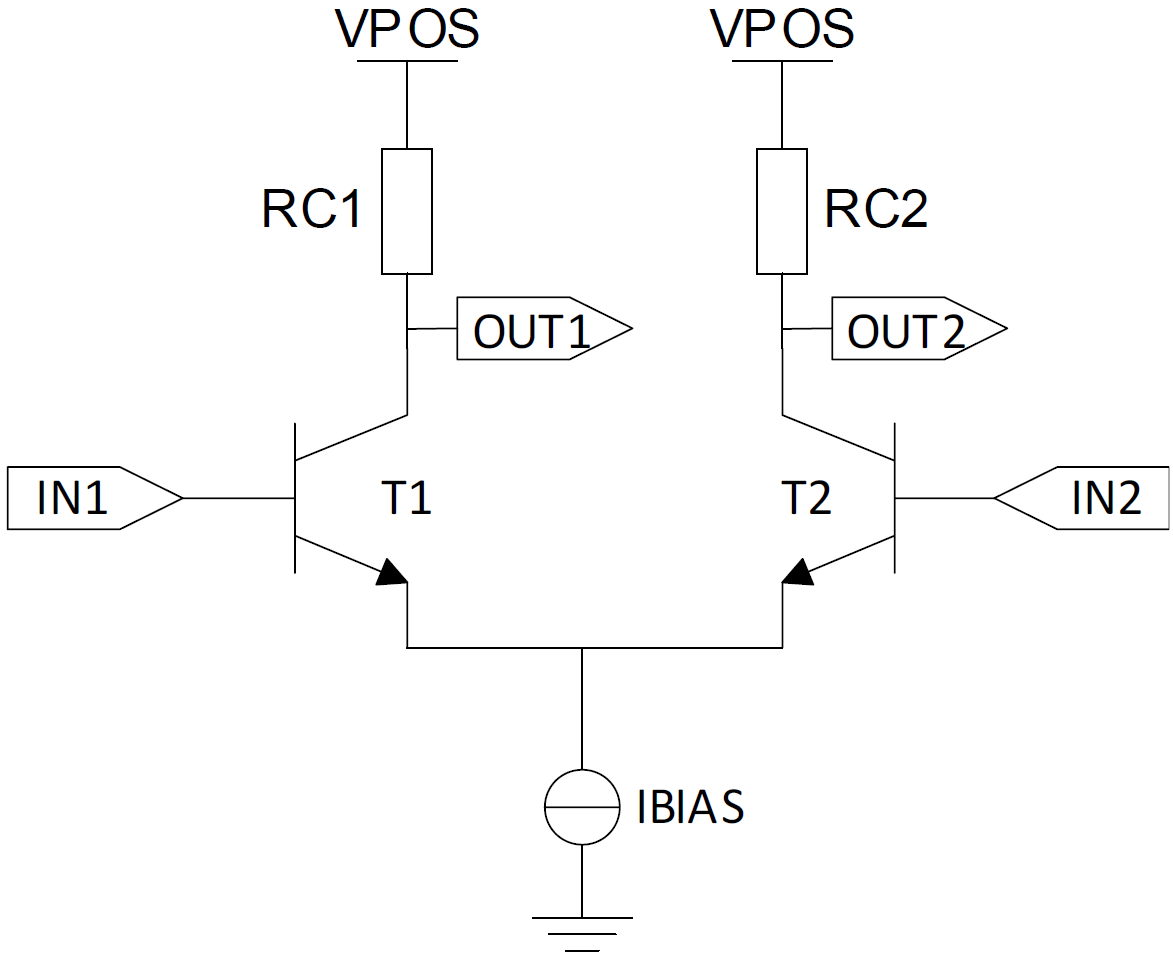
\includegraphics[width=\columnwidth]{images/differenzstufe_kollektorwiderstand.png}
    \end{center}
\end{minipage}
\hfill
\begin{minipage}[c]{0.55\columnwidth}
    \begin{center}
        \myul{\textbf{Kleinsignal-Ersatzschaltung}}

        \vspace{0.2cm}

        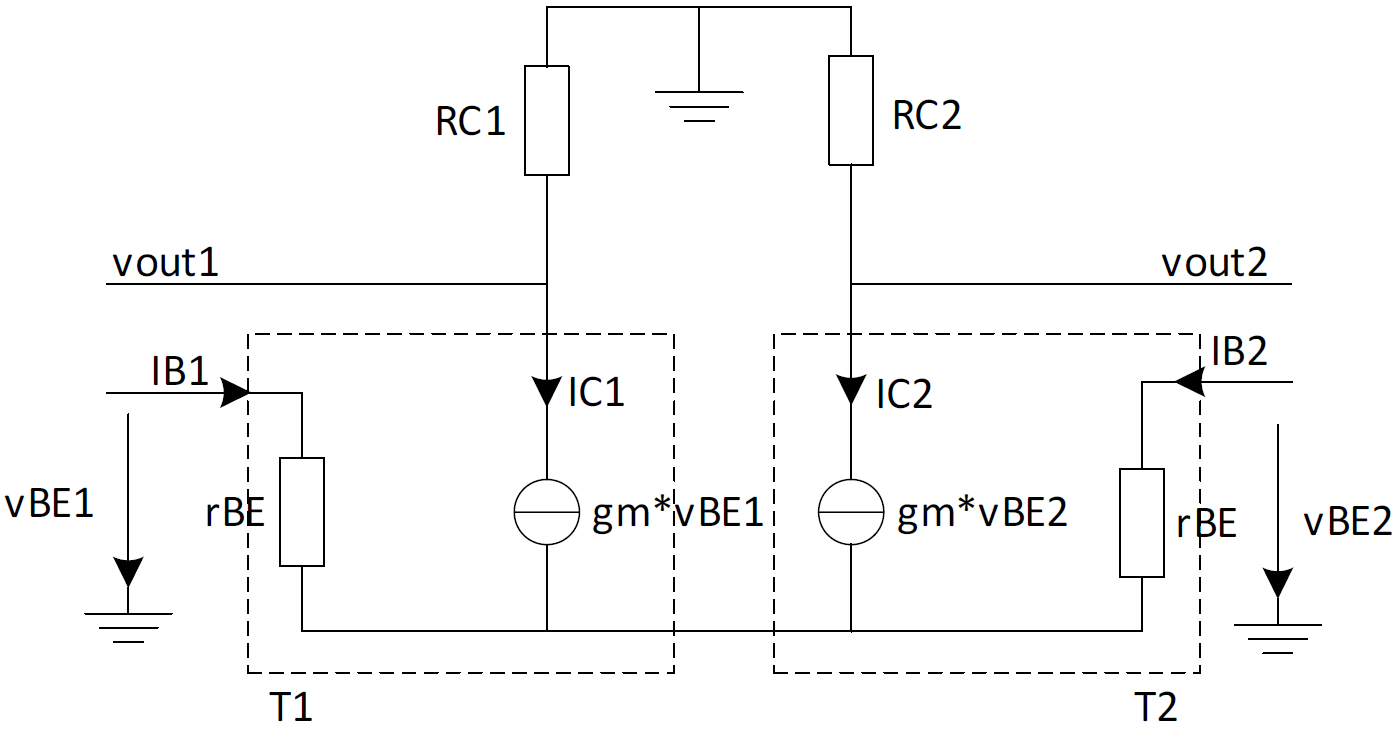
\includegraphics[width=\columnwidth]{images/differenzstufe_kollektorwiderstand_kleinsignalersatzschlatung.png}
    \end{center}
\end{minipage}

\vspace{0.2cm}

\begin{itemize}
    \item Arbeitspunkt bei $ V_{\rm in1} = V_{\rm in2} $
    \item $\frac{I_{\rm BIAS}}{2}$ fliesst durch $T_1$ bzw. $T_2$
    \item Aus Kleinsignalersatzschaltung: $I_{\rm C2} + I_{\rm B2} = - (I_{\rm C1} + I_{\rm B1})$
    \item $v_{\rm BE1} = \frac{\Delta V_{\rm in}}{2}$ und $v_{\rm BE2} = - \frac{\Delta V_{\rm in}}{2}$
\end{itemize}


$$ \boxed{ gm = \frac{\diff I_{\rm C1}}{\diff V_{\rm BE1}} = \frac{I_{\rm C1}}{n \cdot V_T} = \frac{I_{\rm BIAS}}{2 \cdot n \cdot V_T} } \quad \boxed{ r_{\rm BE} = \frac{2 \cdot \beta \cdot n \cdot V_T}{I_{\rm BIAS}} } $$
$$ \boxed{ \Delta V_{\rm out1} = - \frac{1}{2} \Delta V_{\rm in} \cdot gm \cdot R_{\rm C1} } \quad \boxed{ \Delta V_{\rm out2} = \frac{1}{2} \Delta V_{\rm in} \cdot gm \cdot R_{\rm C2} } $$
$$ \boxed{ \text{Verstärkung: } A = \frac{\Delta V_{\rm out}}{\Delta V_{\rm in}} = - gm \cdot R_C = - \frac{I_{\rm BIAS}}{2 \cdot n \cdot V_T} \, R_C } $$ 


\subsubsection{Differenzstufe mit Emitterfolger}

\begin{minipage}[c]{0.35\columnwidth}
    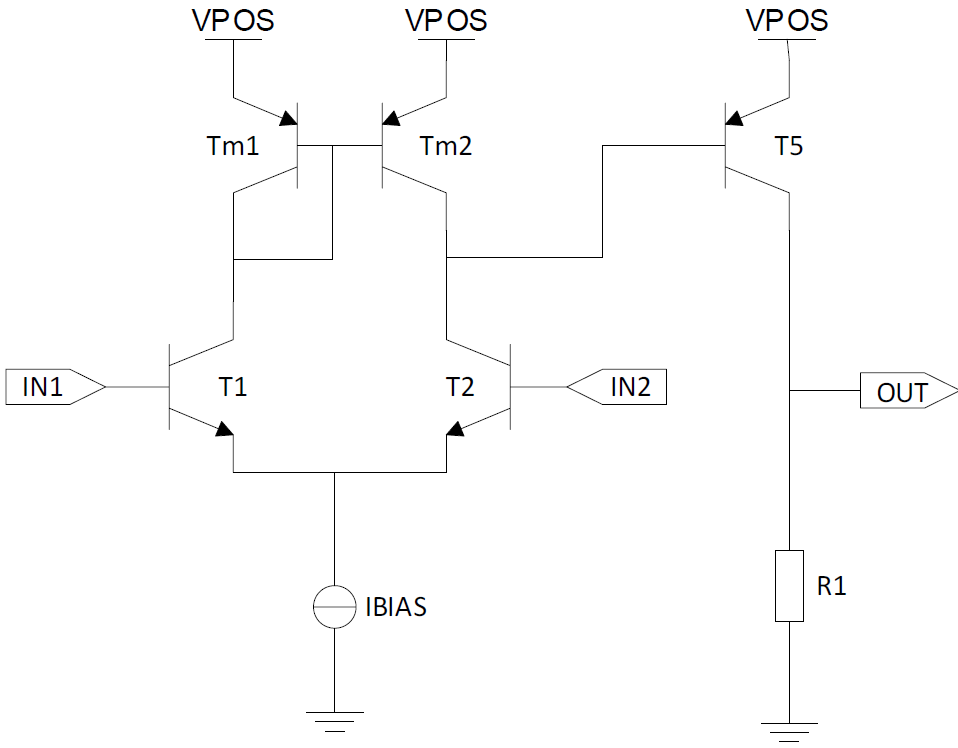
\includegraphics[width=\columnwidth]{images/differenzstufe_emitterfolger.png}
\end{minipage}
\hfill
\begin{minipage}[c]{0.55\columnwidth}
    \raggedright

    \begin{itemize}
        \item $I_{\rm out}$ von Diff-Stufe wird von $T_5$ mit Faktor $\beta$ verstärkt
        \item $R_1$ wandelt Strom in Spannung
    \end{itemize}

    \vspace{0.2cm}

    $$ \boxed{ A = \frac{\Delta V_{\rm out}}{\Delta V_{\rm in}} = \beta \cdot R_1 \cdot \frac{I_{\rm BIAS}}{2 \cdot n \cdot V_T} } $$
\end{minipage}


\subsubsection{Differenzverstärker mit Stromspiegel-Last (OTA)}

\begin{minipage}[c]{0.35\columnwidth}
    \begin{center}
        \myul{\textbf{Schaltung}}

        \vspace{0.2cm}

        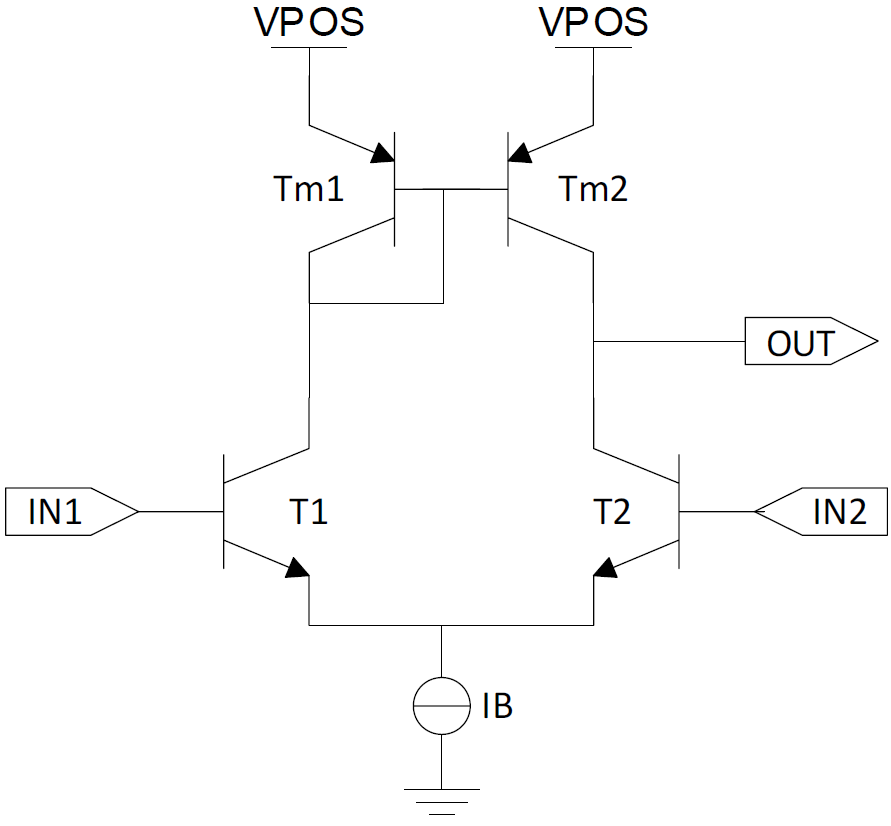
\includegraphics[width=\columnwidth]{images/differenzverstaerker_stromspiegel.png} 
    \end{center}
\end{minipage}
\hfill
\begin{minipage}[c]{0.55\columnwidth}
    \begin{center}
        \myul{\textbf{Kleinsignal-Ersatzschaltung}}

        \vspace{0.2cm}

        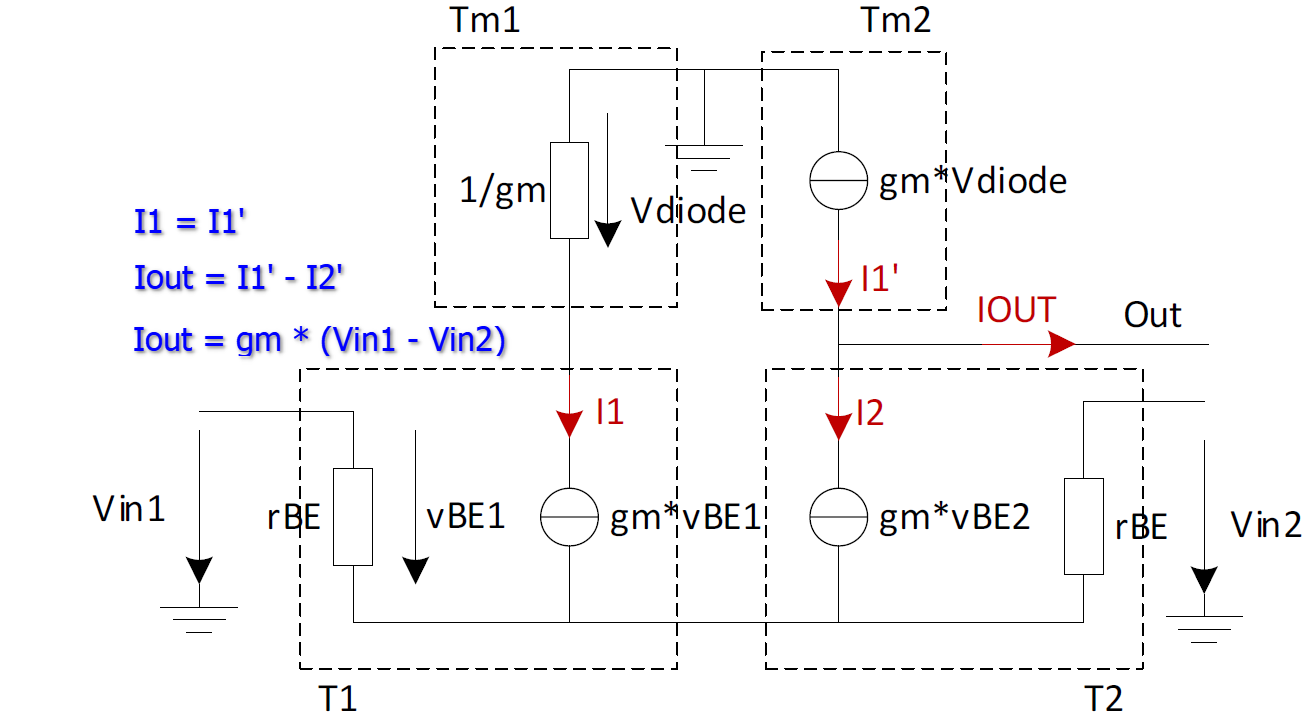
\includegraphics[width=\columnwidth]{images/differnzverstaerker_stromspiegel_ersatzschaltung.png} 
    \end{center}
\end{minipage}

\vspace{0.2cm}

\begin{itemize}
    \item Hoher Ausgangswiderstand $r_{\rm out} = r_{\rm CE1} || r_{\rm CE2}$
    \item Minimale Eingangsspannung: $\approx 0.9 \, \volt$
    \item Maximale Eingangsspannung: $V_{\rm POS} - V_{\rm CE,sat}$
\end{itemize}

$$ \boxed{ gm = \frac{I_{\rm BIAS}}{2 \cdot n \cdot V_T} } \quad \boxed{ I_{\rm out} = gm \cdot (V_{\rm in1} - V_{\rm in2}) = \frac{I_{\rm BIAS}}{2 \cdot n \cdot V_T} \cdot \Delta V_{\rm in} } $$ 


\subsubsection{Differenzstrufe mit Stromquelle}

\begin{minipage}[c]{0.4\columnwidth}
    \begin{center}
        \myul{\textbf{Hochohmige Lasten}}

        \vspace{0.2cm}

        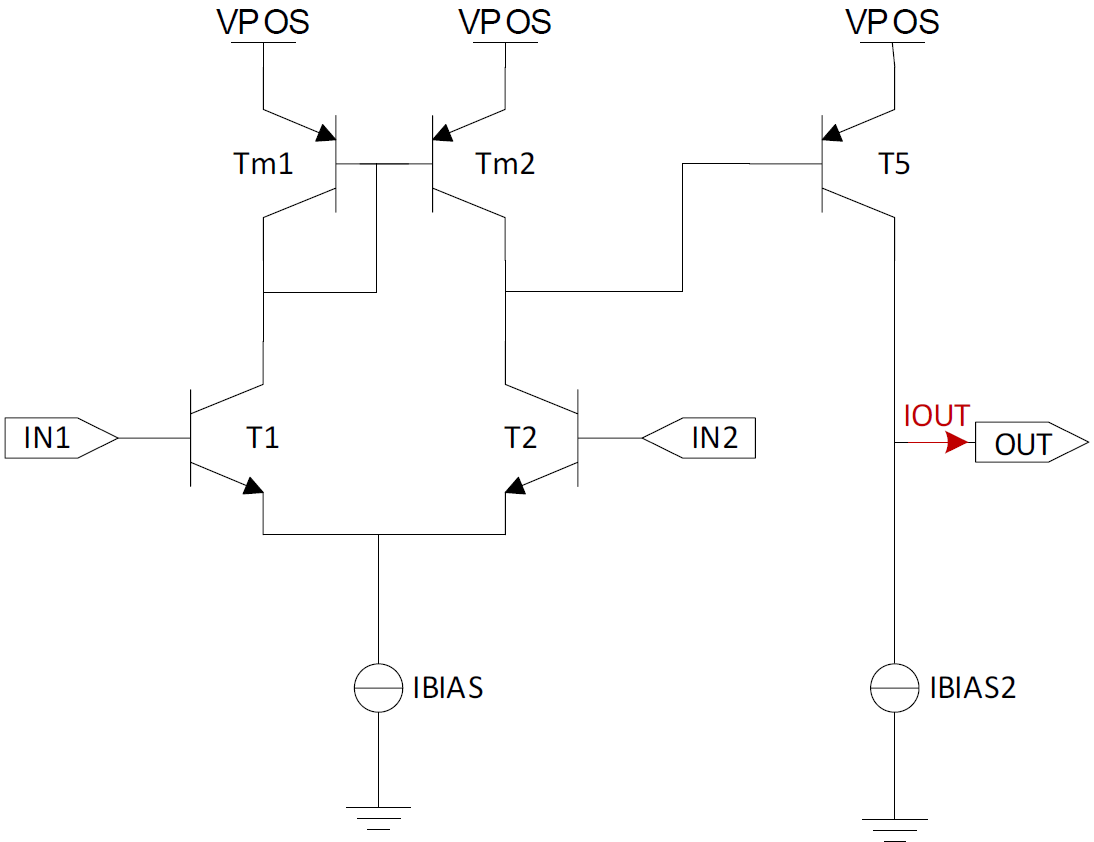
\includegraphics[width=\columnwidth]{images/differenzstufe_stomquelle_hochohmig.png}

        $$ \boxed{ I_{\rm out} = \beta \cdot \frac{I_{\rm BIAS}}{2 \cdot n \cdot V_T} \cdot \Delta V_{\rm in} } $$
    \end{center}    
\end{minipage}
\hfill
\begin{minipage}[c]{0.4\columnwidth}
    \begin{center}
        \myul{\textbf{Niederohmige Lasten}}

        \vspace{0.2cm}

        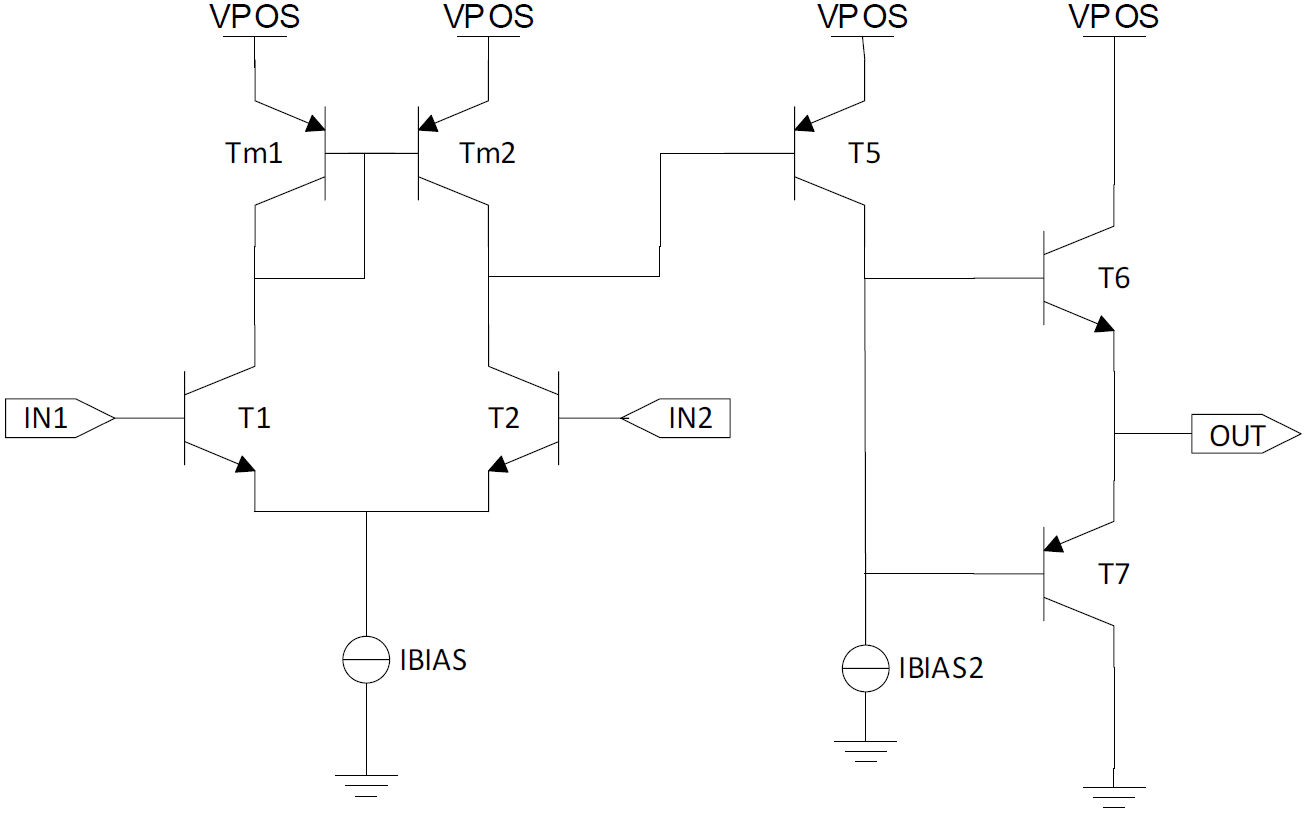
\includegraphics[width=\columnwidth]{images/differenzstufe_stomquelle_niederohmig.png}

        \vspace{0.2cm}

        OTA ergänzt mit Class-B Buffer
    \end{center}
\end{minipage}


\subsubsection{Differenzstufe mit Emitterfolger und Class-AB Buffer}

\begin{minipage}[c]{0.43\columnwidth}
    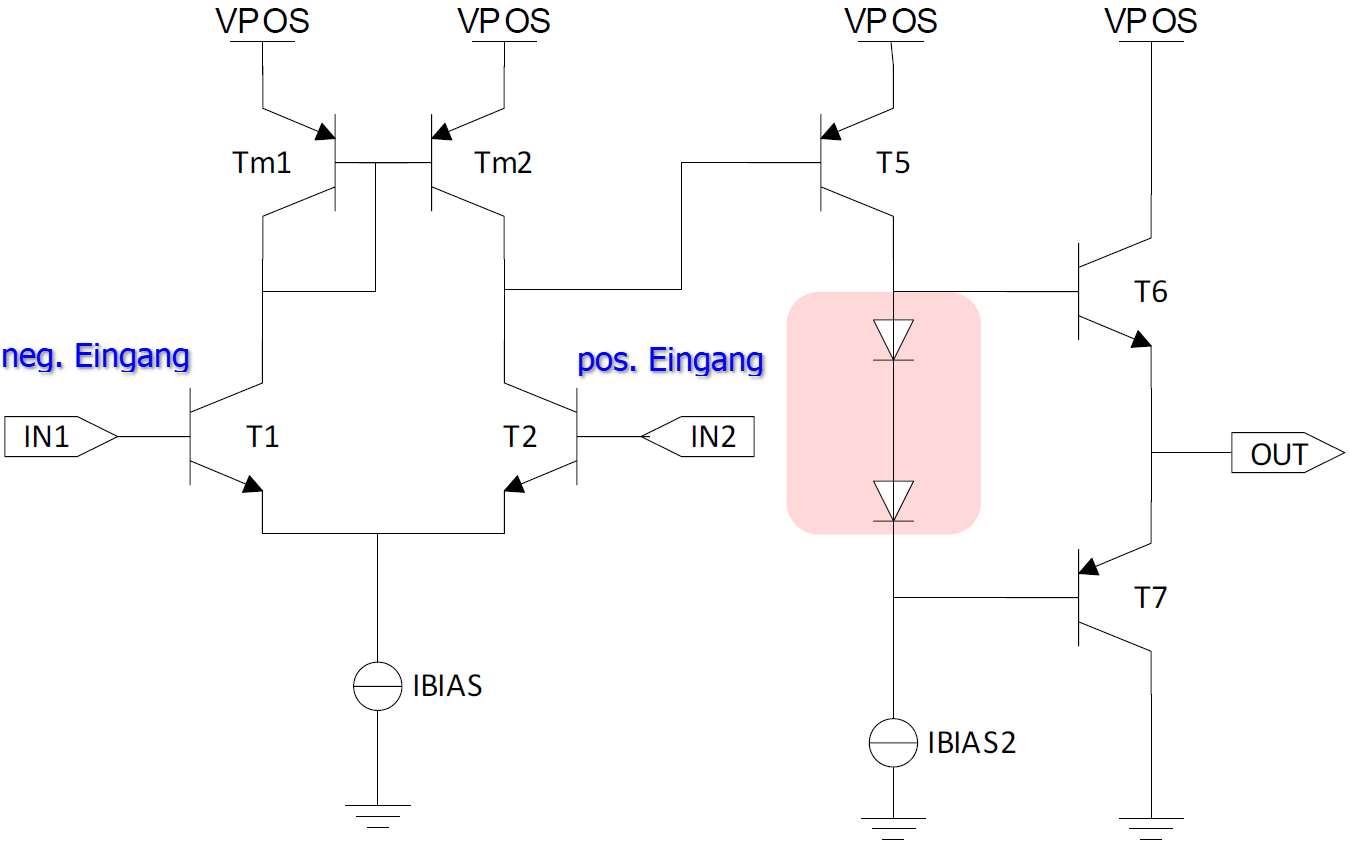
\includegraphics[width=\columnwidth]{images/differenzstufe_emitterfolger_buffer.png} 
\end{minipage}
\hfill
\begin{minipage}[c]{0.53\columnwidth}
    \raggedright

    \begin{itemize}
        \item Erlaubt Verstärkungen $\geq 10'000$
        \item \textbf{Schaltung ist 'Komparator'oder Verstärker mit Rückkopplung auf neg. Eingang}
    \end{itemize}
\end{minipage}


\subsection{Darlington-Schaltung}

Darlington-Schaltungen werden eingesetzt, um grössere Stromverstärkungen zu erzielen.


\subsubsection{Darlington}

\begin{minipage}[c]{0.16\columnwidth}
    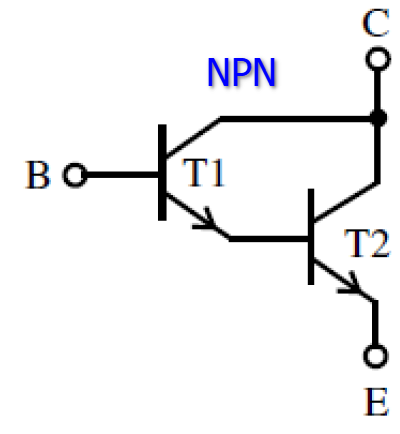
\includegraphics[width=\columnwidth]{images/darlington_npn.png} 
\end{minipage}
\hfill
\begin{minipage}[c]{0.16\columnwidth}
    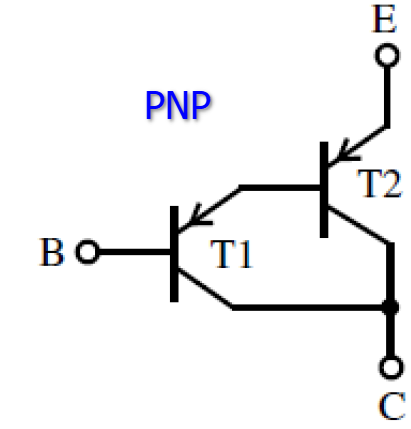
\includegraphics[width=\columnwidth]{images/darlington_pnp.png} 
\end{minipage}
\hfill
\begin{minipage}[c]{0.58\columnwidth}
    $$ \boxed{ V_{\rm BE} = V_{\rm BE1} + V_{\rm BE2} } $$
    $$ \boxed{ \beta = \beta_1 + \beta_2 } $$
\end{minipage}


\subsubsection{Komplementär-Darlington}

\begin{minipage}[c]{0.22\columnwidth}
    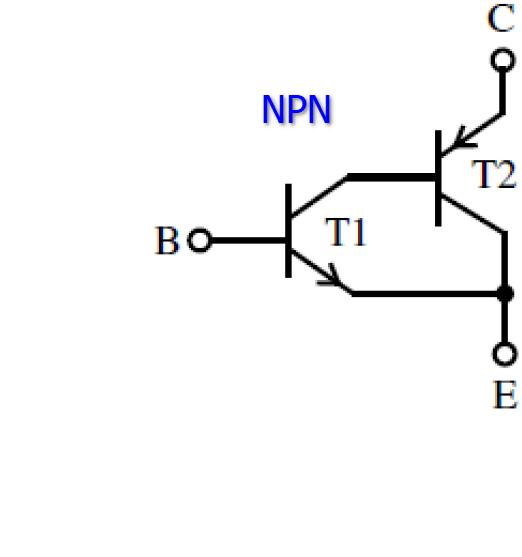
\includegraphics[width=\columnwidth]{images/komplementaer_darington_npn.png} 
\end{minipage}
\hfill
\begin{minipage}[c]{0.22\columnwidth}
    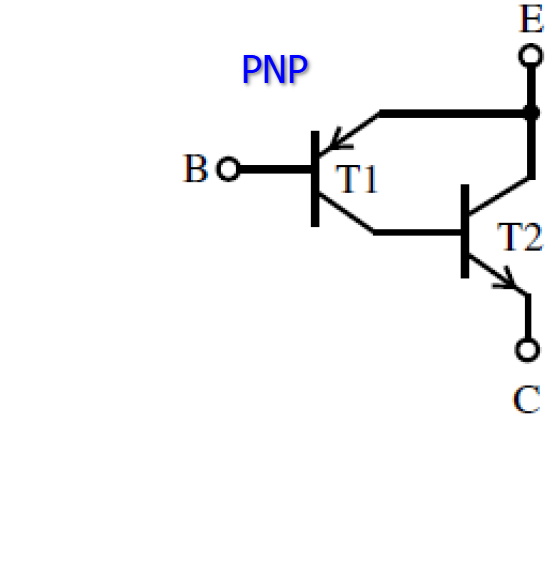
\includegraphics[width=\columnwidth]{images/komplementaer_darington_pnp.png} 
\end{minipage}
\hfill
\begin{minipage}[c]{0.48\columnwidth}
    $$ \boxed{ V_{\rm BE} = V_{\rm BE1} } $$
    $$ \boxed{ \beta = \beta_1 + \beta_2 } $$
\end{minipage}

\vspace{-0.4cm}


\subsection{Verstärker mit Current Feedback OpAmp}

\begin{minipage}[c]{0.32\columnwidth}
    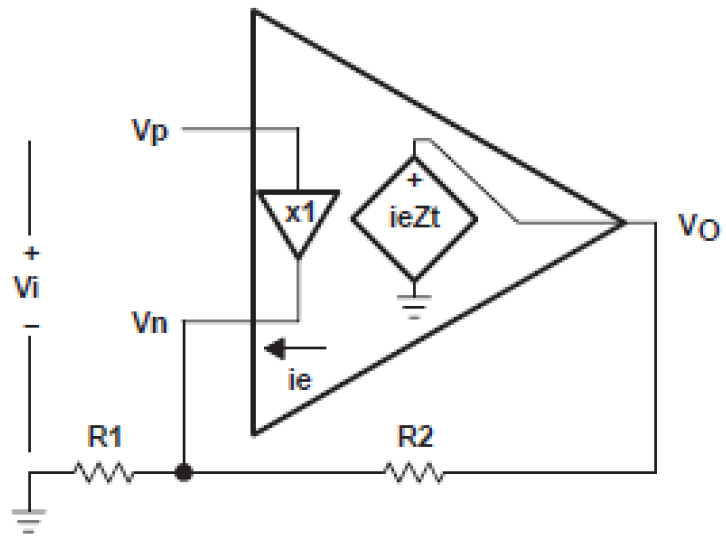
\includegraphics[width=\columnwidth]{images/verstaerker_current_feedback_opv.png} 
\end{minipage}
\hfill
\begin{minipage}[c]{0.63\columnwidth}
    \raggedright

    \begin{itemize}
        \item $Z_t = $ sehr grosse interne Impedanz
        \item $I_e$ regelt sich über Feedback auf 0
        \item Verstärkung wie normaler OpAmp aber viel schneller
    \end{itemize}

    $$ \boxed{ V_p = V_n = V_o \frac{R_1}{R_1 + R_2} } \quad \boxed{ V_o = V_p \, \Bigg( 1 + \frac{R_2}{R_1} \Bigg) } $$
\end{minipage}


		\section{Dioden -- Optoelektronik}

\subsection{Energie eines Photons}

\begin{minipage}[c]{0.3\columnwidth}
	$$ \boxed{ \text{E}_{ph} = h\cdot v = \frac{h\cdot c}{\lambda} } $$
    $$ \left[ E_{\rm ph} \right] = \joule $$
    %\[ \boxed{ \text{P} = n\cdot\frac{h\cdot c}{\lambda}\cdot\frac{1}{\rm t}} \]
\end{minipage}
\hfill
\begin{minipage}[c]{0.68\columnwidth}
    \renewcommand{\arraystretch}{1.4}
    \begin{tabular}{ll}
        $h$         & Plancksches Wirkungsquantum: $6.626 \cdot 10^{-34} \, \joule \, \second$      \\
        $v$         & Frequenz in $\frac{\meter}{\second}$                                          \\
        $c$         & Lichtgeschwindigkeit: $299'792 \, \frac{\kilo \meter}{\second}$               \\
        $\lambda$   & Wellenlänge in $\meter$
    \end{tabular}
\end{minipage}


\subsection{Energie in Elektronenvolt}

\vspace{-0.2cm}

\begin{minipage}[c]{0.3\columnwidth}
    $$ \boxed{ E_{\rm ph \, eV} = h \cdot v = \frac{h \cdot c}{\lambda \cdot q} } $$
\end{minipage}
\hfill
\begin{minipage}[c]{0.68\columnwidth}
    \begin{tabular}{ll}
       $q$  &   Elementarladung eines Elektrons: $1.602 \cdot 10^{-19} \, \ampere \, \second$
    \end{tabular}
\end{minipage}

\medskip

Die Bandlücke $W_g$ von Silizium beträgt $\bm{1.1 \, \mathrm{eV}}$ \textrightarrow\ Wellenlänge von etwa $1.1 \, \micro \meter$
    \end{layout}
\end{document}

